\documentclass[acronym,symbols,table]{fei}

%\usepackage{glossaries}
\usepackage[utf8]{inputenc}
\usepackage{subcaption} 
\renewcommand{\thesubfigure}{\Alph{subfigure}}
\usepackage{graphicx}
\usepackage{amsmath} % for the equation* environment
\usepackage{float}
\usepackage[portuguese]{algorithm2e}
\usepackage{biblatex}
\usepackage{listings}
\usepackage{chngcntr} 
\usepackage{appendix}
\usepackage{gensymb}
\counterwithout{footnote}{chapter}
\usepackage{siunitx}
\sisetup{output-exponent-marker=\ensuremath{\mathrm{e}}}
\renewcommand{\cftfigurepresnum}{Figura }
\setlength{\cftfigurenumwidth}{5.7em}
\usepackage{titling}
\usepackage{comment}

\title{Avaliação do condicionamento do ar da frota L do Metrô de São Paulo}
\author{Ana Sung Marques \\Felipe Estevão Coquito de Mello\\  Gabriel de Souza Simonetti  \\ Gabriel Mola da Silva \\ Netuno Trindade Torrente Rovaroto \\ Victor Salzo Lopes  \\ Vitoria Fedatto Stefaneli}
\cidade{São Bernardo do Campo}
\instituicao{Centro Universitário FEI}

\addbibresource{Referencias.bib}
%\bibliographystyle{plain}
\bibliography{Referencias}
\graphicspath{ {Imagens/}, {Tabelas/}}

%\makeglossaries
%%\newacronym[] {achpt} {ACT} {Aparecido ChupeTão}

\newacronym[longplural=Associações Brasileiras de Normas Técnicas]{abnt}{ABNT}{Associação Brasileira de Normas Técnicas}

\newacronym{ibge}{IBGE}{Instituto Brasileiro de Geografia e Estatística}

\newacronym{ashrae}{ASHRAE}{\textit{American Society of Heating, Refrigerating and Air-Conditioning Engineers}}

\newacronym{nbr}{NBR}{Norma Brasileira}

\newacronym{pmv}{PMV}{\textit{Predicted Mean Vote}}
	
\newacronym{ppd}{PPD}{\textit{Predicted Percentage of Dissatisfied}}
		
\newacronym{vgd}{VGD}{Ventilação Geral Diluidor}
		
\newacronym{vgl}{VGL}{Ventilação Local Exaustora}
		
\newacronym{cfd}{CFD}{\textit{Computational Fluid Dynamics}}
		
\newacronym{pcb}{PCB}{\textit{Printed Circuit Board}}
		
\newacronym{sms}{SMS}{\textit{Short Message Service}}
		
%\newglossaryentry{pi}{parent=greek,type=symbols,name={\ensuremath{\pi}},sort=p,description={número irracional que representa [razão entre a circunferência de qualquer círculo e seu diâmetro]}}
		


\begin{document}

\maketitle

\begin{folhaderosto}
	Trabalho de Conclusão de Curso apresentado ao Centro Universitário FEI, como parte dos requisitos necessários para obtenção do título de Bacharel em Engenharia Mecânica. Orientado pelo Prof. Dr. Cyro Albuquerque Neto.
\end{folhaderosto}

\begin{agradecimentos}

Gostaríamos de expressar nossa mais profunda gratidão ao Centro Universitário FEI, Fundação Educacional Inaciana Padre Sabóia de Medeiros, por nos proporcionar a oportunidade de realizar este trabalho com todo o suporte necessário. Agradecemos especialmente ao nosso orientador, Prof. Dr. Cyro Albuquerque Neto, por sua orientação e apoio contínuos ao longo de todo o projeto.

Estendemos nossos sinceros agradecimentos aos professores Profa. Dra. Leila Bergamasco, Prof. Dr. Reinaldo Bianchi e Prof. Mestre Rodrigo Bernardello, cujas contribuições foram de extrema importância para o desenvolvimento deste trabalho e sua conclusão.

Agradecemos também aos nossos pais e familiares, cujo apoio constante durante esses cinco anos de formação foi inestimável. Sem o suporte emocional, financeiro e moral de nossos entes queridos, não teríamos conseguido superar os desafios e alcançar nossos objetivos acadêmicos. A paciência, compreensão e encorajamento que nos foram oferecidos ao longo dessa jornada foram fundamentais para o nosso sucesso.

Nosso sincero agradecimento ao Metrô de São Paulo e a todos os seus membros que tornaram este projeto possível, desde a idealização até a execução, em especial aos senhores Charles Iury, Fabio G. Cavalcante, Gleyson Freitas e Marcelo Dias de Campos. 

Por fim, gostaríamos de agradecer aos membros da equipe RoboFEI que forneceram suporte técnico em áreas como programação e eletrônica, sendo eles Alexandre Amaral, Alvaro Desan Neto, Guilherme Luis Pauli, João Victor Aguiar, Mestre Leonardo da Costa.

\end{agradecimentos}

\begin{resumo} %REESCREVER NO FINAL DE TUDO

O Metrô de São Paulo, com mais de 600 milhões de quilômetros percorridos e 33 bilhões de passageiros transportados desde sua inauguração em 1974, enfrenta desafios relacionados ao condicionamento de ar em seus carros. Em 2023, as reclamações sobre ventilação e ar-condicionado, vindas do serviço de \textit{SMS}, somaram mais de 8 mil registros, representando $21\%$ do total. Este trabalho, desenvolvido em parceria com o Metrô de São Paulo e o Centro Universitário FEI, buscou avaliar o conforto térmico dos passageiros e propor melhorias no sistema de condicionamento de ar. O estudo envolveu a instrumentação de um carro com sensores para monitorar temperatura, umidade, concentração de ${CO}_{2}$ e pressão barométrica. Os dados coletados foram analisados com base nas normas técnicas vigentes da ABNT e \textit{ASHRAE}, correlacionando-os às reclamações e dados recebidos. Simulações em elementos finitos no \textit{Software Ansys} permitiram avaliar a eficiência do sistema atual, principalmente a distribuição de ar nos carros. Cálculos de balanço de energia foram realizados, buscando um maior embasamento teórico para determinar o conforto térmico do espaço. Os resultados apontaram que a ocupação do carro não tem grande influência na temperatura interna, além disso, parâmetros como umidade e dióxido de carbono (${CO}_{2}$) ultrapassaram os limites normativos. Observou-se ainda que a ocupação elevada do carro contribui para o aumento na concentração de ${CO}_{2}$. As simulações revelaram falhas na distribuição de ar, especialmente próximas às portas, devido à concentração de passageiros. Diante disso, conclui-se que é essencial revisar o sistema de ventilação, incluindo a instalação de sensores adicionais para monitoramento contínuo de umidade e vazão do ar, permitindo um maior controle destes parâmetros por parte da equipe do Metrô. Ademais, recomenda-se o fortalecimento do sistema de coleta de reclamações, ampliando sua abrangência para alcançar um número maior de usuários e refletir, de forma mais precisa, as percepções e experiências dos passageiros em relação ao conforto térmico.


\palavraschave{Metrô. Condicionamento de ar. Transporte público. Simulação computacional. Sensoriamento.}

\end{resumo}

\begin{abstract} %REESCREVER  NO FINAL DE TUDO

The Metrô de São Paulo, with more than 600 million kilometers traveled and 33 billion passengers transported since its inauguration in 1974, faces challenges related to air conditioning in its cars. In 2023, complaints about ventilation and air conditioning from the \textit{SMS} service amounted to more than 8,000 records, representing $21\%$ of the total. This work, carried out in partnership with Metrô de São Paulo and Centro Universitário FEI, sought to assess the thermal comfort of passengers and propose improvements to the air conditioning system. The study involved instrumentation of a car with sensors to monitor temperature, humidity, ${CO}_{2}$ concentration and barometric pressure. The data collected was analyzed based on current ABNT and \textit{ASHRAE} technical standards, correlating it to the complaints and data received. Finite element simulations in \textit{Ansys software} made it possible to evaluate the efficiency of the current system, especially the distribution of air in the cars. Energy balance calculations were carried out, seeking a greater theoretical basis for determining the thermal comfort of the space. The results showed that car occupancy does not have much influence on the internal temperature, and that parameters such as humidity and carbon dioxide (${CO}_{2}$) exceeded the normative limits. It was also observed that high car occupancy contributes to an increase in the concentration of ${CO}_{2}$. The simulations revealed flaws in air distribution, especially near the doors, due to the concentration of passengers. In view of this, it is concluded that it is essential to revise the ventilation system, including the installation of additional sensors for continuous monitoring of humidity and air flow, allowing greater control of these parameters by the Metrô's staff. Furthermore, it is recommended that the system for collecting complaints be strengthened, expanding its scope to reach a greater number of users and more accurately reflecting passengers perceptions and experiences in relation to thermal comfort.

    \keywords{Metrô. Air conditioning. Public transport. Computer simulation. Sensing.} 

\end{abstract}

\listoffigures
\listoftables
%\printglossaries
%\printglossary[type=\acronymtype]
\tableofcontents

\chapter{Introdução}

A Companhia do Metropolitano de São Paulo – Metrô teve sua primeira atividade no dia 14 de setembro de 1974, e desde então percorreu uma distancia total de mais de 600 milhões de Quilômetros e transportou cerca de 33 Bilhões de passageiros, sendo assim considerada um incrível marco na engenharia e planejamento urbano, segundo \textcite{inicio} e \textcite{g1}.
Ela surgiu como uma solução vital para o transporte das pessoas na região metropolitana de São Paulo, que posteriormente, com o rápido crescimento populacional, se tornou cada vez mais essencial na vida dos paulistas.

No entanto, por mais que o Metrô seja uma excelente proposta para mitigar os problemas de tráfego e transporte enfrentados na metrópole, ele enfrenta diversos desafios, incluindo a lotação em horários de pico, com milhões de pessoas fazendo uso deste meio de transporte todos os dias, além da necessidade de melhoria na manutenção e infraestrutura.

Considerando a enorme quantidade de pessoas utilizando este meio de transporte, uma das maiores adversidades para os responsáveis é fornecer ambientes internos agradáveis e seguros. Isso destaca ainda mais a necessidade de estudar a respeito do conforto térmico e da qualidade do ar dentro dos carros, para avaliar a situação atual e desenvolver e proporcionar uma solução para esta problemática.

\section{Motivação}

A cidade de São Paulo é a maior cidade do Brasil, com mais de 11 milhões de habitantes \cite{IBGE}, e com seu crescimento acelerado se faz necessário abordar discussões a respeito de soluções para a mobilidade urbana na cidade. Portanto, cria-se a necessidade de incentivar a utilização de transportes coletivos. Desse modo, proporcionar uma experiência agradável nos transportes públicos auxilia no desenvolvimento positivo da mobilidade urbana de São Paulo, trazendo mais pessoas para os transportes coletivos.

Segundo o \textcite{cnt} os transportes públicos foram responsáveis por 15,3 milhões de viagens diárias no ano de 2017 na grande São Paulo, o que equivale a um total de $37\%$ do total dos deslocamentos da cidade, visto na Figura \ref{fig:cnt}. Os serviços de trilhos têm aproximadamente 4 milhões de viagens diárias, o que corresponde a $25\%$ entre os transportes públicos. Considerando esse número expressivo o suficiente, os serviços oferecidos pelo Metrô de São Paulo são fundamentais para a vida das pessoas atualmente, logo, é essencial olhar as problemáticas que o mesmo possui.

\begin{figure}[!htb] 
 \centering
    \caption{Distribuição das viagens na grande São Paulo}
    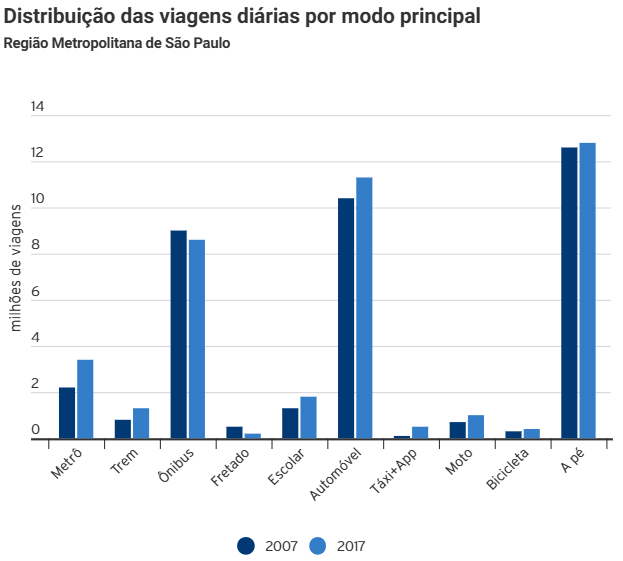
\includegraphics[width=0.8\linewidth]{Imagens/Distruibuicao.png}
    \smallcaption{Fonte: \textcite{cnt}.}
    \label{fig:cnt}
\end{figure}

\newpage 

No portal oficial \textcite{MetroSP} uma das maiores problemáticas atribuídas ao Metrô de São Paulo reside na qualidade do ar e na temperatura interna nos carros, sendo que no ano de 2023, do total de 42.380 reclamações, $21\%$ foram referentes a ar-condicionado. Dentre estas, a principal queixa referente foi ao calor, com mais de 8 mil reclamações, fazendo-se possível observar essas informações nas Figuras \ref{fig:grafico_total} e \ref{fig:grafico_ar}. Logo, com essa questão ressaltada, a urgência de um estudo que proponha a solução para os problemas de ventilação dentro dos carros da frota do Metrô é palpável.

\begin{figure}[!htb]
	\centering
	\begin{minipage}{0.5\textwidth}
		\caption{Reclamações totais do Metrô de São Paulo no ano de 2023}
		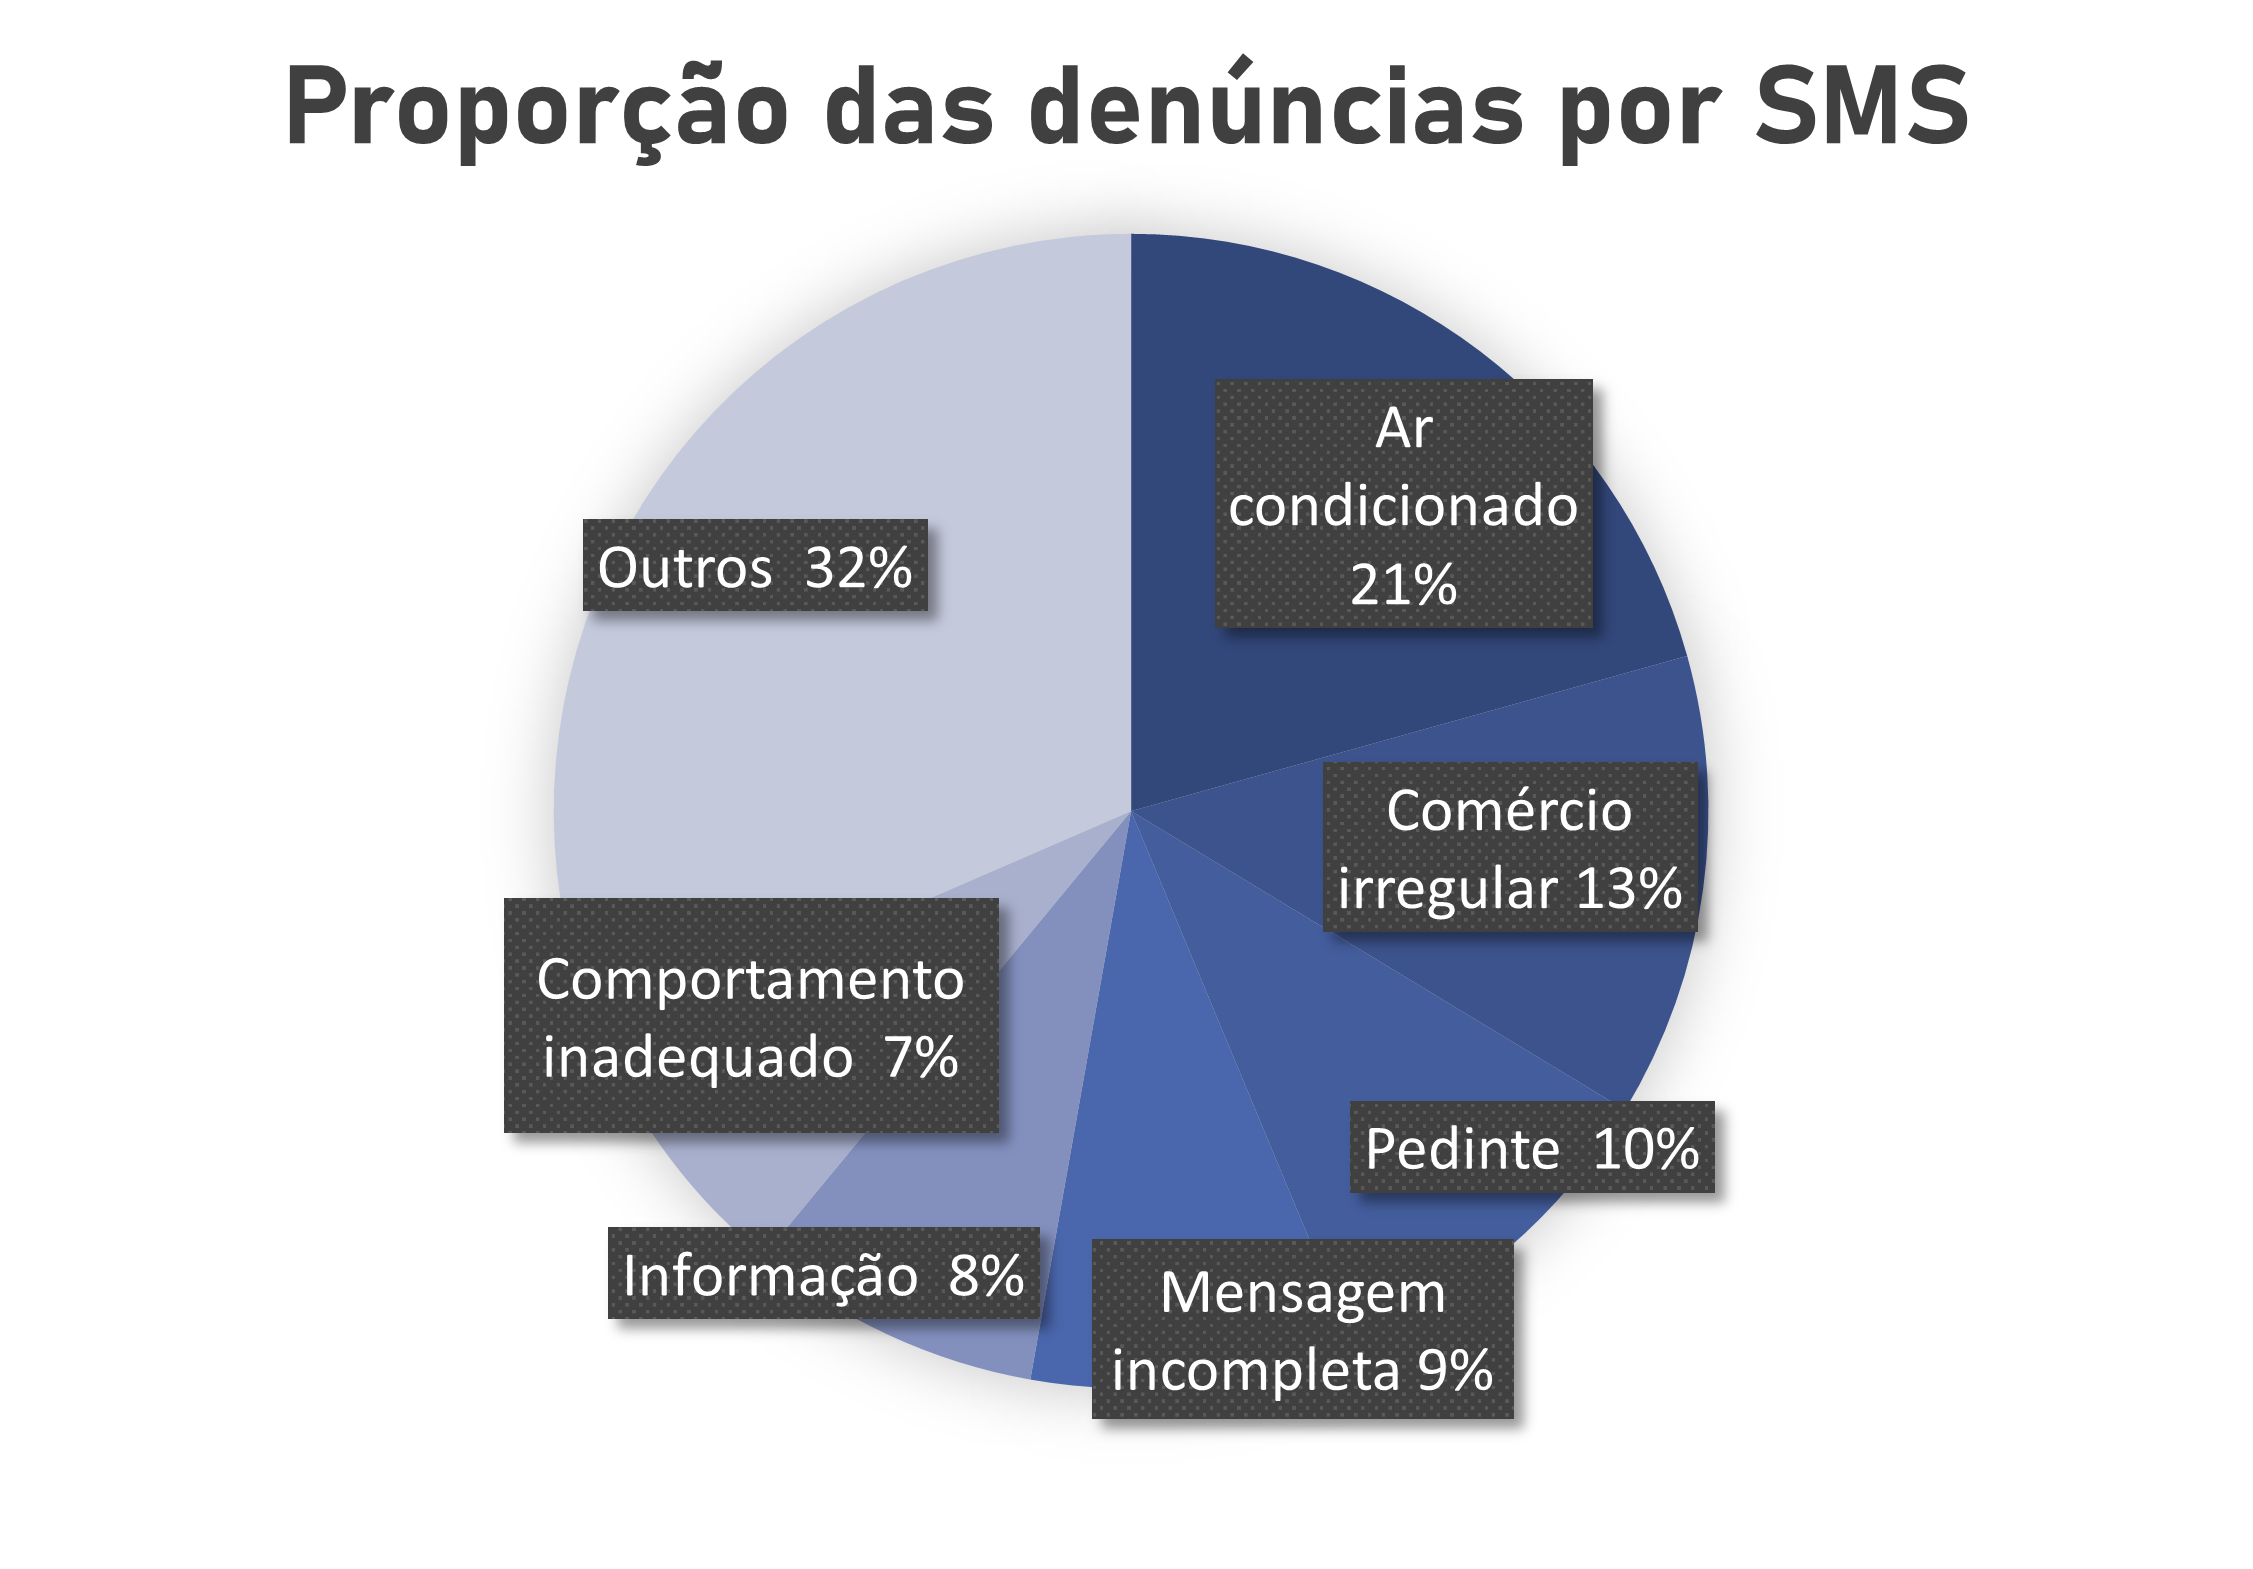
\includegraphics[width=\linewidth, height=6cm]{Imagens/Grafico_reclamacoes_totais.png}
		\smallcaption{Fonte: \textcite{metrosp2024}.}
		\label{fig:grafico_total}
	\end{minipage}\hfill
	\begin{minipage}{0.45\textwidth}
		\caption{Reclamações de ar-condicionado do Metrô de São Paulo no ano de 2023}
		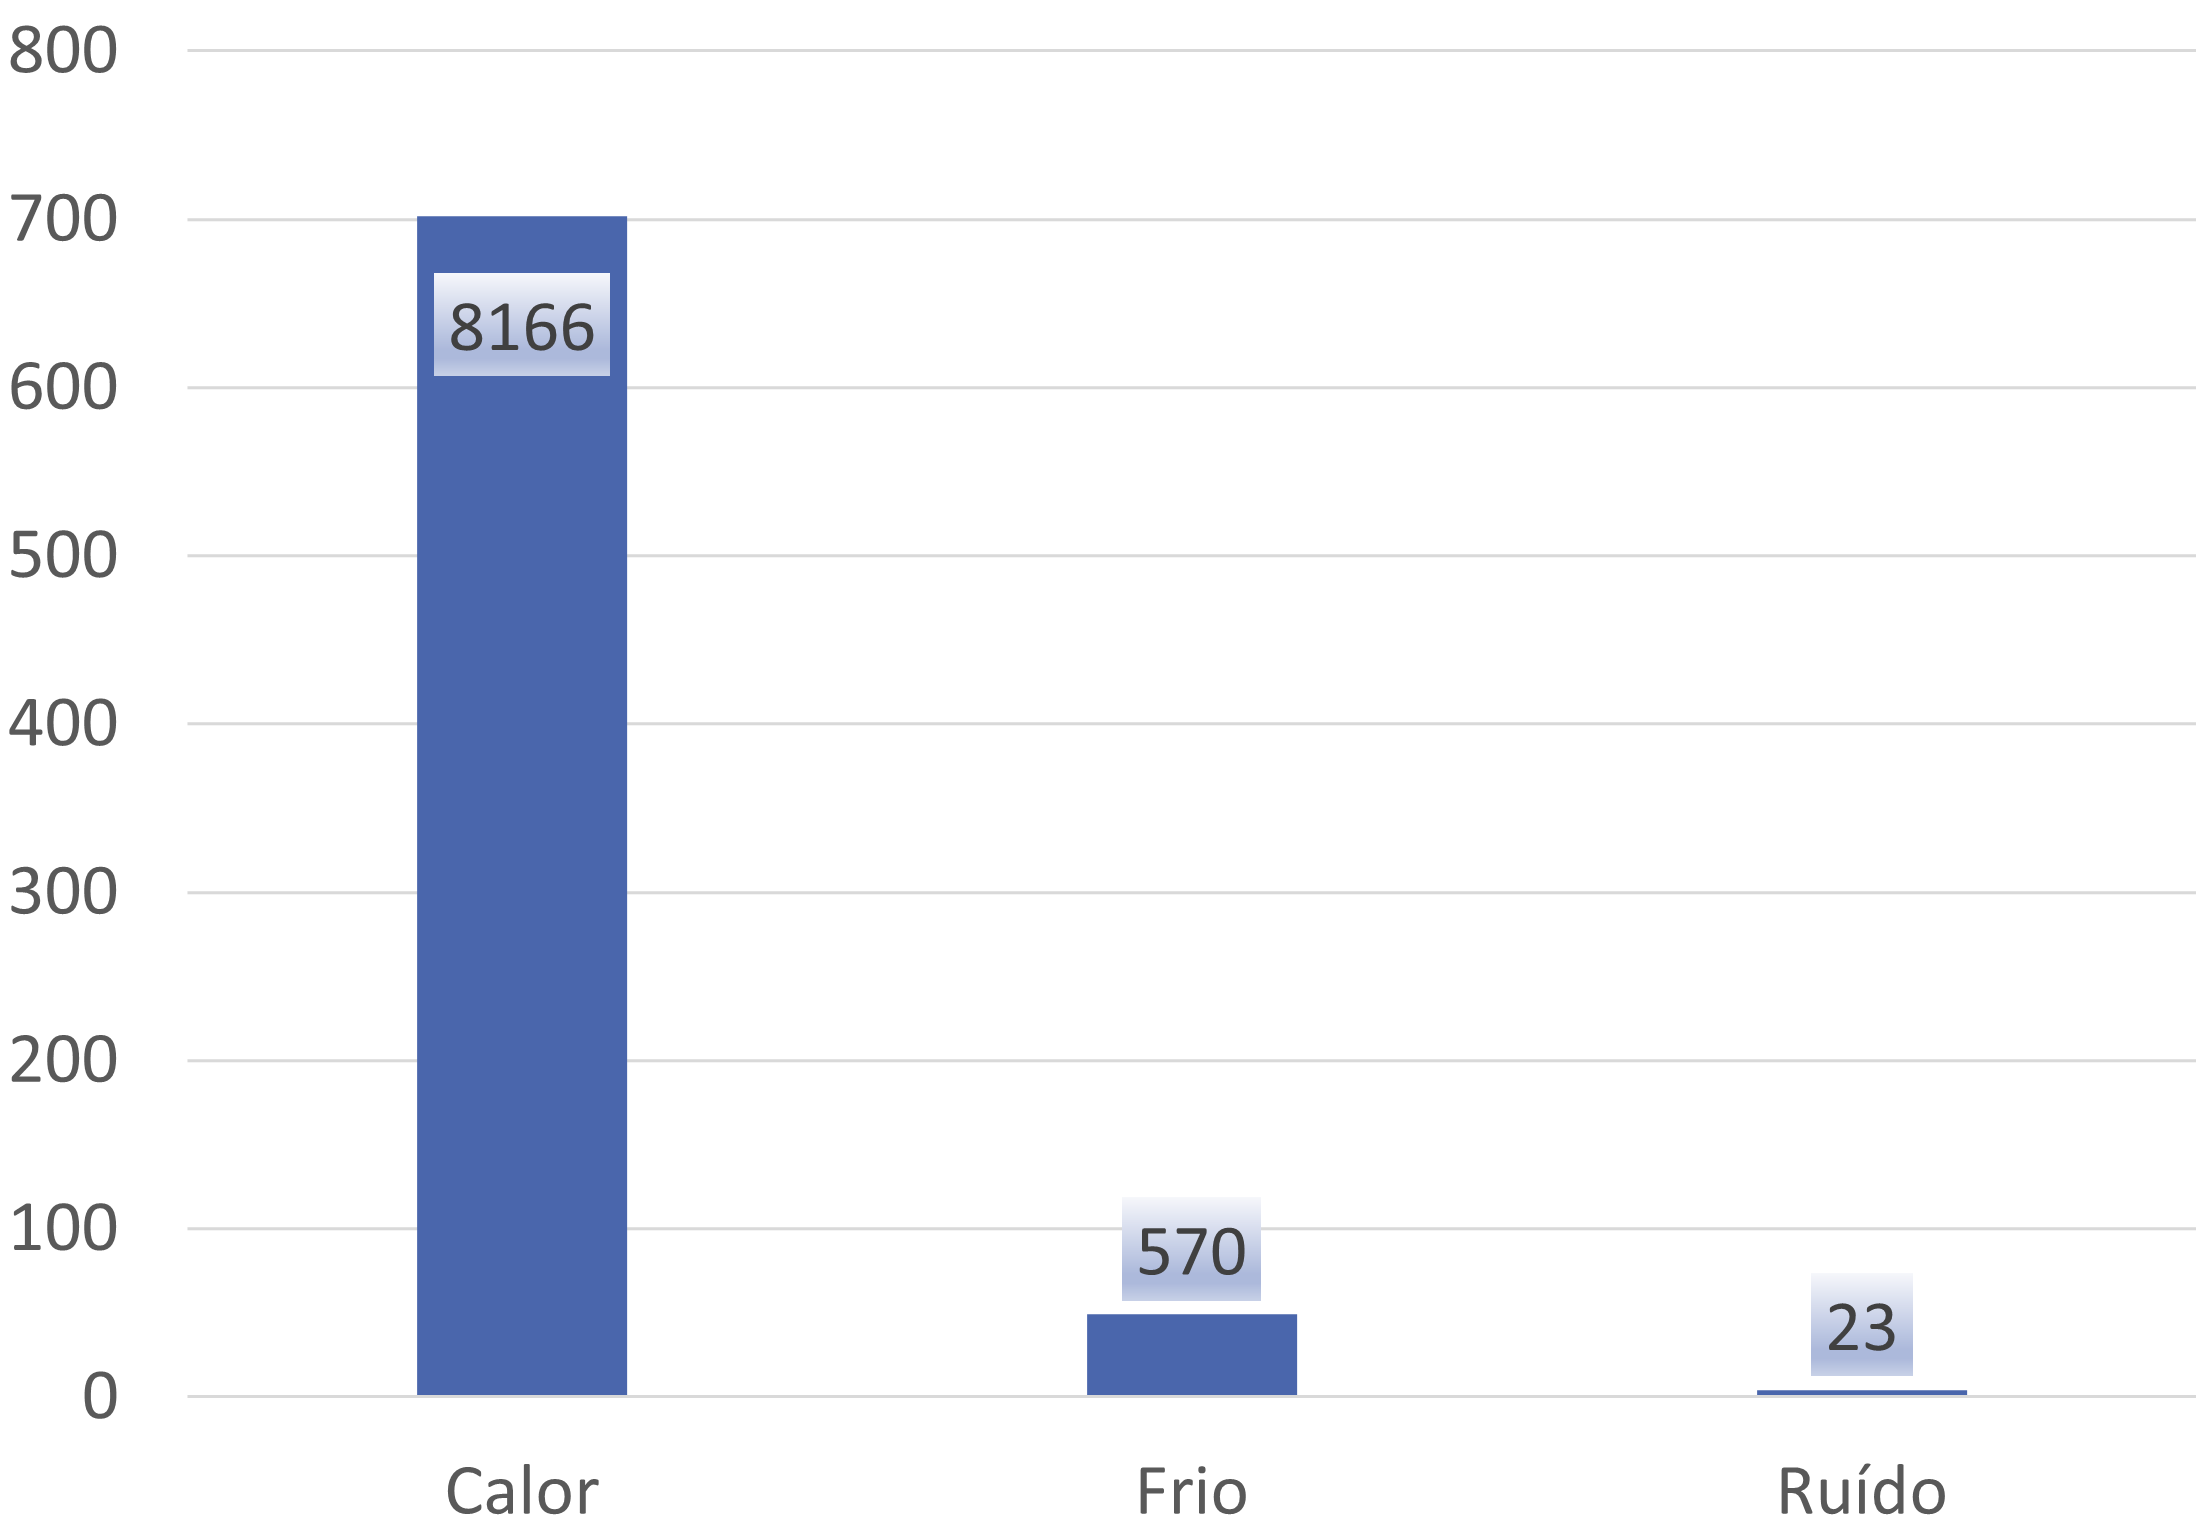
\includegraphics[width=\linewidth, height=6cm]{Imagens/Grafico_reclamacoes_ar.png}
		\smallcaption{Fonte: \textcite{metrosp2024}.}
		\label{fig:grafico_ar}
	\end{minipage}
\end{figure}

\newpage 

\section{Objetivo Geral}

O objetivo deste trabalho é realizar, através de dados de sensoriamentos no interior de um dos carros do Metrô da Frota L, uma análise do condicionamento de ar e do conforto térmico dos passageiros, entendendo assim quais são os parâmetros que influenciam suas experiências. Pretende-se correlacionar os dados obtidos e recebidos com as reclamações do canal de denúncias do Metrô via \textit{SMS}, visando compreender a percepção dos passageiros de forma qualitativa. Além disso, foi realizada a avaliação das condições térmicas dos carros e sua conformidade com as normas, se apoiando nos cálculos teóricos realizados para que se possam sugerir melhorias e oportunidades para estudos futuros. 

\section{Objetivos Específicos}

\begin{itemize}
    \item[1 -]Reunião com a equipe do Metrô de São Paulo para alinhamento de ideias e posteriormente a  aquisição dos dados relevantes para o trabalho, tais como: reclamações via \textit{SMS}, estatísticas a respeito do Metrô de São Paulo, desenhos do equipamento de Ventilação e Ar-condicionado (VAC), peso dos carros e temperaturas ao longo do tempo;
    \item[2 -]Início do tratamento e análise de dados oferecidos pelo Metrô de São Paulo, cálculos teóricos de acordo com as normas;
    \item[3 -]Desenvolvimento de placas de sensoriamento com base em \textit{Arduino}, posicionadas em locais estratégicos do carro, visando medir propriedades adicionais a serem observadas, tais como: temperatura, umidade, concentração de gás carbônico e pressão barométrica;
    \item[4 -]Visita técnica ao Metrô de São Paulo, buscando estudar o melhor posicionamento dos sensores mencionados, evitando, desta forma, desvios na aquisição dos dados;
    \item[5 -]Coleta, interpretação e análise detalhada dos dados da instrumentação;
    \item[6 -]Estudo adicional realizado através do \textit{Software Ansys}, visando melhor visualização dos dados e do comportamento do sistema;
    \item[7 -]Comparação de todos os dados coletados, calculados e tratados para uma análise completa do condicionamento de ar e do conforto térmico dos passageiros e observar se há conformidade com as normas;
    \item[8 -]Possíveis sugestões de melhoria para o sistema.
\end{itemize}

\section{Estrutura da Monografia} %REESCREVER  NO FINAL DE TUDO

No Capítulo 2 é feito o estudo do referencial teórico das normas para conforto térmico e toda a teoria que ela carrega consigo, além dos conceitos de análises computacionais. No Capítulo 3 é apresentada a metodologia do trabalho, onde estão descritas as coletas de dados, os sensores utilizados, os testes, as simulações e os cálculos a serem realizados. No Capítulo 4 são demonstrados os resultados de cada uma das áreas do projeto. No Capítulo 5 são elaboradas as conclusões cruzando os resultados de cada área do trabalho e buscando encontrar correlações. O Capítulo 6 finaliza o trabalho com as possibilidades de trabalhos futuros a partir do que foi desenvolvido.

\chapter{Referências Bibliográficas}

Para se conseguir um ambiente termicamente agradável é necessário avaliar alguns parâmetros e condições do ar. Para isso, leva-se em consideração a ventilação, as trocas de calor com o ambiente, as produções de energia térmica, os contaminantes e as taxas metabólicas. Portanto, aplicam-se balanços de energia para se calcular o conforto térmico no espaço.

\section{Leis Fundamentais da Termodinâmica} 

As leis fundamentais da termodinâmica buscam descrever as características e transformações da energia. Neste contexto, a Primeira Lei da Termodinâmica refere-se à conservação da energia, isto é, em uma interação, a energia pode alterar sua forma, porém, a quantidade total permanece a mesma e, portanto, a energia não pode ser criada ou destruída \cite{cengel1998heat}. Dessa maneira, a variação de energia é descrita como uma subtração entre a quantidade de entrada e saída no sistema, visto na Equação \ref{eq: energia}.

\begin{equation} \label{eq: energia}
    \begin{aligned}
    \Delta E = E_{\text{entrada}} - E_{\text{saída}}
    \end{aligned}
\end{equation}


Por sua vez, a Segunda Lei da Termodinâmica determina que o fluxo de calor direciona-se do corpo de temperatura mais alta para o de menor temperatura \cite{cengel1998heat}, além de incorporar o conceito de rendimento, no qual máquinas são incapazes de converter todo o calor em trabalho útil.

\section{Mecanismos de Transferência de Calor} 

A transferência de calor refere-se ao modo como o calor é transmitido entre os meios e pode ocorrer de três formas distintas, sendo elas: condução, convecção e radiação.

Em gases e líquidos, a condução ocorre através da colisão entre moléculas durante seu movimento aleatório, ao passo que, em sólidos, a mesma se dá pela vibração das moléculas, transportando energia pelos elétrons livres \cite{cengel1998heat}. A taxa de transferência de calor por condução ($\dot{Q}_{cond}$) pode ser determinada através da Lei de Fourier conforme a Equação \ref{eq:Condução}.

\begin{equation} \label{eq:Condução}
\begin{aligned}
    \dot{Q}_{\text{cond}} = k_{t} \cdot A_{\text{cond}} \cdot \frac{\Delta T}{\Delta x}
\end{aligned}
\end{equation}

Dessa maneira, o gradiente de temperatura ($\Delta T$) e a espessura da camada a ser atravessada ($\Delta x$) se relacionam à condutividade térmica do material ($k_{t}$) e área normal à direção da transferência de calor ($A_{cond}$). Entretanto, pode-se considerar uma resistência à condução do material, representada na Equação \ref{eq:Rcondução}.

\begin{equation} \label{eq:Rcondução}
\begin{aligned}
    {R}_{k}=\frac{\Delta x}{k_{t} \cdot A_{\text{cond}}}
\end{aligned}
\end{equation}

Assim, a Equação \ref{eq:Condução} pode ser reescrita conforme a Equação \ref{eq:Condução_Req}:

\begin{equation} \label{eq:Condução_Req}
\begin{aligned}
    \dot{Q}_{\text{cond}} = \frac{\Delta T}{{R}_{k}}
\end{aligned}
\end{equation}

A Tabela \ref{tab:Condutividade_Termica} indica a condutividade térmica de alguns materiais comumente utilizados no cotidiano.

\begin{table}[!htb] 
 \centering
    \caption{Condutividade térmica de materiais à temperatura ambiente}
    
\includegraphics[width=0.4\linewidth]{Tabelas/Condutividade_Termica.png}
    \smallcaption{Fonte: Autor. Adaptado de \textcite{ccengel2008heat}.}
    \label{tab:Condutividade_Termica}
\end{table}

Já a convecção trata-se da transferência de energia entre uma superfície sólida e o líquido ou gás adjacente à superfície. Assim, pode-se classificar a convecção como natural, quando ocorre devido à diferença de densidades ocasionada pela disparidade de temperaturas, ou como forçada, que, por sua vez, envolve meios externos para provocar o escoamento do fluido ao longo da superfície \cite{kreith1999mechanical}. A taxa de transferência de calor por convecção ($\dot{Q}_{conv}$) pode ser determinada através da Lei de Resfriamento de Newton conforme Equação \ref{eq:Convecção}.

\begin{equation} \label{eq:Convecção}
\begin{aligned}
    \dot{Q}_{conv}=h \cdot A_{s} \cdot (T_{s}-T_{f})
\end{aligned}
\end{equation}

Deste modo, tem-se o coeficiente de transferência de calor por convecção ($h$) multiplicado pela área da superfície na qual ocorre a troca de calor ($A_{s}$) e pela diferença entre as temperaturas da superfície ($T_{s}$) e do fluido ao longe ($T_{f}$), o qual se encontra distante o suficiente para não realizar trocas de calor por condução. Pelo mesmo raciocínio utilizado anteriormente, pode-se determinar uma resistência à convecção conforme Equação \ref{eq:Rconvecção}.

\begin{equation} \label{eq:Rconvecção}
\begin{aligned}
    {R}_{c}=\frac{1}{h \cdot A_{s}}
\end{aligned}
\end{equation}

E, portanto, a Equação \ref{eq:Convecção} pode ser reescrita como a Equação \ref{eq:Convecção_Req}:

\begin{equation} \label{eq:Convecção_Req}
\begin{aligned}
    \dot{Q}_{conv}=\frac{T_{s}-T_{f}}{{R}_{c}}
\end{aligned}
\end{equation}

Vale ressaltar que o cálculo do coeficiente de convecção depende de alguns fatores como tipo de escoamento, geometria do corpo, área de escoamento e propriedades físicas do fluido \cite{ozicsik1993heat}. Considerando-se convecção forçada em placas planas, na qual se tem um fluxo de ar paralelo a uma superfície, deve-se primeiro estabelecer o número de Nusselt que, por sua vez, está atrelado ao número de Reynolds e Prandtl. O número de Reynolds em um determinado ponto $x$ ao longo do escoamento na placa é descrito conforme Equação \ref{eq:Reynolds}, na qual $\rho$ representa a densidade do fluido, $V$ a velocidade, e $\mu$ a viscosidade dinâmica.

\begin{equation} \label{eq:Reynolds}
\begin{aligned}
    {Re}_{x}=\frac{\rho \cdot V \cdot x}{\mu}
\end{aligned}
\end{equation}

Já o número de Prandtl refere-se a uma grandeza adimensional, relacionando a espessura relativa da velocidade e das camadas limite térmicas \cite{cengel1998heat}. A Tabela \ref{tab: Propriedades_Ar} demonstra valores usuais de propriedades do ar utilizados nos cálculos de Reynolds, além do número de Prandtl de acordo com a temperatura do ar.

\begin{table}[!htb] 
 \centering
    \caption{propriedades do ar a 1 atm}
    
\includegraphics[width=0.7\linewidth]{Tabelas/Propriedades_ar_1atm.png}
    \smallcaption{Fonte: Autor. Adaptado de \textcite{ccengel2008heat}.}
    \label{tab: Propriedades_Ar}
\end{table}

\newpage

Considerando-se escoamento laminar, no qual Reynolds é menor que $5 \cdot 10^5$, pode-se determinar o número médio de Nusselt ao longo de toda a placa de comprimento $L$ conforme a Equação \ref{eq:Nusselt_Laminar}.

\begin{equation} \label{eq:Nusselt_Laminar}
\begin{aligned}
    Nu=0,664 \cdot Re_{L}^{0,5} \cdot Pr^{1/3}
\end{aligned}
\end{equation}

Para o escoamento turbulento, representado por Reynolds entre $5 \cdot 10^5$ e $10^7$ e Prandtl entre $0,6$ e $60$, o cálculo é representado pela Equação \ref{eq:Nusselt_Turbulento}.

\begin{equation} \label{eq:Nusselt_Turbulento}
\begin{aligned}
    Nu=0,037 \cdot Re_{L}^{0,8} \cdot Pr^{1/3}
\end{aligned}
\end{equation}

Dessa maneira, o coeficiente de convecção médio ao longo da placa pode ser descrito conforme Equação \ref{eq:coef. convecção}, na qual $k_{f}$ representa a condutividade térmica do fluido na média de temperatura entre a superfície e do fluido ao longe.

\begin{equation} \label{eq:coef. convecção}
\begin{aligned}
    h=\frac{k_{f} \cdot Nu}{L}
\end{aligned}
\end{equation}

Por fim, a radiação está atrelada à emissão de energia através de ondas eletromagnéticas. Vale ressaltar que todos os corpos com temperatura acima do zero Kelvin emitem radiação térmica \cite{kreith1999mechanical}. Neste contexto, sucedem os conceitos de emissividade ($\epsilon$) e absortividade ($\alpha$), os quais se referem a medidas, determinadas entre zero e um, da capacidade de um corpo de emitir e absorver radiação, respectivamente. Assim, um corpo negro apresenta valor equivalente a 1 tanto para emissividade quanto para absortividade e, portanto, representa uma situação ideal, emitindo radiação na taxa máxima, assim como absorvendo toda a radiação que incide sobre ele. 

Para situações em que a vizinhança possui dimensões muito maiores que a superfície e os meios são separados por um gás que não interfere na radiação, a taxa de transferência de calor por radiação ($\dot{Q}_{rad}$) pode ser definida pela Equação \ref{eq:Radiação}.

\begin{equation} \label{eq:Radiação}
\begin{aligned}
    \dot{Q}_{rad}=\epsilon \cdot \sigma \cdot A_{s} \cdot (T_{s}^4-T_{viz}^4)
\end{aligned}
\end{equation}

Nota-se que a determinação da radiação envolve a constante de Stefan-Boltzmann ($\sigma$), assim como as características da superfície e a temperatura da vizinhança ao seu redor ($T_{viz}$). Por sua vez, a resistência à radiação é determinada conforme Equação \ref{eq:Rradiação_R}.

\begin{equation} \label{eq:Rradiação_R}
\begin{aligned}
    {R}_{r}=\frac{1}{h_{rad} \cdot A_{s}}
\end{aligned}
\end{equation}

Na qual o coeficiente de radiação ($h_{rad}$) refere-se a uma simplificação, na Equação \ref{eq:h_rad}:

\begin{equation} \label{eq:h_rad}
\begin{aligned}
    {h}_{rad}=\epsilon \cdot \sigma \cdot (T_{s}^2+T_{viz}^2) \cdot (T_{s}+T_{viz})
\end{aligned}
\end{equation}

Logo, a Equação \ref{eq:Radiação_Req} pode ser reescrita:

\begin{equation} \label{eq:Radiação_Req}
\begin{aligned}
    \dot{Q}_{rad}=\frac {T_{s}-T_{viz}}{{R}_{r}}
\end{aligned}
\end{equation}

Um termo importante no conceito de transferência de calor refere-se ao coeficiente global de transferência de calor ($\overline{U}$), derivado de uma modificação da Lei de Resfriamento de Newton \cite{kreith1999mechanical}, conforme Equação \ref{eq:Q_Global}.

\begin{equation} \label{eq:Q_Global}
\begin{aligned}
    \dot{Q}=\overline{U} \cdot A \cdot \Delta T
\end{aligned}
\end{equation}

A Equação \ref{eq:coef. U} especifica o cálculo usualmente utilizado para obter o coeficiente global de transferência de calor, envolvendo a combinação das resistências térmicas do sistema, as quais resultam em uma resistência térmica equivalente ($R_{eq}$).

\begin{equation} \label{eq:coef. U}
\begin{aligned}
    \overline{U} \cdot A=\frac{1}{R_{eq}}
\end{aligned}
\end{equation}

E, portanto, a Equação \ref{eq:Q_Global} pode ser reescrita na Equação \ref{eq:Q_Req}:

\begin{equation} \label{eq:Q_Req}
\begin{aligned}
    \dot{Q}=\frac{\Delta T}{R_{eq}}
\end{aligned}
\end{equation}

Deste modo, assemelhando-se à elétrica, resistências térmicas em série referem-se a um sentido sequencial de fluxo de calor, ao passo que as associações em paralelo se caracterizam por um fluxo de calor que se divide. Assim, as equações de resistências equivalentes em série e paralelo são determinadas nas Equações \ref{eq:Req_serie} e \ref{eq:Req_paralelo}, respectivamente, sendo $n$ o número de resistências presentes no sistema.

\begin{equation} \label{eq:Req_serie}
\begin{aligned}
    {R}_{eq(serie)}=\sum^{n}_{i=1}{R_{i}}
\end{aligned}
\end{equation}

\begin{equation} \label{eq:Req_paralelo}
\begin{aligned}
    \frac{1}{R_{eq(paralelo)}} = \sum_{i=1}^{n} \frac{1}{R_i}
\end{aligned}
\end{equation}

Neste contexto, vale notar que nem sempre a determinação da resistência é um processo simples, especialmente para a convecção, uma vez que a velocidade do fluido e a temperatura da superfície podem ser difíceis de se obter. A norma \textcite{abnt15220} estabelece valores usuais de resistência térmica para camadas de ar em diferentes casos. A Tabela \ref{tab:Req_NBR15220} determina valores usuais de resistência para ambientes internos ($R_{si}$) e externos ($R_{se}$) ao passo que a Tabela \ref{tab:Req_Camaras} refere-se a câmaras de ar não ventiladas.

\begin{table}[!htb] 
 \centering
    \caption{Valores médios recomendados para resistência térmica superficial interna e externa}
    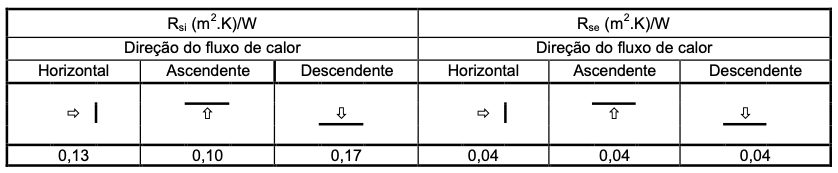
\includegraphics[width=1.0\linewidth]{Tabelas/Req_Interna_NBR15220.png}
    \smallcaption{Fonte: \textcite{abnt15220}.}
    \label{tab:Req_NBR15220}
\end{table}

\begin{table}[!htb] 
 \centering
    \caption{Valores médios recomendados para resistência térmica em câmaras de ar não ventiladas, com largura muito maior que a espessura}
    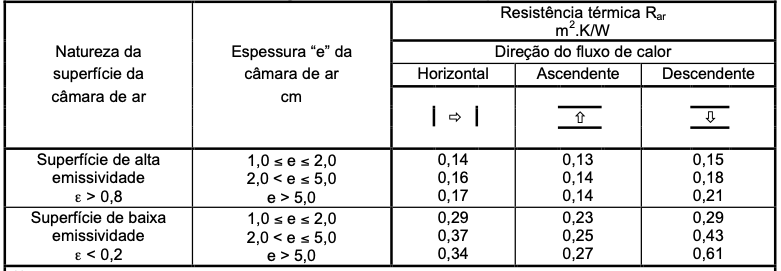
\includegraphics[width=1.0\linewidth]{Tabelas/Req_CamaraAr_NBR15220.png}
    \smallcaption{Fonte: \textcite{abnt15220}.}
    \label{tab:Req_Camaras}
\end{table}

\newpage

\section{Balanço de Energia} \label{balenergia}

O balanço de energia representa o comportamento do fluxo de calor em um sistema. Neste contexto, a energia interna ($U$) é a somatória das formas de energia microscópicas de um sistema, sendo representada pelas energias cinética e potencial das moléculas \cite{cengel1998heat}. Vale ressaltar que, ao se considerar um regime permanente, a variação da energia ao longo do tempo equivale a zero.

A energia interna está relacionada com as forças intermoleculares que, portanto, unem as moléculas. Assim, a porção cinética de energia refere-se ao calor sensível, ao passo que o calor latente está atrelado à mudança de fase. Dessa maneira, observando-se um ambiente climatizado, pode-se afirmar que o calor sensível está relacionado à temperatura, enquanto o calor latente à umidade do local.

Considerando-se um sistema de fluxo constante, no qual não ocorrem mudanças expressivas nas energias cinética e potencial, e sem a parcela de trabalho, a taxa de transferência de calor sensível ($\dot{Q}_{S}$) sendo adicionado ou retirado de um sistema é representada pela Equação \ref{eq:Qsensível}, na qual $\dot{m}$ representa a vazão mássica, $\Delta{T}$ equivale à diferença de temperatura e ${Cp}$ é o calor específico do ar à pressão constante, para o qual \textcite{cengel1998heat} considera $1,007 \space kJ/kg K$ à temperatura de $20^\circ C$ e $1 \space atm$. 

\begin{equation} \label{eq:Qsensível}
\begin{aligned}
    \dot{Q}_{S}=\dot{m} \cdot \Delta{h}= \dot{m} \cdot Cp \cdot \Delta{T}
\end{aligned}
\end{equation}

Entretanto, vale ressaltar que a diferença de temperaturas pode ser utilizada apenas para o calor sensível, uma vez que durante a mudança de fase a temperatura permanece constante. Logo, para a análise da taxa de transferência de calor latente ($\dot{Q}_{L}$), pode-se realizar uma comparação da umidade absoluta ($W$) conforme Equação \ref{eq:Qlatente}, na qual $L$ corresponde ao calor latente de vaporização da água e é definida como $2501 \space kJ/kg$ pela \textcite{abnt16655}.

\begin{equation} \label{eq:Qlatente}
\begin{aligned}
    \dot{Q}_{L}=\dot{m} \cdot \Delta{h}= \dot{m} \cdot L \cdot \Delta{W}
\end{aligned}
\end{equation}

Neste contexto, torna-se importante destacar a influência das pessoas no calor sensível e latente do ambiente. A Tabela \ref{tab:Metabolismo_ashrae} demonstra taxas representativas destas variáveis liberadas pelo ser humano em diferentes níveis de atividade.

\begin{table}[!htb] 
 \centering
    \caption{Taxas Representativas de Calor Sensível e Latente Liberados pelo Ser Humano em Diferentes Níveis de Atividade}
    
\includegraphics[width=1.0\linewidth]{Tabelas/Metabolismo_ashrae.png}
    \smallcaption{Fonte: Autor. Adaptado de \textcite{handbook2017ashrae}.}
    \label{tab:Metabolismo_ashrae}
\end{table}

Outro fator de influência no calor sensível refere-se à iluminação do local. A Tabela \ref{tab:LPD} estabelece valores máximos da densidade de potência da luz, em inglês, \textit{Light Power Density} \textit{(LPD)}, para diferentes locais, representando a carga térmica da iluminação baseada na área atingida pela luz.

\begin{table}[!htb] 
 \centering
    \caption{Densidade de potência da luz para diferentes locais}
    
\includegraphics[width=0.5\linewidth]{Tabelas/LPD.png}
    \smallcaption{Fonte: Autor. Adaptado de \textcite{ashrae2013ashrae}.}
    \label{tab:LPD}
\end{table}

\newpage

Além disso, equipamentos presentes no local também contribuem para a carga térmica sensível do sistema. A Tabela \ref{tab:Qs_Monitores} refere-se à influência de monitores no ganho de calor do ambiente.

\begin{table}[!htb] 
 \centering
    \caption{Carga térmica de diferentes monitores}
    
\includegraphics[width=0.5\linewidth]{Tabelas/Qs_Monitores.png}
    \smallcaption{Fonte: Autor. Adaptado de \textcite{sarfraz2018experimental}.}
    \label{tab:Qs_Monitores}
\end{table}

Dessa maneira, as fontes de geração ou retirada de calor sensível e latente devem ser somadas a fim de realizar uma análise fundamentada de carga térmica do sistema. 

\section{Ventilação} \label{ventilação}

Por definição, ventilação é um processo no qual se retira ou fornece ar por meios mecânicos, de ou para um ambiente fechado, com o objetivo de purificar, controlar a distribuição, a temperatura e a umidade do ar dentro do recinto. A ventilação utilizada foi a Ventilação Geral Diluidora (VGD). 

A VGD se trata de um sistema para captura do contaminante no ar quando este já não se encontra mais na fonte que o gerou. Segundo \textcite{ventilacaoindustrial} a VGD deve manter o conforto e eficiência do homem, garantir a saúde e segurança do ser humano e conservar em bom estado os equipamentos e materiais utilizados no ambiente.

Uma VGD é composta por um sistema de captação externa, filtro, ventilador de insuflamento, ventilador de exaustão, dutos, bocas de insuflamento e de exaustão e a descarga de ar viciado.

Existem quatro maneiras de instalação e configuração de uma VGD, a depender da situação em que o ambiente se encontra. Elas são: insuflamento e exaustão naturais; insuflamento mecânico e exaustão natural; insuflamento natural; exaustão mecânica e insuflamento e exaustão mecânicos \cite{ventilacaoindustrial}.

A VGD tem a função de captar contaminantes no ar para que eles não sejam absorvidos pelo corpo humano. Sabendo disso, existem concentrações adequadas de contaminantes gasosos no ar e elas podem ser calculadas através da Equação \ref{eq:cont}.

\begin{equation} \label{eq:cont}
    \begin{aligned}
C=\frac{n_{Contam.}}{n_{Total}}=\frac{V_{Contam.}}{V_{Total}}
    \end{aligned}
\end{equation}

A ventilação também deverá introduzir uma vazão de ar novo no ambiente, e o fluxo de ar que sai leva embora os contaminantes diluídos. 

Portanto, a vazão de ar novo é necessária para suprir os níveis de ${O}_{2}$, manter adequado o nível de ${CO}_{2}$ e diluir odores, manter temperatura, umidade, diluir contaminantes e manter a velocidade do ar confortável. Para isso, existem cálculos, que foram demonstrados mais à frente, para que a vazão de ar novo cumpra todas as necessidades do ambiente.

Para que os níveis de ${O}_{2}$ e ${CO}_{2}$ e odores fiquem aceitáveis, a ANVISA e a \textcite{abnt216401}. sugerem que a vazão de ar novo mínima necessária siga a Equação \ref{eq:anvisa}.

\begin{equation} \label{eq:anvisa}
\begin{aligned}
    \dot{V}_{ArNovo}=N_{Pessoas}\cdot {\dot{V}_{Pessoa}}
\end{aligned}
\end{equation}

Sendo $N_{Pessoas}$ o número de pessoas no ambiente e $\dot{V}_{Pessoas}$ a vazão mínima por pessoa. Sendo esse último valor definido pela ANVISA, é recomendado usar $27$ $m^3/(h\cdot{pessoa}$).

Para que a temperatura seja mantida, a vazão de ar novo a ser colocada no ambiente é descrita na Equação \ref{eq:tempV}.

\begin{equation} \label{eq:tempV}
\begin{aligned}
    \dot{V}_{ArNovo}=\frac{\dot{m}_{ArNovo}}{\rho_{ArNovo}}
\end{aligned}
\end{equation}

Os níveis de odores, fumaças e contaminantes precisam ser diluídos e para isso a vazão de ar novo necessária é descrita na Equação \ref{eq:contam.}.

\begin{equation} \label{eq:contam.}
    \begin{aligned}
     \dot{V}_{ArNovo}=\frac{\dot{q}}{C_{Eq.}-C_{Insufl.}}
    \end{aligned}
\end{equation}

Ou quando não se dilui completamente os contaminantes tem-se a Equação \ref{eq:contam.K}.

\begin{equation} \label{eq:contam.K}
    \begin{aligned}
\dot{V}_{\text{ArNovo}} = K \cdot \frac{\dot{q}}{C_{\text{Máx.}} - C_{\text{Insufl.}}}
   \end{aligned}
\end{equation}

$K$ é um coeficiente de segurança que varia de $3$ a $10$.

Manter a velocidade do ar conveniente é importante para o conforto e o ideal é que ela esteja entre $0,1$ $m/s$ e $1,2$ $m/s$. Pode ser medida utilizando a vazão e a área do ambiente, como visto na Equação \ref{eq:veloc}.

\begin{equation} \label{eq:veloc}
\begin{aligned}
   \dot{V}_{ArNovo}=v\cdot{A}
\end{aligned}
\end{equation}

\section{Conforto térmico} \label{confortotermico}

Segundo a \textcite{ASHRAE2009}, conforto térmico é a condição mental que expressa satisfação com o ambiente térmico e é uma avaliação subjetiva. Mas, se $80\%$ das pessoas de um ambiente estiverem confortáveis, é possível dizer que há conforto térmico.

De acordo com \textcite{konstantinov2015numerical}, o conforto térmico dos passageiros se tornou um critério de design importante para os fabricantes de trens. Isso porque, apesar de as sensações individuais serem bem diferentes umas das outras, elas dependem do fluxo de ar, da distribuição de temperatura dentro do ambiente e da radiação de calor na cabine. É por essa questão que o estudo de conforto térmico foca na ventilação e qualidade do ar.

Com base em estudo realizado por \textcite{casellisimulaccao}, um carro de trem se encontra em diferentes situações em relação à troca de calor do ambiente, portanto, existe um índice que representa um nível aceitável de conforto térmico para as pessoas. Esse índice depende de alguns parâmetros físicos, processos fisiológicos, psicológicos e culturais. 

Em pesquisas anteriores de \textcite{TCCThomas}, tem-se uma análise comparativa do conforto térmico entre as linhas vermelha e azul do Metrô de São Paulo, na qual sensores de temperatura e umidade foram dispostos no interior de um carro da linha vermelha durante o trajeto de ida e volta usualmente percorrido pelo mesmo. Dessa maneira, a coleta de dados ocorreu das 16h08 às 17h29, e foi comparada com simulações realizadas no \textit{software} \textit{Ansys Fluent}, além de avaliar em relação à norma existente \textcite{handbook2006american}. Deste modo, foi notada uma influência do fluxo de passageiros na temperatura e umidade no interior dos carros, uma vez que o percurso de retorno, o qual possui maior fluxo de pessoas, apresentou gradiente de temperatura acima do especificado pela norma ao longo de grande parte do trajeto. Além disso, o estudo resultou em uma disparidade de temperatura e velocidade do ar entre a norma e a simulação tanto para os carros da linha azul quanto aos da linha vermelha.

\subsection{Balanço de energia do corpo} \label{balancocorpo}

Para que seja possível avaliar o conforto térmico, é preciso fazer um balanço de energia baseado na taxa de produção de calor metabólico $(M [W/m^{2}])$ e na taxa de trabalho mecânico realizado $(W [W/m^{2}])$ \cite{ASHRAE2009}. As Equações \ref{eq:energiapessoa} e \ref{eq:energiapessoa1} mostram o balanço de energia.

\begin{equation} \label{eq:energiapessoa}
    \begin{aligned}
    M - W = q_{\text{sk}} + q_{\text{res}} + S
    \end{aligned}
\end{equation}

\begin{equation} \label{eq:energiapessoa1}
    \begin{aligned}
    M - W = (C + R+ E_{\text{sk}}) + (C_{\text{res}} + E_{\text{res}}) + (S_{\text{sk}} + S_{\text{cr}})
    \end{aligned}
\end{equation}

A soma da perda de calor sensível da pele ($(C + R)$ $[W/m^{2}]$) com a taxa total da perda de calor por evaporação da pele ($E_{\text{sk}}$ [$W/m^{2}$]) formam a taxa total de calor perdido da pele ($q_{\text{sk}}$ $[W/m^{2}]$). A taxa total de calor perdido pela respiração ($q_{\text{res}}$ $[W/m^{2}]$) se dá pela soma da taxa de calor convectivo perdida pela respiração ($C_{\text{res}}$ $[W/m^{2}]$) e a taxa de calor latente perdido pela respiração ($E_{\text{res}}$ $[W/m^{2}]$). Por fim, a taxa total de armazenamento de calor (S $[W/m^{2}]$) é dada pela soma das taxas de armazenamento de calor na pele ($S_{\text{sk}}$ $[W/m^{2}]$) e de armazenamento de calor nos compartimentos internos do corpo ($S_{\text{cr}}$ $[W/m^{2}]$).


Os parâmetros apresentados nas Equações \ref{eq:energiapessoa} e \ref{eq:energiapessoa1} têm como unidade energia por área superficial do corpo nu (\textcite{ASHRAE2009}). A melhor e mais usual área superficial ($A_{D}$ $[m^{2}]$) utilizada foi elaborada originalmente por \textcite{dubois1916formula} e é mostrada na Equação \ref{eq:dubois}.

\begin{equation} \label{eq:dubois}
    \begin{aligned}
   A_{\text{D}} = 0,202 \cdot m^{0,425} \cdot l^{0,725}
    \end{aligned}
\end{equation}

Onde, $m$ é a massa da pessoa em $kg$ e $l$, a altura em $m$. 

As taxas de metabolismo (\textit{M}) tabuladas estão mostradas na Tabela \ref{tab: metabolismo} onde $1$ $met$ equivale à $58,2$ $W/m^2$.

\begin{table}[!htb] 
 \centering
    \caption{Geração de calor metabólico para variadas atividades}
    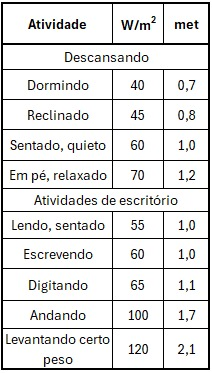
\includegraphics[width=0.4\linewidth]{Tabelas/tabela-met1.jpeg}
    \smallcaption{Fonte: Autor. Adaptado de \textcite{ASHRAE2009}.}
    \label{tab: metabolismo}
\end{table}

Porém, para medições mais apuradas do metabolismo pode-se calculá-lo através da Equação \ref{eq:metabolismo}.

\begin{equation} \label{eq:metabolismo}
    \begin{aligned}
   M = \frac{21(0,23RQ + 0,77)Q_{{O_{2}}}}{A_{D}}
    \end{aligned}
\end{equation}

Onde, \textit{M} é a taxa de metabolismo medida em $W/m^2$, \textit{RQ} é o coeficiente respiratório, no qual é a razão molar entre a quantidade de ${O}_{2}$ inalado e a quantidade de ${CO}_{2}$ expirado e é adimensional. E, por fim, $Q_{0_{2}}$ é a taxa volumétrica de consumo de oxigênio nas condições de $0^\circ C$ e $101,325$ $kPa$, medida em $mL/s$.

É importante ressaltar que a variável \textit{RQ} depende da atividade da pessoa, sua dieta e sua condição física. Ela pode ser medida calculando o fluxo de ar da expiração e da inspiração da pessoa ou pode ser estimada com certa precisão. Uma boa estimativa para um adulto comum é $RQ$ = $0,83$ para atividades do dia a dia e $RQ$ = $1$ para esforços extremamente pesados.

O oxigênio consumido é estimado através dos batimentos cardíacos e nível de esforço \cite{aastrand2003textbook}. Essas relações estão mostradas na Tabela \ref{tab: bpm e o2}.

\begin{table}[!htb] 
 \centering
    \caption{Batimentos cardíacos e consumo de oxigênio em diferentes níveis de atividade}
    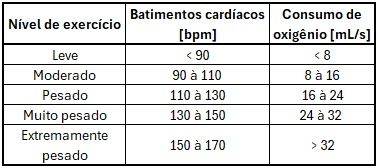
\includegraphics[width=0.5\linewidth]{Tabelas/bpm-o2.jpeg}
    \smallcaption{Fonte: Autor. Adaptado de \textcite{aastrand2003textbook}.}
    \label{tab: bpm e o2}
\end{table}

Seguindo a ordem da Equação \ref{eq:energiapessoa}, tem-se a perda de calor sensível pela pele. A troca de calor da pele tem que passar pela roupa para chegar ao ambiente. Esse caminho é feito em série e pode ser descrito em dois passos: o primeiro é da pele, para o isolamento da roupa, para a superfície da roupa, para o ambiente; o segundo é pela superfície da roupa para o ambiente \cite{ASHRAE2009}.

Tanto a convecção (\textit{C}), quanto a radiação (\textit{R}) perdidas pela superfície da roupa do corpo humano podem ser expressas em função do coeficiente de transferência de calor e a diferença de temperatura média da superfície da roupa e a temperatura apropriada do ambiente ao redor, como é visto nas Equações \ref{eq:c} e \ref{eq:r}. 

\begin{equation} \label{eq:c}
    \begin{aligned}
    C = f_{cl} h_{c} (t_{cl} - t_{a})
    \end{aligned}
\end{equation}


\begin{equation} \label{eq:r}
    \begin{aligned}
    R = f_{cl} h_{r} (t_{cl} - t_{r})
    \end{aligned}
\end{equation}

As Equações \ref{eq:c} e \ref{eq:r}, normalmente, são combinadas para expressar a troca de calor sensível total pelos dois mecanismos a partir da temperatura de operação ($t_{o}$). Mostrado na Equação \ref{eq:c+r}.

\begin{equation} \label{eq:c+r}
    \begin{aligned}
    C+R = f_{cl} h_{comb} (t_{cl} - t_{o})
    \end{aligned}
\end{equation}

Onde, $t_{o}$ é calculado pela Equação \ref{eq:to}. E o $h_{comb}$, pela Equação \ref{eq:hcomb}.

\begin{equation} \label{eq:to}
    \begin{aligned}
   t_{o}= \frac{h_{r}t_{r}+h_{c}t_{a}}{h_{r}+h_{c}}
    \end{aligned}
\end{equation}

\begin{equation} \label{eq:hcomb}
    \begin{aligned}
   h_{comb}=h_{r}+h_{c}
    \end{aligned}
\end{equation}

A temperatura de operação ($t_{o}$) é a média ponderada entre a temperatura radiante externa ($t_{r}$) e a temperatura ambiente ($t_{a}$) e seus respectivos coeficientes de transferência de calor. Já a temperatura da superfície da roupa é calculada através de uma iteração, mostrada na Equação \ref{eq:tcl}.

\begin{equation} \label{eq:tcl}
    \begin{aligned}
   t_{cl}= 35,7-0,028(M-W) - R_{cl}(39,6\cdot10^{-9}f_{cl}[(t_{cl}+273)^4-(t_{r}+273)^4]+f_{cl}h_{c}(t_{cl}-t_{a}))
    \end{aligned}
\end{equation}

Segundo a \textcite{ASHRAE2009} ambos os coeficientes $h_{c}$ e $h_{r}$ são calculados para a superfície da roupa. O coeficiente de transferência de calor por convecção é normalmente causado pelo movimento do ar no local ou por movimentos dos corpos. As equações que estimam $h_{c}$ estão apresentadas na Tabela \ref{tab: valores de hc}. 

\begin{table}[!htb] 
 \centering
    \caption{Equações para estimativa do coeficiente de transferência de calor por convecção}
    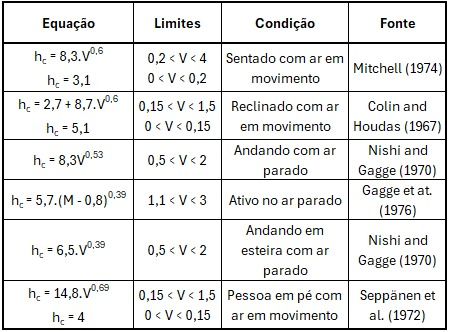
\includegraphics[width=0.5\linewidth]{Tabelas/tabela-hc.jpeg}
    \smallcaption{Fonte: Autor. Adaptado de \textcite{ASHRAE2009}.}
    \label{tab: valores de hc}
\end{table}


Já o coeficiente de transferência de calor por radiação é calculado através da Equação \ref{eq:hr}.

\begin{equation} \label{eq:hr}
    \begin{aligned}
   h_{r}=4 \epsilon \sigma \frac{A_{r}}{A_{D}}(273,2 + \frac{t_{cl}+t_{r}}{2})^3
    \end{aligned}
\end{equation}

Na qual, $\epsilon$ é a emissividade, normalmente usada 0,95 para a pele humana, $\sigma$ é a constante de Stefan-Boltzmann ($5,67\cdot10^{-8}$ $W/m^{2}K^{4}$) e $A_{r}$ é a área de radiação efetiva do corpo ($m^2$). A razão $A_{r}/A_{D}$ é 0,70 para uma pessoa sentada e 0,73 para uma pessoa em pé.

Em alguns casos, a variável $t_{cl}$ é desconhecida, portanto, não é possível calcular o $h_{r}$. Para isso, em temperaturas típicas de ambientes internos, $h_{r}$ é quase constante, podendo, assim, ser usada a aproximação vista na Equação \ref{eq:hr1}.

\begin{equation} \label{eq:hr1}
    \begin{aligned}
   h_{r}=4,7\cdot \epsilon
    \end{aligned}
\end{equation}


Um fator de correção $f_{\text{cl}}$ deve ser aplicado para que a transferência de calor da pele leve em consideração a área superficial do corpo com a resistência superficial da roupa ($I_{cl}$). A Tabela \ref{tab: valores de fcl e icl} mostra alguns valores para variados conjuntos de roupas \cite{mccullough1989data}.

\begin{table}[!htb] 
 \centering
    \caption{Valores de isolamento e permeabilidade para conjunto de roupas típicos}
    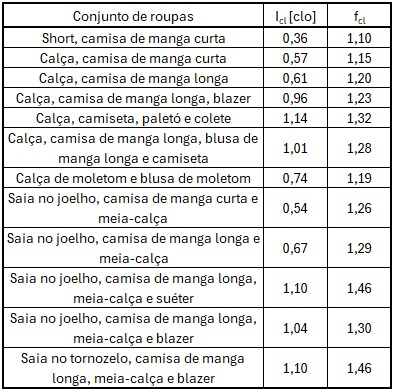
\includegraphics[width=0.5\linewidth]{Tabelas/tabela-roupas.jpeg}
    \smallcaption{Fonte: Autor. Adaptado de \textcite{mccullough1989data}.}
    \label{tab: valores de fcl e icl}
\end{table}

Na Tabela \ref{tab: valores de fcl e icl}, $I_{cl}$ está em unidade de $clo$ que corresponde a $0,155$ $m^2K/W$. Para não haver confusão quando a resistência da roupa for utilizada em $m^2K/W$ o símbolo $R_{cl}$ será usado.

Em casos em que se pode medir $f_{cl}$ e as condições são bem definidas é possível calcular $R_{cl}$ através da Equação \ref{eq:rcl}.

\begin{equation} \label{eq:rcl}
    \begin{aligned}
   R_{cl}= \frac{t_{sk}-t_{o}}{q}-\frac{1}{h\cdot f_{cl}}
    \end{aligned}
\end{equation}

Onde \textit{q} é o calor perdido do corpo em $W/m^2$ e $t_{sk}$ é a temperatura média do compartimento da pele e pode ser descrita pela Equação \ref{eq:tsk}.

\begin{equation} \label{eq:tsk}
    \begin{aligned}
   t_{sk}= 35,7 - 0,00275(M-W)
    \end{aligned}
\end{equation}

Ainda sobre a perda de calor da pele para o ambiente tem-se o calor perdido por evaporação ($E_{sk}$), mostrado na Equação \ref{eq:esk}.

\begin{equation} \label{eq:esk}
    \begin{aligned}
   E_{sk}= \frac{w(p_{sk,s}-p_{a})}{R_{e,cl}+\frac{1}{f_{cl}h_{e}}}
    \end{aligned}
\end{equation}

Na Equação \ref{eq:esk} tem-se a presença de duas pressões: a pressão de vapor d'água na pele, na temperatura $t_{sk}$ (normalmente assumido como saturado) ($p_{sk,s}$ [$kPa$]) e a pressão de vapor d'água no ambiente ($p_{a}$ [$kPa$]). Tem-se também a resistência de transferência de calor por evaporação da roupa ($R_{e,cl}$ [$m^2kPa/W$]), equivalente ao $R_{cl}$, a umidade da pele ($w$) e o coeficiente de transferência de calor por evaporação ($h_{e}$ [$W/m^2K$]).

A umidade da pele ($w$) é dada pela razão da verdadeira perda de calor por evaporação pela perda máxima de calor na qual ocorre em $E_{max}$ onde o calor perdido é máxima quando $w$ = $1$. Ela é muita relacionada com o desconforto térmico e é um ótimo medidor se as temperaturas estão muito altas. Teoricamente, a umidade da pele pode se aproximar de 1 enquanto o corpo se mantém controlado termicamente \cite{berglund1977evaporation}. \textcite{azer1982design} recomenda um valor de 0,5 para condições de pessoa saudável em um ambiente climatizado.

Com isso, tem-se a primeira parcela da equação de energia (Equação \ref{eq:energiapessoa1}), a perda total de calor pela pele ($q_{sk}$). Essa parcela pode ser escrita, também, como mostra a Equação \ref{eq:qsk}.

\begin{equation} \label{eq:qsk}
    \begin{aligned}
   q_{sk}= (C + R + E_{sk})
    \end{aligned}
\end{equation}

Após descrita a parcela da perda total de calor pela pele, tem-se a parcela de perda de calor pela respiração. Essa parcela é mostrada na Equação \ref{eq:qres}.

\begin{equation} \label{eq:qres}
    \begin{aligned}
   q_{res}= (C_{res} + R_{res})
    \end{aligned}
\end{equation}

A perda total de calor pela respiração é normalmente expressa em função de calores sensível ($C_{res}$) e latente ($E_{res}$). As Equações \ref{eq:cres} e \ref{eq:eres} são aproximações simplificadas das expressões de perdas de calor, pois a perda de calor pela respiração seca é relativamente pequena. Portanto, as equações foram utilizadas em condições normais de temperatura e umidade ($20^\circ C$ e $50\%$, respectivamente) \cite{ASHRAE2009}.

\begin{equation} \label{eq:cres}
    \begin{aligned}
   C_{res}= 0,0014M(34-t_{a})
    \end{aligned}
\end{equation}

\begin{equation} \label{eq:eres}
    \begin{aligned}
   R_{res}= 0,0173M(5,87-p_{a})
    \end{aligned}
\end{equation}

A última parcela necessária para que o balanço de energia possa ser calculado é a taxa de armazenamento de calor do corpo. Essa taxa é dividida em duas partes: a primeira é a taxa de armazenamento de calor na pele, e a segunda, a taxa de armazenamento de calor nos compartimentos internos do corpo. A taxa de armazenamento pode ser escrita separadamente para cada compartimento em termos de capacidade térmica e tempo de troca de temperatura em cada compartimento. \cite{ASHRAE2009} As Equações \ref{eq:scr} e \ref{eq:ssk} mostram as formulações das taxas. 

\begin{equation} \label{eq:scr}
    \begin{aligned}
   S_{cr}= \frac{(1-\alpha_{sk})mc_{p,b}}{A_{D}}\cdot \frac{dt_{cr}}{d\theta}
    \end{aligned}
\end{equation}

\begin{equation} \label{eq:ssk}
    \begin{aligned}
   S_{sk}= \frac{\alpha_{sk}mc_{p,b}}{A_{D}}\cdot \frac{dt_{sk}}{d\theta} 
    \end{aligned}
\end{equation}

A variável $\alpha_{sk}$ é a fração mássica do corpo concentrada no compartimento da pele (adimensional); $c_{p,b}$ é a capacidade térmica específica do corpo ($3490$ $J/(kgK)$); as temperaturas $t_{cr}$ e $t_{sk}$ são, respectivamente, a temperatura do compartimento central e da pele ($^\circ C$); $\theta$ é o tempo, em segundos.

A fração mássica do corpo ($\alpha_{sk}$) pode ser calculada por meio da Equação \ref{eq:alpha} e depende do fluxo sanguíneo na superfície da pele, $\dot{Q}_{bl}$ ($L/hm^2$), mostrada na Equação \ref{eq:qbl}.  

\begin{equation} \label{eq:alpha}
    \begin{aligned}
    \alpha_{sk}= 0,0418+ \frac{0,745}{\dot{Q}_{bl} - 0,585} 
    \end{aligned}
\end{equation}

\begin{equation} \label{eq:qbl}
    \begin{aligned}
   \dot{Q}_{bl}= \frac{BFN + c_{dil}(t_{cr-37})}{1 + S_{tr}(34-t_{sk})} 
    \end{aligned}
\end{equation}

Para uma pessoa comum os parâmetros $BFN$, $c_{dil}$ e $S_{tr}$ têm valores de $6,3$, $50$ e $0,5$, respectivamente. Um ser humano tem um $\dot{Q}_{bl}$ limitado a um máximo de $90$ $L/(hm^2)$. 

\subsection{\textit{Predicted Mean Vote (PMV)} e \textit{Predicted Percent of Dissatisfied (PPD)}}

Apesar de o conforto térmico ser subjetivo, é possível avaliá-lo através do método \textit{PMV} - \textit{PPD}, criado por \textcite{fanger1970thermal} para prever o voto de satisfação das pessoas e a porcentagem de pessoas insatisfeitas com o ambiente. \textcite{fanger1970thermal}, relacionou o \textit{PMV} com o balanço entre o verdadeiro fluxo de calor do corpo em um determinado ambiente e o fluxo de calor necessário para se atingir o conforto térmico, comparando-os com a escala de conforto térmico da \textcite{ASHRAE2009}, vista na Tabela \ref{tab: conforto} através da Equação \ref{eq:pmv}.

\begin{table}[!htb] 
 \centering
    \caption{Escala de conforto térmico }
    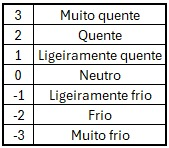
\includegraphics[width=0.3\linewidth]{Tabelas/nivel-conforto.jpeg}
    \smallcaption{Fonte: Autor. Adaptado de \textcite{mccullough1989data}.}
    \label{tab: conforto}
\end{table}

\begin{equation} \label{eq:pmv} 
    \begin{aligned}
   PMV = [0,303 \cdot e^{-0,036\cdot M}+0,028]\cdot ((M-W)-3,05\cdot10^{-3}\cdot [5733-6,99\cdot(M-W)-p_{a}]\\
   -0,42\cdot[(M-W)-58,15]-1,7\cdot 10^{-5}\cdot M \cdot(5867-p_{a})-0,0014\cdot M\cdot(34-t_{a})\\
   -3,96\cdot10^{-8}\cdot f_{cl}\cdot[(t_{cl}+273)^4-(t_{r}+273)^4]-f_{cl}\cdot h_{c}\cdot(t_{cl}-t_{a}))
    \end{aligned}
\end{equation}

A equação pode ser reescrita como a Equação \ref{eq:pmvl}. Onde $L$ é a carga térmica total do corpo.

\begin{equation} \label{eq:pmvl}
    \begin{aligned}
   PMV = [0,303 \cdot e^{-0,036\cdot M}+0,028]\cdot L
    \end{aligned}
\end{equation}

Depois de estimado o voto é possível estimar a insatisfação de conforto por meio da Equação \ref{eq:ppd}.

\begin{equation} \label{eq:ppd}
    \begin{aligned}
   PPD = 100 - 95\cdot e^{-(0,03353 PMV^4 + 0,2179PMV^2)}
    \end{aligned}
\end{equation}

Ao relacionar o \textit{PMV} com o \textit{PPD} tem-se o gráfico mostrado na Figura \ref{fig:graficopmvppd}.

\begin{figure}[!htp] 
 \centering
    \caption{Gráfico \textit{PMV} x \textit{PPD}}
    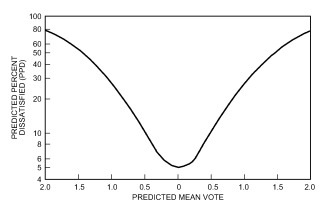
\includegraphics[width=0.6\linewidth]{Imagens/grafico-pmv-ppd.jpeg}
    \smallcaption{Fonte: \textcite{fanger1970thermal}.}
    \label{fig:graficopmvppd}
\end{figure}

\section{Normas e Parâmetros técnicos} \label{premissas}

As normas são fundamentais a fim de definir os parâmetros e condições do ambiente que propiciem não só conforto térmico às pessoas presentes em um determinado local, mas também uma boa qualidade de vida, ao passo que estas condições estão diretamente ligadas à saúde dos indivíduos.

Conforme a norma \textcite{abnt216401}, os parâmetros que influenciam na sensação de conforto térmico são: temperatura operativa, velocidade do ar e umidade relativa do ar. Assim, fatores como o tipo de roupa e nível de atividade física das pessoas podem interferir nestes parâmetros e, portanto, os intervalos de valores recomendados visam proporcionar a sensação de conforto térmico para, no mínimo, $80\%$ das pessoas.

A norma utilizada para o cálculo do conforto térmico é referente ao capítulo 9 da \textcite{ASHRAE2009} que descreve todo o processo de balanço de energia do corpo humano e conforto térmico, bem como a escala de sensação térmica, que é muito utilizada para a comparação do ambiente com a norma. 

Zonas de conforto foram determinadas pela \textit{ASHRAE} conforme a Figura \ref{fig: Zonas_Conforto}. Assim, baseando-se nestes parâmetros, a norma \textcite{abnt216401} estipula valores adequados de temperatura operativa, umidade relativa e velocidade do ar para o verão e o inverno, os quais podem ser observados na Tabela \ref{tab: Parâmetros Ar}. 

\begin{figure}[!htb] 
 \centering
    \caption{Zonas de Conforto conforme \textit{ASHRAE}}
    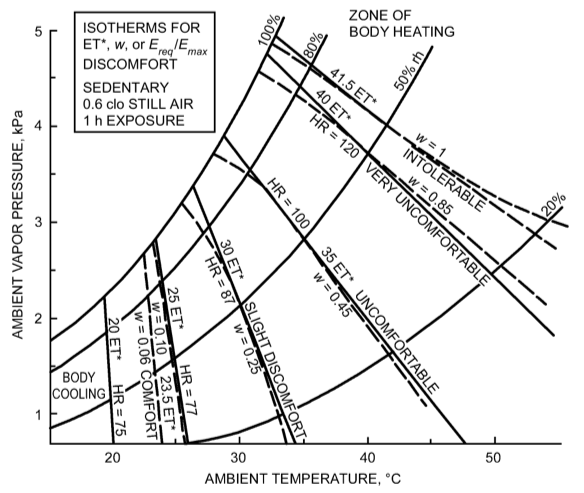
\includegraphics[width=0.8\linewidth]{Imagens/Zonas_Conforto.png}
    \smallcaption{Fonte: \textcite{ashrae2005ashrae}.}
    \label{fig: Zonas_Conforto}
\end{figure}

\begin{table}[!htb] 
 \centering
    \caption{Parâmetros adequados para o ar nas condições de verão e inverno}
    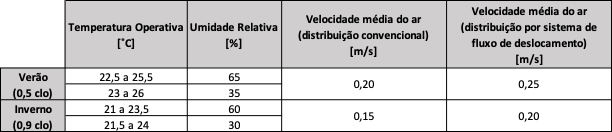
\includegraphics[width=1.0\linewidth]{Tabelas/Tabela_ABNT.png}
    \smallcaption{Fonte: Autor. Adaptado de \textcite{abnt216401}.}
    \label{tab: Parâmetros Ar}
\end{table}

Deste modo, considerando-se a pressão barométrica de São Paulo, equivalente a $92633 \space Pa$, a Figura \ref{fig:Norma_Carta_Psicrometrica} foi criada a fim de facilitar a visualização da área na qual os parâmetros estão de acordo com a norma.

\begin{figure}[!htb] 
 \centering
    \caption{Representação dos parâmetros ideais conforme norma \textcite{abnt216401} na carta psicrométrica}
    \includegraphics[width=1.0\linewidth]{Imagens/Norma_Carta_Psicrometrica.png}
    \smallcaption{Fonte: Autor.}
    \label{fig:Norma_Carta_Psicrometrica}
\end{figure}
\newpage
A região delimitada em amarelo refere-se aos parâmetros utilizados para o verão ao passo que em azul está atrelado ao inverno. Dessa maneira, vale ressaltar que a análise de um ponto na carta psicrométrica está relacionada a um conjunto de fatores, como temperatura e umidade, a fim de cruzá-lo com a região estipulada pela norma.

Outro ponto importante está ligado à quantidade de ${CO}_{2}$ que foi considerada como aceitável nesta análise, que, por ainda apresentar algumas controvérsias quanto a norma, requer uma análise um pouco mais extensa. 

O dióxido de carbono é um dos gases do efeito estufa mais encontrados na atmosfera, visto que é exalado por todo ser humano, ao passo que é possível afirmar que o dobro de pessoas gera o dobro da quantidade de ${CO}_{2}$ \cite{ashrae2001}. Geralmente, como também é o caso deste estudo, é analisado em partes por milhão (\textit{ppm}). Este gás costuma ser encontrado em valores entre os $400$ e $1000$ \textit{ppm} para áreas internas, mas pode margear os $2500$ \textit{ppm}, dadas certas situações, sendo que acaba não por ser um agente tóxico, mas sim um asfixiante simples, pois toma o lugar do oxigênio no corpo humano. Entretanto problemas reais de respiração e no sistema nervoso só ocorrem em concentrações a partir dos trinta e cinco mil \textit{ppm} \cite{handbook2017ashrae}. O mesmo artigo cita também um valor limítrofe para um dia de 8 horas de trabalho, sendo este o de $5000$ \textit{ppm}, mas é importante lembrar que no caso desta análise, onde não há fontes mais significativas de ${CO}_{2}$ além dos passageiros do Metrô, é essencialmente impossível alcançar esta marca.

De modo a estabelecer parâmetros voltados a segurança nestes ambientes internos, a Associação Brasileira de Normas Técnicas apresentou a \textcite{abnt17037}, que define um ponto saudável para a concentração de dióxido de carbono em $700$ \textit{ppm} acima da medida encontrada em área externa, substituindo portanto, a resolução n.º 9 da \textcite{anvisar9}, que afirmava um valor máximo de $1000$ \textit{ppm} independente do ar externo. A resolução antiga considerava um valor de ${CO}_{2}$ externo de $300$ \textit{ppm}, que somado aos $700$ \textit{ppm} resulta no valor apresentado, mas, visto que as taxas deste gás vêm subindo a cada ano, é necessário ajustar o máximo esperado. Estudos como o de \textcite{stoco} revelam ainda valores úteis para este estudo, já que o autor registrou aferições médias de $430,9$ $\pm$ $23,3$ \textit{ppm} do contaminante efetuadas no Instituto de Astronomia, Geofísica e Ciências Atmosféricas da USP, situado no Butantã.

Dados os apontamentos citados, é também relevante citar que recentes estudos apresentam inconsistências quanto ao efeito do dióxido de carbono sobre o comportamento humano, mas um ponto em comum é que a partir dos $1000$ \textit{ppm} há reduções na capacidade cognitiva do indivíduo \cite{astmD6245}, junto à sensação de fadiga, sonolência e até dores de cabeça, geralmente ocorrendo a partir das $2000$ \textit{ppm} \cite{silvaco2}, que ainda aumentam conforme as concentrações deste gás sobem. Este fato explica o motivo por trás dos limites recomendados pela \textcite{abnt17037} e a resolução n.º 9 da \textcite{anvisar9}, já que, apesar da mudança entre normas, o resultado é relativamente próximo ao se considerar que a concentração externa varia de $300$ a $500$ \textit{ppm} \cite{ashrae2016}. 

\section{\textit{Computational Fluid Dynamics} (\textit{CFD})}

Fluxos e fenômenos relacionados podem ser descritos a partir de equações parciais diferenciais, as quais, usualmente, não podem ser resolvidas analiticamente. Dessa maneira, o método da discretização permite aproximar tais equações a um sistema algébrico que possa ser solucionado por meios computacionais. Assim, as aproximações são aplicadas a pequenos domínios de espaço e tempo \cite{peric2002computational} para simular o fenômeno em um determinado período e, portanto, quanto menor a malha utilizada, isto é, quanto menor o domínio de espaço e tempo adotado, maior a precisão dos resultados, embora exija maior capacidade computacional. Assim, a análise numérica dos escoamentos é denominada Dinâmica dos Fluidos Computacional, que, em inglês, é representada pela sigla \textit{CFD}. 

Em estudos de conforto térmico, a dinâmica dos fluidos computacional é muito utilizada por ser uma ferramenta que consegue simular de maneira muito exata as condições térmicas do ambiente.   

Como um exemplo de estudo de conforto térmico por \textit{CFD}, é possível citar o estudo realizado por \textcite{li2019multi}. Este artigo tinha como objetivo estudar o conforto térmico dentro do carro de um trem de alta velocidade (\textit{HST}) chinês, por meio de simulações \textit{CFD} e posteriormente utilizar a krigagem (ou \textit{Kriging}, em inglês), para substituir a simulação por dinâmica dos fluidos computacional, por ser mais rápida e otimizada. Para chegar a resultados confiáveis e com o mínimo de falhas computacionais possíveis, o estudo de \textcite{li2019multi} realizou 25 simulações, no \textit{software}, com parâmetros diferentes, mas com as mesmas resoluções de malha e condições de contorno. Com os resultados das simulações, foi possível obter parâmetros como temperatura da cabine do carro, concentração de contaminantes e o \textit{PMV} (\textit{Predicted mean vote}) que é um modelo desenvolvido por \textcite{fanger1970thermal}, muito utilizado em estudos de conforto térmico, no qual se utiliza a temperatura da pele para definir o conforto.

\chapter{Materiais e Métodos}

\section{Metodologia}

O objeto deste estudo é a análise de um dos carros da frota L da linha 1 - Azul, do Metrô de São Paulo. Esta frota é uma atualização da antiga frota D, de 1986, fabricada pela MAFERSA e foi reinaugurada em 2011 como frota L através da atualização dos trens através de consórcio, sendo sua última modernização em 2017 \cite{Trens_e_frotas}. Um carro desta frota e o mapa da rede do Metrô de São Paulo são mostrados nas Figuras \ref{fig:Trem_da_Frota_L} e \ref{fig:mapa-da-rede-metro-0124-abre}.

\begin{figure}[!htb]
    \centering
    \begin{minipage}{0.45\textwidth}
        \caption{Trem da frota L do Metrô de São Paulo}
        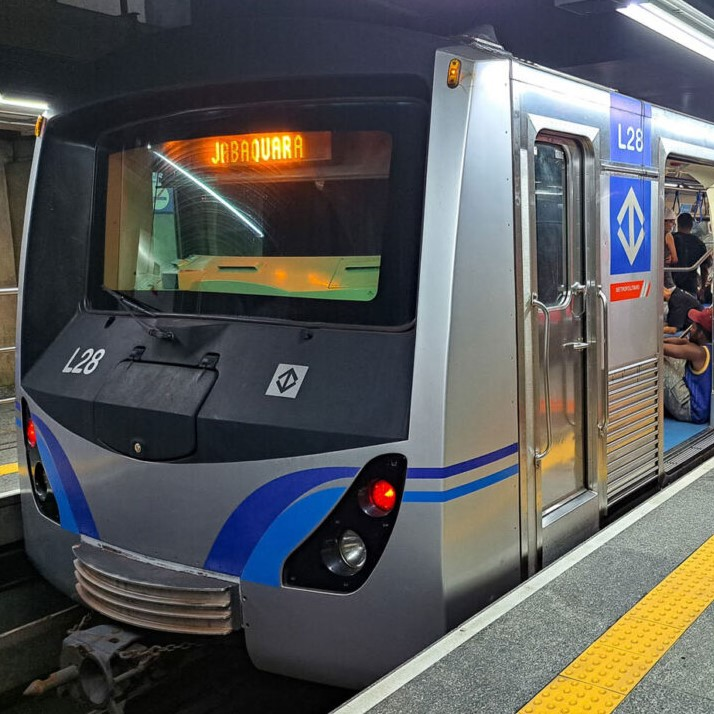
\includegraphics[width=\linewidth, height=6cm]{Imagens/Alstom_L28.jpg}
        \smallcaption{Fonte: \textcite{frotaL}.}
        \label{fig:Trem_da_Frota_L}
    \end{minipage}\hfill
    \begin{minipage}{0.45\textwidth}
        \caption{Mapa da rede de trem e Metrô da cidade de São Paulo}
        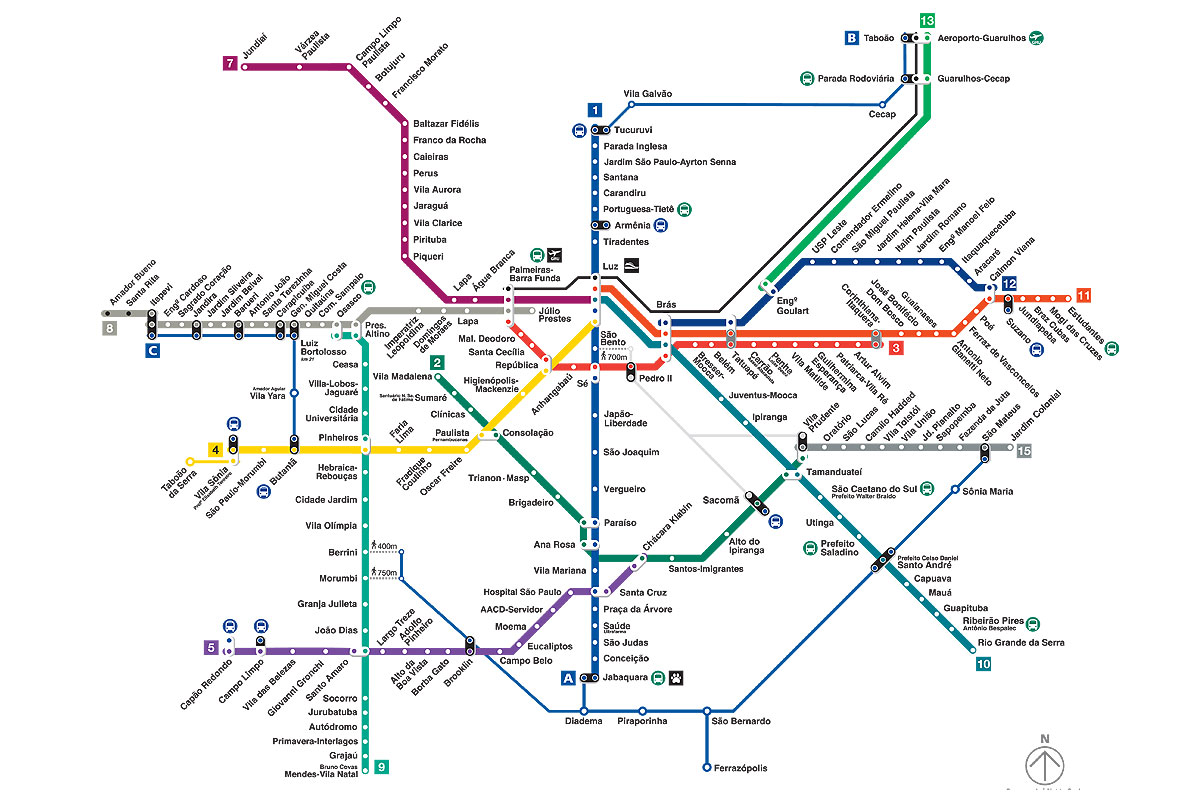
\includegraphics[width=\linewidth, height=6cm]{Imagens/mapa-da-rede-metro-0124-abre.jpg}
        \smallcaption{Fonte: \textcite{Mapametro}.}
        \label{fig:mapa-da-rede-metro-0124-abre}
    \end{minipage}
\end{figure}

Para facilitar o entendimento do trabalho, tem-se o fluxograma que resume a metodologia do estudo, esquematizado na Figura \ref{fig: Fluxograma}.

\begin{figure}[!htb] 
 \centering
    \caption{Fluxograma da metodologia}
    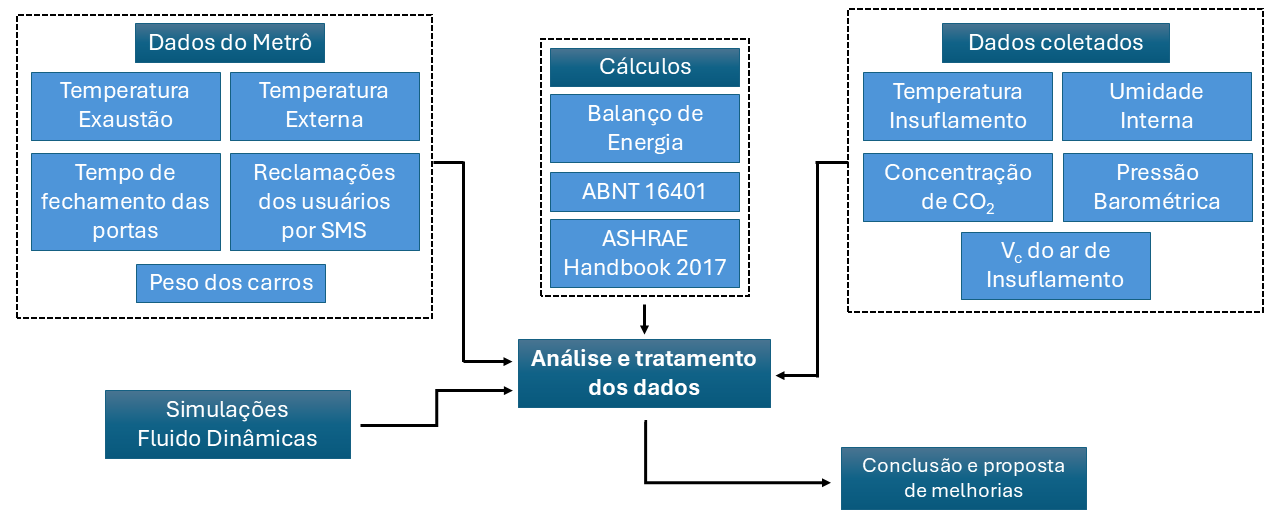
\includegraphics[width=1\linewidth]{Imagens/Fluxograma_da_metodologia.png}
    \smallcaption{Fonte: Autor.}
    \label{fig: Fluxograma}
\end{figure}
\newpage
Foi feita a pesquisa da análise dos parâmetros de conforto térmico, levando em conta as normas vigentes. Após a conclusão da pesquisa e das revisões bibliográficas, foram realizadas reuniões pontuais com a equipe do Metrô de São Paulo, nas quais as ideias do grupo foram alinhadas e discutidas com a empresa. 

A seguir, foi efetuada a escolha dos melhores sensores considerando o custo benefício e a aplicação específica empregada. Para validar o funcionamento de todos os sensores e o código desenvolvido, foram realizados testes iniciais utilizando uma \textit{protoboard}, garantido assim o funcionamento de todos os componentes em trem, e seguiu-se para próxima parte que foi o desenvolvimento de quatro \textit{Printed Circuit Boards} (\textit{PCB}), com todos os componentes já integrados. 

Foram implementadas três placas iguais com o intuito de permanecer dentro do carro do Metrô medindo os parâmetros de conforto térmico, realizando a medição das informações em três locais estratégicos. A primeira localizada na altura das pessoas na extremidade do carro, a segunda no ponto de exaustão e a última localizada no centro do carro na altura do insuflamento. Portanto, foi possível estimar uma média do local, considerando uma simetria do carro. A quarta e última placa foi utilizada para a medição da pressão do local, para que fosse possível converter os dados de umidade relativa em absoluta, e foi colocada ao lado da primeira placa de conforto térmico. É possível observar tudo o que foi descrito na Figura \ref{fig:metodo_de_medicao}. Vale ressaltar que a partir de uma conversa com o Metrô de São Paulo, foi sugerido a presença de um membro do grupo para cuidar de cada \textit{PCB}.

\begin{figure}[!htb]
 \centering
    \caption{Explicação da instalação das placas de medições}
    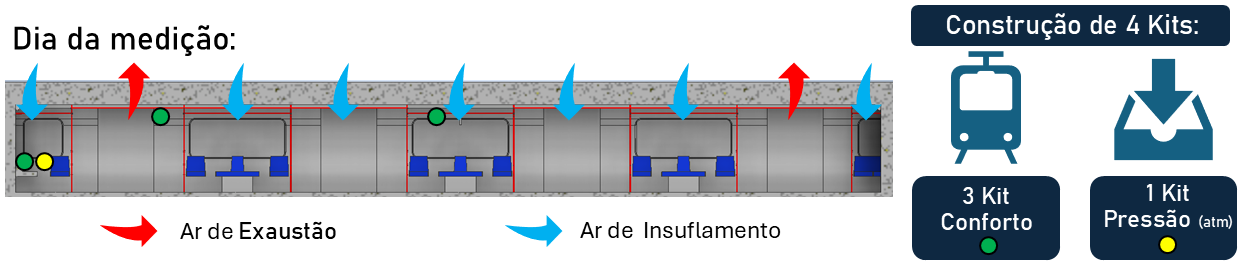
\includegraphics[width=1\linewidth]{Imagens/metodo_de_medicao.png}
    \smallcaption{Fonte: Autor.}
    \label{fig:metodo_de_medicao}
\end{figure}

Sucessivamente, com posse dos dados obtidos pelos sensores e os disponibilizados pelo Metrô de São Paulo, realizou-se o tratamento dos mesmos em um \textit{software} dedicado e elaborou-se as primeiras análises do comportamento que o ar possui no carro, e foram criadas as primeiras correlações. Simultaneamente, foram elaborados os cálculos de \textit{PMV} e \textit{PPD} e relações com as normas \textcite{abnt16655} e \textit{ASHRAE}, além de todos os cálculos termodinâmicos, assim podendo ter um comparativo com o teórico e o valor esperado pelas normas.  Posteriormente, utilizando a análise computacional, a partir do \textit{CFD}, foram gerados novos dados complementares aos instrumentais.que auxiliou para uma conclusão objetiva sobre as condições atuais do Metrô de São Paulo, além de possibilitar a elaboração de  propostas de melhorias.

\subsection{Parâmetros estabelecidos pelo Metrô de São Paulo}

O \textcite{metrosp2024} possui seus próprios parâmetros para avaliação da temperatura, pois o sistema de ar-condicionado não possui nenhum sensor de insuflamento, apenas de exaustão. Logo, para saber a temperatura esperada no ambiente, o Metrô de São Paulo definiu um parâmetro de controle de temperatura em  especificação de projeto que é definido pela Equação \ref{eq:temperaturametro}. Esta, é uma equação linear com seus termos compostos por $T_{ic}$, temperatura interna esperada, e o objetivo do sistema de ar-condicionado para o carro, $T_{adj}$, uma temperatura de ajuste, também chamada de \textit{set-point}, sendo possível alterá-la entre ${21}^\circ C$ a ${25}^\circ C$ e $T_{ext}$, que é temperatura externa. O \textcite{metrosp2024} utiliza este formato por se tratar de um método mais fluido que as normas padrões para ar-condicionado, prevenindo assim, o choque térmico dos passageiros ao entrar nos carros.

\begin{equation} \label{eq:temperaturametro}
\begin{aligned}
{T}_{ic} = {T}_{adj} + {0,25} \cdot ({T}_{ext} - {19})
\end{aligned}
\end{equation}

Estas relações de valores de temperatura são representadas em um gráfico mostrado na Figura \ref{fig:temperatura_norma_metro}, com a $T_{adj}$ variando de ${21}^\circ C$, ${23}^\circ C$ e ${25}^\circ C$. O \textcite{metrosp2024}, até o momento deste trabalho, tem $T_{adj}$ definida em  ${23}^\circ C$. A temperatura $T_{ic}$  desejada pode variar em ${2}^\circ C$ para mais ou para menos, sendo usada como parâmetro para o trabalho.

\begin{figure}[!htb]
\centering
    \caption{Relação de temperaturas para o Metrô de São Paulo}
    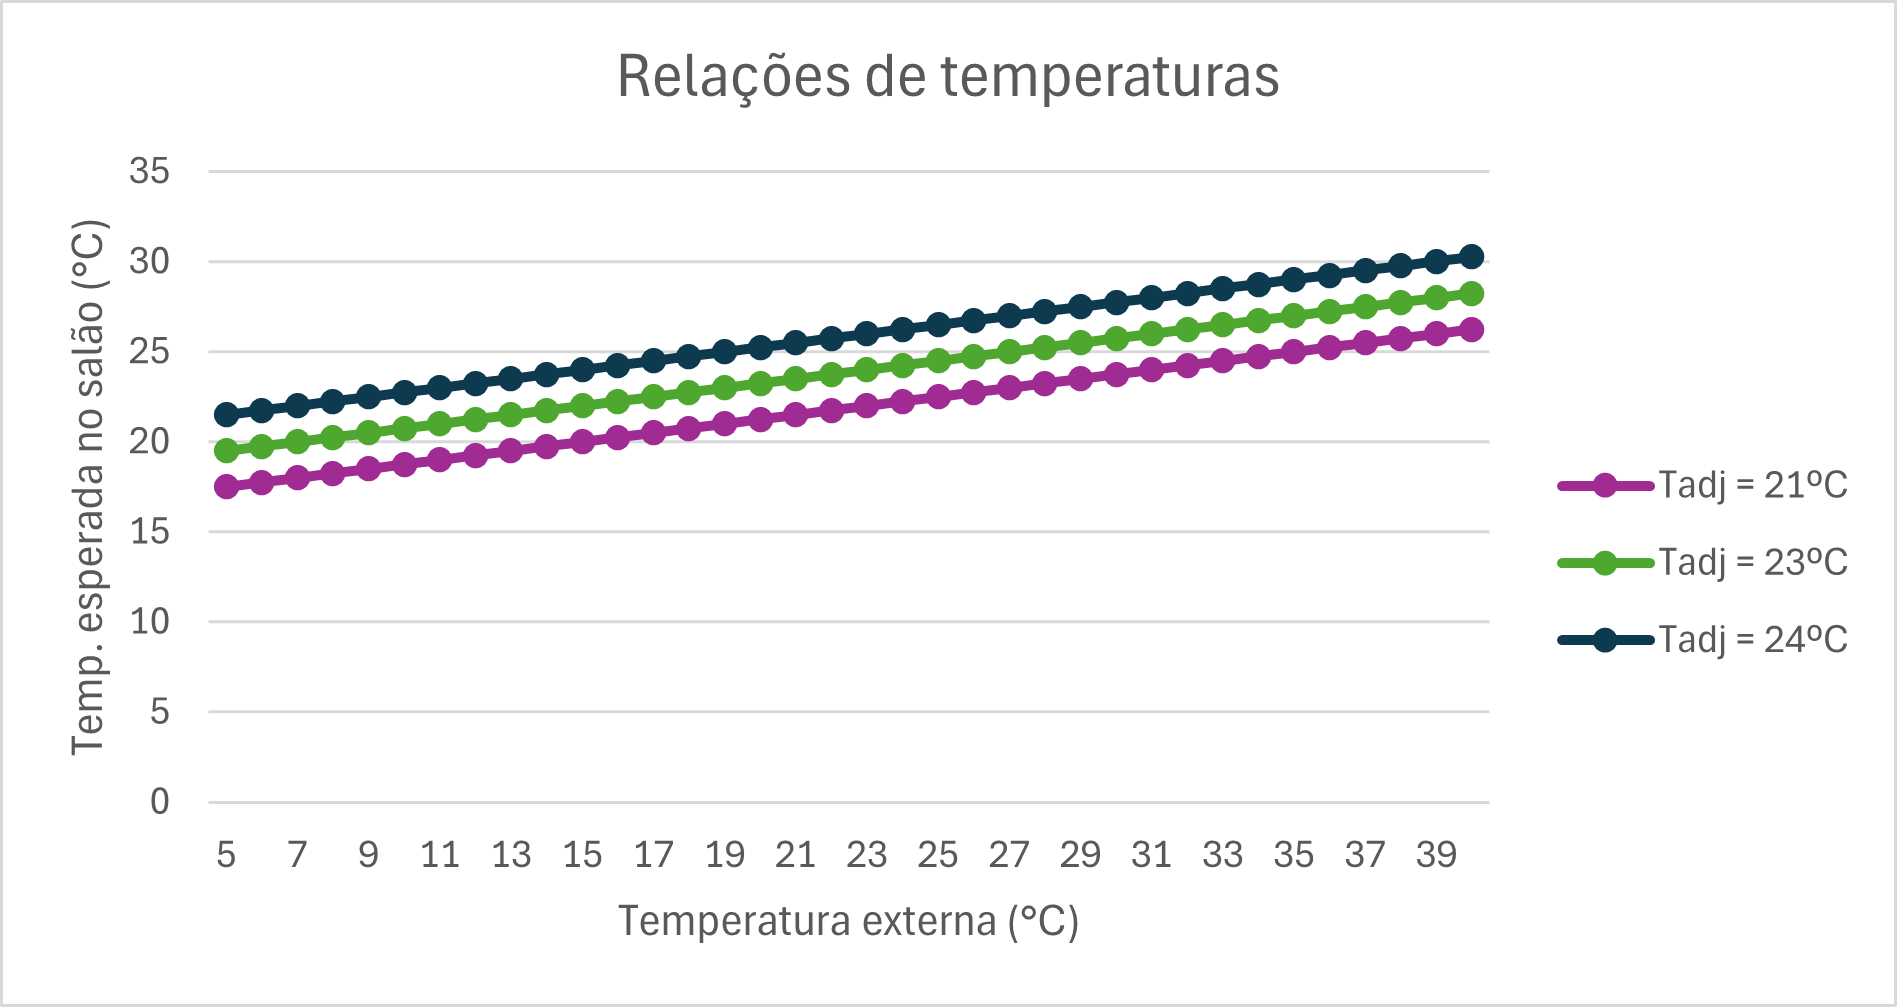
\includegraphics[width=0.8\linewidth]{Imagens/Relacoes_de_temperaturas.png}
    \smallcaption{Fonte: \textcite{metrosp2024}.}
    \label{fig:temperatura_norma_metro}
\end{figure}

Outro parâmetro importante de ser analisado é o número de pessoas no carro, que o Metrô de São Paulo também possui uma métrica própria, considerando a área total disponível de 46 $m^2$ e 48 cadeiras úteis, existem dois tipos de carregamento: um com o total de ${6}$ $passageiros/m^2$ o equivalente a 228 em pé e 48 sentadas e outro de ${8}$ $passageiros/m^2$ que equivale a 320 em pé e 48 sentadas. Para o estudo, o \textcite{metrosp2024} informou para adotar o primeiro tipo de carregamento.  

\subsection{Variáveis fixas do trabalho e simplificações} \label{simplificacao}

Para obtenção de êxito nos cálculos de conforto térmico, foram necessárias algumas simplificações visto que certos parâmetros não podem ser medidos sem um estudo mais aprofundado, o que foge do escopo deste trabalho. 

Inicialmente, as pessoas foram consideradas como sendo paralelepípedos de base quadrada com altura de $1,7$ $m$ e com $70$ $kg$ de peso, sendo uma boa estimativa para a população brasileira, para os cálculos de metabolismo e área superficial do corpo.

Em relação à situação das pessoas dentro do Metrô, foi considerado que o nível de atividade exercida dentro dos carros do Metrô foi leve ou sedentário com batimentos cardíacos menores que $90$ $bpm$ e, portanto, o consumo de oxigênio ($\dot{Q}_{O_{s}}$) foi de $8$ $mL/s$ e o $RQ$ foi constante em $0,83$. Também foram consideradas que estavam sentadas com o ar parado, ocasionando em um coeficiente de troca de calor convectivo ($h_{c}$) constante de $3,1$ $W/m^2K$ e utilizando calça e camiseta de manga curta, por isso os índices $I_{cl}$ e $f_{cl}$ foram de $0,57$ e $1,15$, respectivamente. Vale lembrar que a pressão de vapor d'água é tabelada e varia de acordo com a $t_{a}$.

A temperatura radiante média ($t_{r}$) foi considerada igual à temperatura ambiente ($t_{a}$), porque para medi-la seriam necessárias medidas mais específicas. Também foi considerado para efeito de contas, que a temperatura do salão do Metrô (temperatura ambiente) é igual à temperatura de exaustão, mas somente para o modelo.
   
Considerou-se que o carro não possui entradas de ar externo por meio de frestas e, portanto, a carga térmica desta fonte foi desprezada. Além disso, para facilitar a análise da carga térmica, objetivou-se a variação da energia equivalente a zero ao longo do tempo a fim de manter um regime permanente. Por fim, a região das janelas foi considerada com a mesma composição das paredes ou portas, uma vez que, embora o vidro possua uma espessura menor, sua área também é reduzida quando comparado à parede e, portanto, através de cálculos, foi possível concluir que o fluxo de calor não possui grandes variações entre os dois casos.

Sobre a questão dos parâmetros de dióxido de carbono (${CO}_{2}$), foi também realizada uma simplificação para a posterior análise de seus níveis no carro. Idealmente, deveriam ser realizadas medições dos níveis de ${CO}_{2}$ externos ao carro em conjunto com o sensoriamento interno. Entretanto, após diálogos com a equipe do Metrô, revelou-se que um kit externo ocasionaria alguns problemas, dada as limitações dos possíveis locais de fixação do mesmo. Assim, tomando como base os apontamentos da seção \ref{premissas}, ao se adicionar os níveis externos do gás, que variam de $300$ a $500$ partes por milhão, aos $700$ \textit{ppm} recomendados pela \textcite{abnt17037}, são evidenciados valores de $1000$ a $1200$ \textit{ppm} como os limites ideais. 

Entretanto, deve-se levar em consideração as características do sistema de ar por onde passa a linha azul. Apesar de, em sua maioria, serem presentes as estações e tuneis subterrâneos, há também uma grande quantidade de momentos onde o Metrô passa por áreas abertas, além de que a ventilação observada nos pontos subterrâneos funciona de maneira muito eficiente, renovando constantemente o ar que passa por lá. Além disso, outra base vem do valor evidenciado por \textcite{stoco}, oriundo de uma área externa em local denso da cidade de São Paulo, que também pode ser adaptado para este projeto.

Levando em conta as informações supracitadas, o ambiente exterior ao carro, que é majoritariamente interno, foi considerado como tendo as propriedades de uma área externa, e com isso foi selecionada, para este estudo, uma concentração de $500$ \textit{ppm} de ${CO}_{2}$, que é o limite superior que se pode considerar para esta classificação. Com estes fatos e a norma em mente, o limite saudável da concentração de dióxido de carbono estabelecido para esta análise fica situado em $1200$ \textit{ppm}.

De modo a reunir as informações expostas nesta e na seção \ref{premissas}, pode se apresentar à Tabela \ref{tab:tabelaco2}, produzida pelo grupo com base nos estudos expostos pela \textcite{abnt17037}, \textcite{handbook2017ashrae}, \textcite{astmD6245}, \textcite{silvaco2} e \textcite{ashrae2016}, sendo útil para se obter algumas referências frente a análise exposta na seção \ref{comparagrupo}.

\begin{table}[!htb] 
 \centering
    \caption{Níveis de concentração de ${CO}_{2}$ e seus respectivos efeitos nos passageiros}
    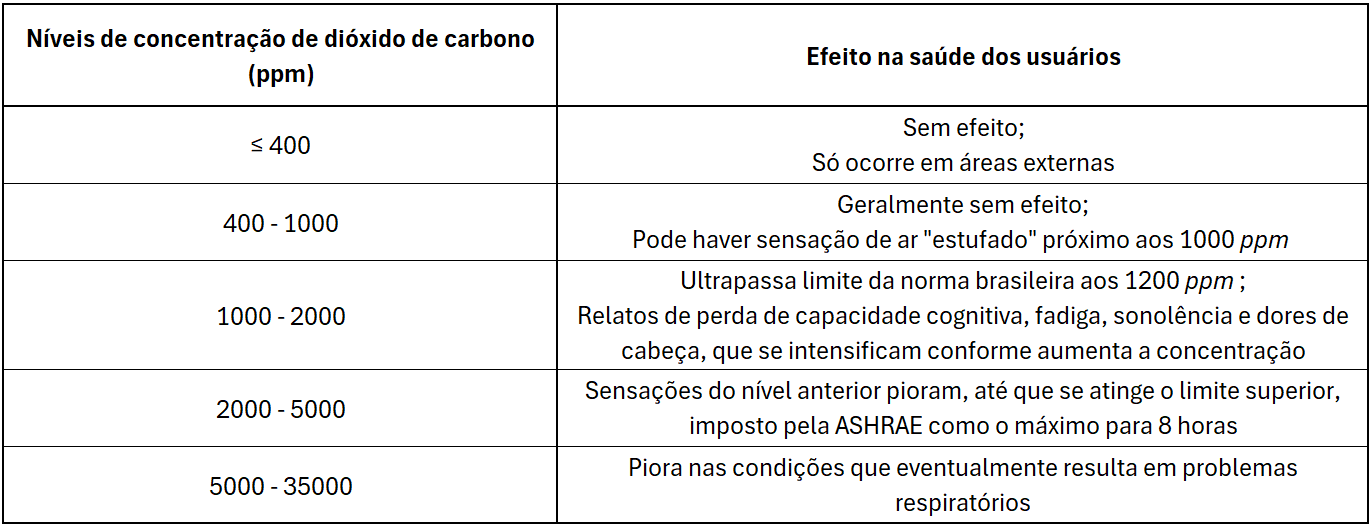
\includegraphics[width=0.8\linewidth]{Tabelas/tabela_co2.png}
    \smallcaption{Fonte: Autor. Adaptado de \textcite{abnt17037}, \textcite{handbook2017ashrae}, \textcite{astmD6245}, \textcite{silvaco2} e \textcite{ashrae2016}.}
    \label{tab:tabelaco2}
\end{table}

\section{Sistema de aquisição de dados}

A aquisição de dados é parte fundamental do trabalho, sendo a base para futuras análises e correlações. Como descrito na seção \ref{confortotermico}, certos parâmetros como temperatura, umidade e a qualidade do ar interferem diretamente na percepção do que é agradável ou não para as pessoas. Logo é necessária uma robustez dos dados que foram coletados e aferidos.

Parte dos dados apresentam caráter quantitativo, como a temperatura do ar de insuflamento e de exaustão. Outros dados se apresentam em caráter mais qualitativo, como a opinião das pessoas sobre a temperatura em um determinado estado de tempo. Parte do trabalho, portanto, é analisar a correlação desses dados.

Além da divisão dos tipos de dados, há a divisão da fonte dos mesmos, sendo que uma parte foi obtida diretamente pelo Metrô de São Paulo, como:

\begin{itemize}
    \item Reclamação dos passageiros via \textit{SMS};
    \item Peso do carro ao longo do tempo;
    \item Temperatura externa;
    \item Temperatura de exaustão.
\end{itemize}    

E uma segunda parte dos dados foi obtida a partir da instrumentação adicional do carro:

\begin{itemize}
    \item Temperatura de insuflamento;
    \item Temperatura de exaustão;
    \item Temperatura interna média;   
    \item Velocidade do ar de insuflamento;
    \item Umidade interna; 
    \item Pressão Barométrica;
    \item Concentração de $CO_2$. 
\end{itemize}    

Deste modo, é possível definir os quatro kits que foram montados para as medições das condições dos carros. Foram dispostos um em uma das extremidades, outro próximo às portas, e o último mais no meio do carro, como já mencionado. Cada kit foi composto por um microcontrolador acoplado a \textit{PCB} com sensores de temperatura, umidade e concentração de $CO_2$, denominados de Kit Conforto e um último kit, cuja localização foi compartilhada com um dos outros, composto também por um microcontrolador acoplado à \textit{PCB} mas somente com sensor de pressão barométrica, chamado de Kit Pressão.

\subsection{Sensores} \label{sensor}

De modo a obter êxito na conclusão dos objetivos gerais e específicos deste trabalho, é necessária a utilização de alguns sensores propícios à obtenção dos dados quantitativos previamente citados. %Um sensor nada mais é do que um equipamento que, em contato com o ambiente que se deseja analisar, transforma variações físicas em um sinal elétrico correspondente, que deve ser posteriormente recebido, interpretado e armazenado, com o auxílio de um controlador. 
Assim, estes sensores devem ser capazes de funcionar no local de estudo, por tempo suficiente para a obtenção das informações necessárias. É válido citar também que a possibilidade de usar alguns sensores já instalados no carro, como o de temperatura, peso e indicador de abertura de portas, foi plenamente explorada, de modo a nutrir as análises.

Para a medição de velocidade foi utilizado o TESTO 405 - Anemômetro e Termômetro compacto, Figura \ref{fig:TESTO_405}, que opera tanto como termômetro medindo temperatura, como anemômetro medindo a velocidade do ar. Para as medições de temperatura opera de ${-20} ^{\circ}C$ até ${50}^{\circ}C$ com uma acurácia de ${0,5}^{\circ}C$. Para as velocidade opera de ${0}$ a ${10}$ ${m/s}$ para intervalo de temperatura de ${0}$ até ${50} ^{\circ}C$, com uma acurácia de $\pm {0,3}$ ${m/s}$ $+{5}\%$ da velocidade medida e resolução de ${0,01}$ ${m/s}$ que é mais que o suficiente para o trabalho \cite{TESTO_405}.

\begin{figure}[!htb]
\centering
    \caption{TESTO 405 - Anemômetro e Termômetro compacto}
    \includegraphics[width=0.15\linewidth]{Imagens/TESTO_405.png}
    \smallcaption{Fonte: \textcite{TESTO_405}.}
    \label{fig:TESTO_405}
\end{figure}


O sensor de temperatura que foi utilizado, DS18B20, opera de $3,0$ a $5,5$ \textit{Volts} e foi escolhido devido a sua boa reputação em aplicações ligadas a \textit{VAC} e facilidade de montagem, ao funcionar com protocolo \textit{One-Wire}, onde, além da pinagem necessária para energização, \textit{GND} e \textit{VDD},  padrão para todos os componentes, transmite seus dados aquisitados por apenas uma via, denominada \textit{DQ}, havendo tanto envio quanto recebimento de sinal por meio de uma porta digital.  O \textit{layout} desta pinagem é apresentado na Figura \ref{fig:PinTemp}, onde são vistos, além dos pinos citados, as letras "NC", que dizem respeito às conexões não utilizadas.

\begin{figure}[!htb]
\centering
    \caption{Diagrama da pinagem do sensor DS18B20}
    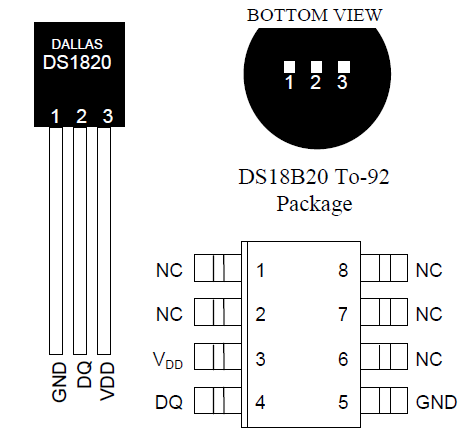
\includegraphics[width=0.30\linewidth]{Imagens/PinTemp.png}
    \smallcaption{Fonte: \textcite{DS18B20}.}
    \label{fig:PinTemp}
\end{figure}

\newpage

Outras vantagens deste sensor incluem sua capacidade de funcionamento sem outros componentes, o que elimina a necessidade de uma placa de interpretação, além de um intervalo de medição de temperatura satisfatório ao projeto, variando entre ${-55}^{\circ}C$ a ${+125}^{\circ}C$, com uma resolução padrão de $0,5^{\circ}C$, configurável até $0,0625^{\circ}C$ a partir de uma alteração do número de \textit{bits} utilizado para leitura \cite{DS18B20}.

De acordo com seu \textit{datasheet}, de onde foram extraídos os dados supramencionados, este equipamento opera, de maneira simplificada, com base em uma variação de tensão produzida conforme alteração da temperatura, que por sua vez é convertida como um sinal digital e armazenada na memória interna do dispositivo, composta por $16$ \textit{bits} e denominada de \textit{scratchpad}. Este valor é enviado ao controlador, que recebe e armazena os dados coletados. O diagrama de blocos referente ao sensor pode ser visto na Figura \ref{fig:DiagBlocTemp}. 

\begin{figure}[!htb]
\centering
    \caption{Diagrama de blocos para o sensor DS18B20}
    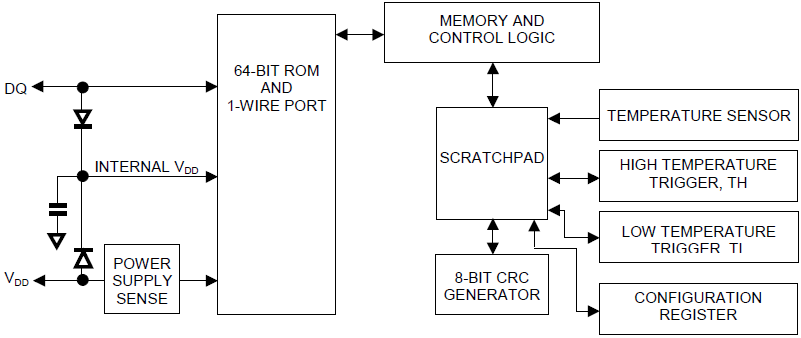
\includegraphics[width=0.8\linewidth]{Imagens/DiagBlocTemp.png}
    \smallcaption{Fonte: \textcite{DS18B20}.}
    \label{fig:DiagBlocTemp}
\end{figure}

Além das vantagens já mencionadas, outro benefício deste equipamento diz respeito à sua função de alarme, que funciona a partir dos gatilhos presentes "\textit{HIGH TEMPERATURE TRIGGER, TH}" e "\textit{LOW TEMPERATURE TRIGGER, TL}", vistos também na Figura \ref{fig:DiagBlocTemp}, para altas e baixas temperaturas, respectivamente. Contanto que a função tenha sido especificada no código, um conjunto de sensores DS18B20 em paralelo pode perceber uma variação acima dos limites definidos pelo usuário e acusar qual sensor recebeu esta informação, indicando, por exemplo, uma discrepância maior de temperatura na região próxima à abertura das portas do carro. Existem diversas bibliotecas para o uso desse sensor, como a \textit{Arduino Temperature Control Library} de \textcite{Arduino-Temperature-Control-Library}.

A respeito do sensor de umidade selecionado, HDC1080, seu \textit{datasheet}, revela que opera em um intervalo de tensão elétrica similar ao de temperatura, de $2,7$ a $5,5$ \textit{Volts}, além de possuir uma precisão satisfatória quanto a obtenção de valores de umidade relativa, variando em apenas $2\%$, validando a coleta de dados. Outras vantagens incluem o baixo consumo energético e o pequeno tamanho, o que facilita a montagem no espaço a ser utilizado \cite{HDC1080}. A pinagem necessária pode ser vista na Figura \ref{fig:PinHum}, onde \textit{SDA} representa a linha serial de dados, que deve ser conectada ao controlador, transmitindo em velocidade padrão de $11$ \textit{bits} por segundo, \textit{SCL} representa o relógio serial, que mantém o conjunto controlador/sensor em sincronia, e \textit{GND}, \textit{VDD}, e "NC" cumprem as mesmas funções previamente citadas.

\begin{figure}[!htb]
\centering
    \caption{Diagrama da pinagem do sensor HDC1080}
    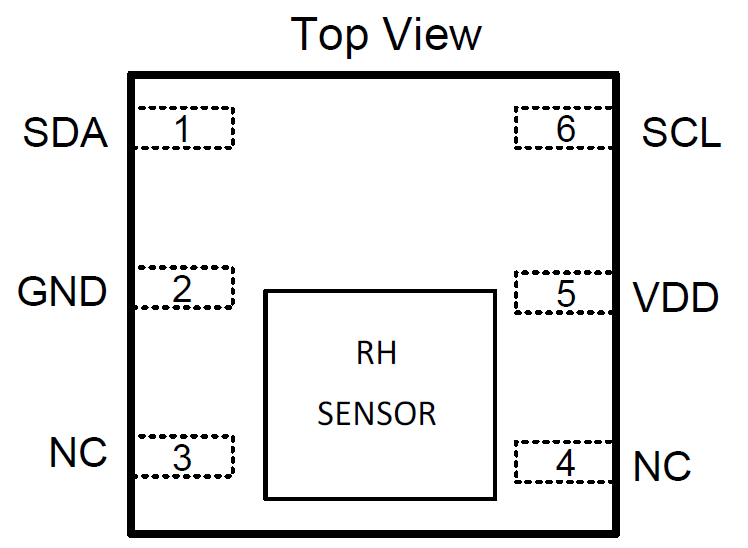
\includegraphics[width=0.4\linewidth]{Imagens/PinHum.png}
    \smallcaption{Fonte: \textcite{HDC1080}.}
    \label{fig:PinHum}
\end{figure}

Existem outros motivos que levaram a escolha deste sensor, dentre eles a ótima reputação de seu fabricante, \textit{Texas Instruments}, que sugere dentro do próprio \textit{datasheet} a aplicação em sistemas de \textit{VAC}, condizendo com o caso estudado, e também a presença de um sensor secundário de temperatura. Este sensor foi de grande auxílio às análises, pois apresentou um caráter de validação ao trabalhar em conjunto com os sensores de temperatura já utilizados, tanto do Metrô, quanto o escolhido. A partir de um conjunto de sensores com a mesma função, é possível confirmar que os dados colhidos condizem com a realidade, descobrir padrões, ou ainda encontrar um aparelho defeituoso, por exemplo. 

Assim, é de interesse do grupo utilizar este sensor suplementar, que opera de modo muito similar ao sensor de temperatura previamente mencionado, em conjunto com a leitura da umidade, que ocorre com a reação entre a camada de poliamida do sensor e a umidade do ar, traduzida para um valor de resistência, e pode por sua vez ser interpretada como um sinal digital no controlador. Um diagrama de blocos que representa a operação pode ser visto na Figura \ref{fig:DiagBlocHum}, onde "MCU" representa o controlador.

\begin{figure}[!htb]
\centering
    \caption{Diagrama de blocos para o sensor HDC1080}
    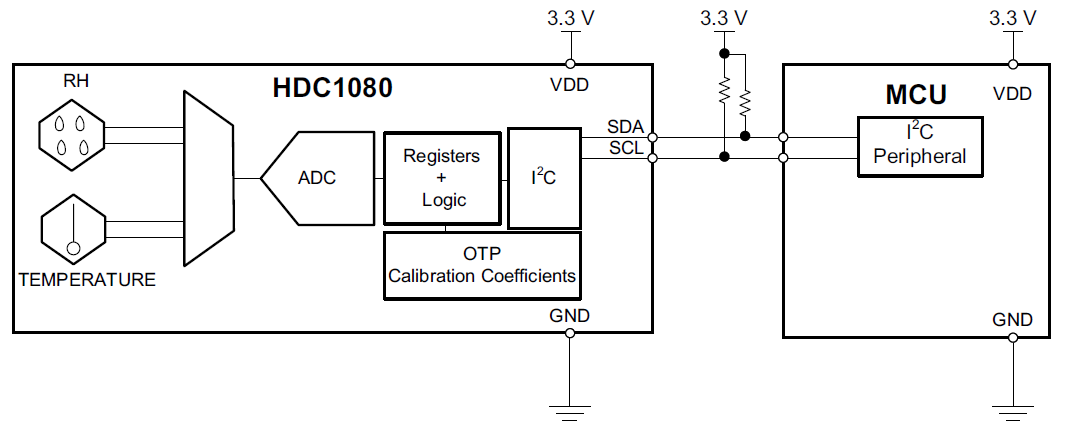
\includegraphics[width=0.75\linewidth]{Imagens/DiagBlocHum.png}
    \smallcaption{Fonte: \textcite{HDC1080}.}
    \label{fig:DiagBlocHum}
\end{figure}

Outras vantagens deste sensor incluem a funcionalidade \textit{HEAT}, que aquece o sensor de modo a reduzir a condensação que pode se acumular no próprio, derivada especialmente de uma operação próxima a um sistema de ar condicionado, além de seu próprio modo de funcionamento, que se divide em um modo de operação, onde o sensor aquisita e envia seus dados, e um modo dormente, onde permanece aguardando uma nova coleta e consumindo quantidades negligenciáveis de energia. A biblioteca existente para esse sensor é a \textit{ClosedCube} HDC1080 \textit{Arduino} do \textcite{ClosedCubeHDC1080}.

Sobre o sensor de ${CO}_{2}$, o modelo escolhido foi o SCD30, produzido pela \textit{SENSIRION}. De acordo com seu \textit{datasheet}, sua tensão elétrica de operação varia de $3,3$ a $5,5$ \textit{Volts}, sendo capaz de realizar medições dentro do intervalo de $400$ a $10000$ \textit{partes por milhão} para uma variação de apenas $30$ $ppm$ \cite{SCD30}. Este modelo já vem calibrado de fábrica, entretanto o fabricante revela que, para resultados mais precisos, é ideal mantê-lo energizado por aproximadamente uma semana em ambiente externo, que geralmente apresenta baixo índice de dióxido de carbono. O consumo de corrente médio é de $19$ $mA$, chegando a um máximo de $75$ $mA$ durante as medições, além de operar em temperaturas de $0$ a $50$ $^{\circ}C$, o que é satisfatório para o projeto. 

Um diagrama indicando a pinagem do sensor pode ser visto na Figura \ref{fig:PinCO2}, onde \textit{VDD} e \textit{GND} cumprem as mesmas funções já mencionadas, \textit{TX/SCL} faz a transferência de dados do sensor para o controlador, além do relógio serial, \textit{RX/SDA} recebe informações vindas do controlador, como um pedido de início de medição, por exemplo, \textit{RDY} indica que os dados estão prontos para coleta, \textit{PWM} envia um valor de tensão elétrica variável que indica a concentração de ${CO}_{2}$ e \textit{SEL} seleciona as diferentes interfaces do sensor.

\begin{figure}[!htb]
\centering
    \caption{Diagrama da pinagem do sensor SCD30}
    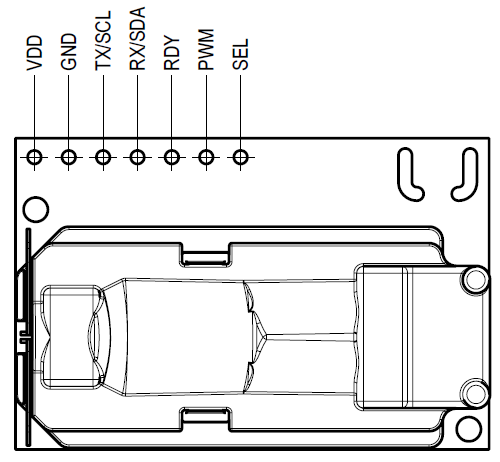
\includegraphics[width=0.5\linewidth]{Imagens/PinCO2.png}
    \smallcaption{Fonte: \textcite{SCD30}.}
    \label{fig:PinCO2}
\end{figure}

Este dispositivo utiliza a tecnologia \textit{NDIR}, ou \textit{Nondispersive infrared}, para realizar a leitura dos níveis de ${CO}_{2}$ no ambiente. De maneira simplificada, o sensor utiliza um pequeno diodo emissor de luz infravermelha instalado dentro de um tubo que se comunica com o ambiente via uma entrada e saída.  Neste invólucro, há também um sensor óptico baseado nas características de uma molécula de ${CO}_{2}$,  de modo que quando o ar dentro deste tubo é bombardeado com a luz mencionada, há uma absorção dos raios por parte das moléculas do gás analisado, fazendo com que o sensor óptico, ao realizar a leitura, obtenha uma concentração menor do que a prévia, para um caso de aumento da substância estudada, por exemplo \cite{NDIR}. Esta diferença é, então, contabilizada pelo sensor que, por sua vez, envia os dados para o controlador e assim a medição é concluída.

É válido citar que, de modo similar ao sensor de umidade escolhido, este sensor de ${CO}_{2}$ também possui equipamentos redundantes ao projeto, como um sensor de temperatura e um de umidade relativa, ambos com características satisfatórias ao necessário para a análise. Como já foi citado, estes sensores auxiliares validam as coletas realizadas, garantindo uma maior credibilidade ao estudo. Além disso, a presença deste sensor dispensa a necessidade de outro para aquisição de ${O}_{2}$, visto que este parâmetro pode ser estimado a partir dos resultados obtidos. A biblioteca existente para esse sensor é a \textit{Adafruit} SCD30 da \textcite{Adafruit_SCD30}. 

Por fim, a respeito do último sensor selecionado, pode-se citar o BMP280, produzido pela \textit{BOSCH}, como o sensor de pressão barométrica escolhido para o projeto. Este sensor realiza a medição da pressão atmosférica absoluta em um intervalo de $300$ a $1100$ $hPa$, equivalente a aproximadamente $+9000$ (acima) e $-500$ (abaixo) metros do nível do mar, com uma precisão de $\pm$ $0,12$ $hPa$, equivalente a $\pm$ $1$ $metro$. O sensor realiza estas medições para uma tensão elétrica de $1,7$ a $3,3$ \textit{Volts}, consumindo uma corrente muito baixa, de $2,7$ $\mu$$A$, além de operar dentro de um intervalo de temperatura de $-40$ a $85$ $^{\circ}C$, condições propícias ao projeto. Entre outras vantagens, seu pequeno tamanho se destaca, visto que foi desenvolvido para aplicações \textit{mobile}, ou seja, para dispositivos móveis, facilitando o posicionamento em sua respectiva placa.

A escolha deste sensor foi facilitada, considerando as especificações já mencionadas e a reputação de seu fabricante, que possui anos de experiência nesta e em outras áreas de aplicação. Assim, descrevendo as conexões realizadas com o controlador, tem se a Figura \ref{fig:PinPress}, onde \textit{VCC} e \textit{GND} realizam as mesmas funções já citadas, mas para uma conexão de $3,3$ \textit{Volts}, \textit{SCL} representa a entrada do relógio serial, \textit{SDA} representa a entrada de dados vindos do controlador, \textit{CSB} representa o seletor de interfaces, já que o sensor pode operar com diferentes controladores (neste caso, deve ser conectado a uma tensão secundária), e \textit{SDO} realiza o envio dos dados coletados pelo sensor para o controlador. É válido citar que, enquanto estas informações foram extraídas do \textit{datasheet}, produzido pela \textcite{BMP280}, este não é o caso da Figura \ref{fig:PinPress}, pois o documento mencionado apresenta diretamente as conexões feitas ao microchip, isto é, diretamente ao sensor, que necessita de uma placa secundária para interface com o controlador selecionado devido ao seu pequeno tamanho.

\begin{figure}[!htb]
\centering
    \caption{Definição de pinos do BMP280}
    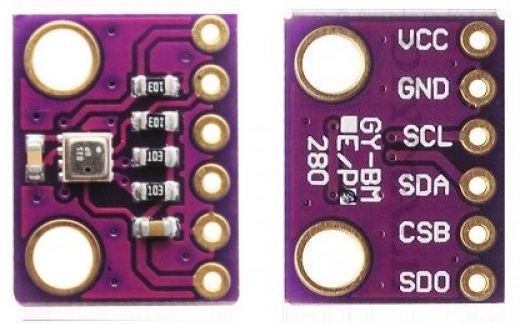
\includegraphics[width=0.25\linewidth]{Imagens/PinPress.png}
    \smallcaption{Fonte: \textcite{imgBMP280}.}
    \label{fig:PinPress}
\end{figure}

A respeito de seu princípio de funcionamento, denominado de piezo resistivo, o mesmo ocorre com a deformação de um diafragma interno por efeito de uma pressão aplicada, geralmente construído de silicone e calibrado com base na pressão a ser medida, neste caso a atmosférica, que é mensurada por um \textit{strain gauge}, ou seja, um extensômetro, o que causa uma alteração na resistência percebida na ponte de \textit{Wheatstone} presente dentro do componente. De maneira análoga, conforme a resistência é alterada, a tensão que passa pelo sensor também sofre uma alteração, o que pode ser enviado para o controlador e interpretado como a pressão atmosférica do ambiente presente \cite{piezo}, sendo um exemplo disto visto na Figura \ref{fig:piezoresist}.

\begin{figure}[!htb]
\centering
    \caption{Princípio de funcionamento de um sensor piezo resistivo}
    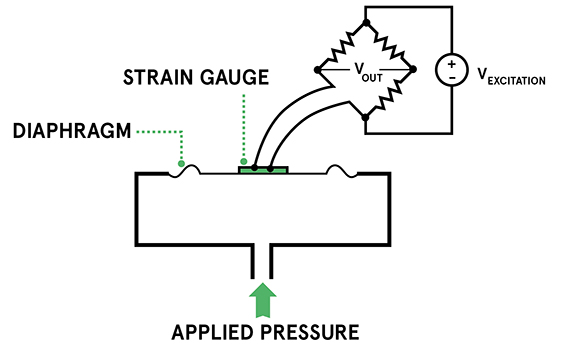
\includegraphics[width=0.4\linewidth]{Imagens/piezoresist.jpg}
    \smallcaption{Fonte: \textcite{imgpiezo}.}
    \label{fig:piezoresist}
\end{figure}

A partir da medição de pressão barométrica, este sensor permite, portanto, o cálculo da altitude em que se encontra, informação relevante para a obtenção da situação climática, por exemplo. Outro ponto extremamente importante, visto até como o principal motivo para a escolha de um sensor de pressão, é a necessidade deste valor para que a umidade relativa, obtida com os outros sensores, possa ser convertida corretamente para umidade absoluta, fator mais explorado nas seções \ref{balenergia} e \ref{ventilação}. Além disso, como outra vantagem, este equipamento também possui um sensor de temperatura redundante ao projeto, que foi usado com o mesmo propósito de validação de dados. A biblioteca existente para esse sensor é a \textit{Adafruit} BMP280 da \textcite{Adafruit_BMP280}. 

Definidos todos os sensores que auxiliam o grupo a obter os dados desejados para a análise, pode se resumir esta seção por meio da apresentação da Figura \ref{fig:fluxosenso}, onde é evidenciado um fluxograma com o parâmetro medido e o sensor utilizado junto a um resumo do que foi feito neste projeto. Junto ao mesmo, há também fotos ilustrativas dos sensores.

\begin{figure}[!htb]
\centering
    \caption{Fluxograma dos sensores}
    \includegraphics[width=1\linewidth]{Imagens/Fluxograma_dos_sensores.png}
    \smallcaption{Fonte: Autor.}
    \label{fig:fluxosenso}
\end{figure}
\newpage
\subsection{Protoboard} \label {Proto}

A partir das escolhas dos sensores na seção \ref{sensor}, conseguiu-se fazer a seleção do microcontrolador. Segundo \textcite{kerschbaumer2013microcontroladores}, os microcontroladores são circuitos integrados que possuem em seu interior todos os componentes necessários para seu funcionamento, dependendo unicamente da fonte de alimentação externa. Logo, eles agem como o cérebro de toda a parte eletrônica responsável pelo fluxo de dados e pela computação dos mesmos.

A placa de prototipagem escolhida foi o \textit{Arduino Nano}, Figura \ref{fig:pinagem arduino}, integrada pelo microcontrolador \textit{ATmega328} \cite{UNO}. A principal vantagem da escolha da plataforma \textit{Arduino}, além do seu custo relativamente acessível, é a facilidade para desenvolver software com ela. A linguagem para desenvolver códigos é uma versão simplificada de \textit{C} e \textit{C++}, e para contribuir ainda mais, existem na casa de milhões de bibliotecas online, que são programas criados por outros usuários de modo a facilitar a interface com diferentes componentes, como os sensores que foram utilizados neste projeto, podendo ser usadas gratuitamente dado a natureza do ecossistema \textit{Arduino}, facilitando assim boa parte do desenvolvimento do algorítimo base. Os sensores escolhidos já possuem bibliotecas preestabelecidas que foram utilizadas pelo grupo.

\begin{figure}[!htb]
\centering
    \caption{Pinagem do Arduino Nano}
    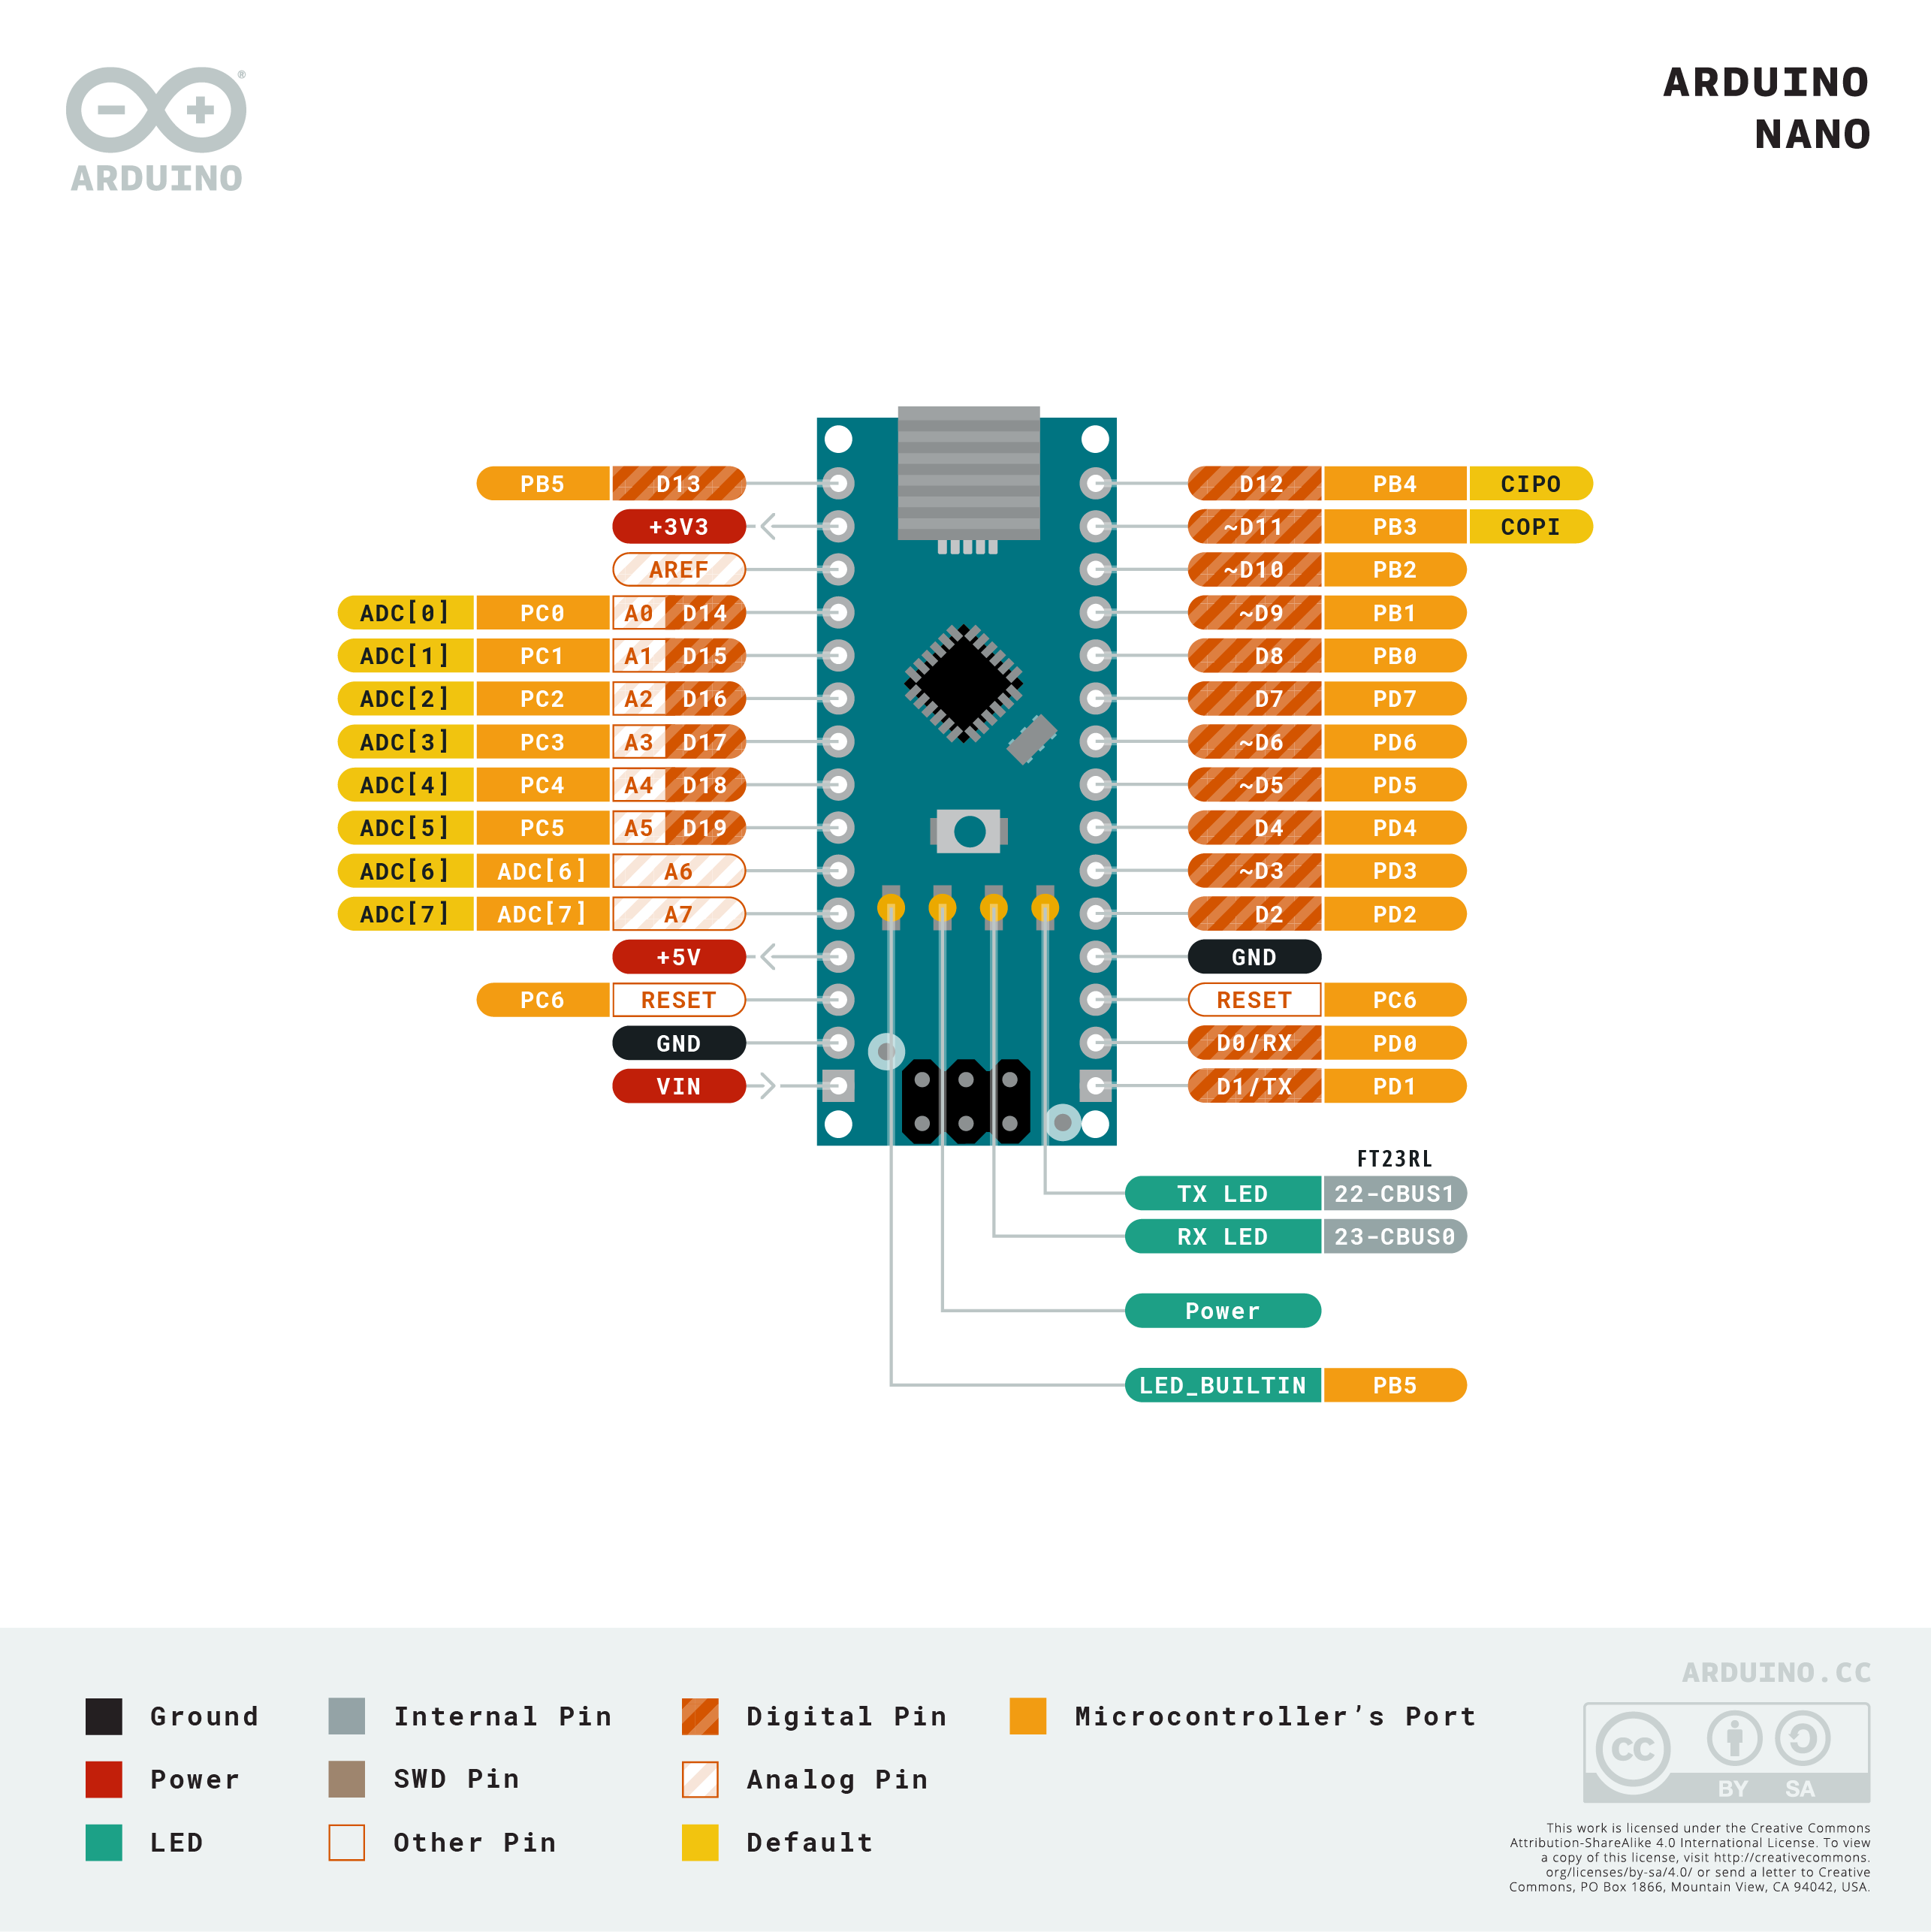
\includegraphics[width=0.85\linewidth]{Imagens/Pinagem_Arduino_Nano.png}
    \smallcaption{Fonte: \textcite{UNO}.}
    \label{fig:pinagem arduino}
\end{figure}

Para armazenamento de dados foi utilizado o \textit{Módulo Micro SD Card}, Figura \ref{fig:FotomicroSD}, que é um adaptador que transfere os dados gerados pelos sensores e interpretados pelo \textit{Arduino} para um cartão \textit{Micro SD} externo removível, pois o \textit{Arduino Nano} possui $32$ $kB$ \textit{flash} de memória \cite{UNO}, com o papel de armazenar o programa feito para ler os sensores e os dados gerados pelos mesmos. Com a utilização do \textit{Módulo Micro SD Card} é possível transferir todos os dados gerados em um cartão \textit{Micro SD} que pode ser de $2$ $GB$ até $2$ $TB$ de memória, resolvendo o problema de armazenamento e conseguindo registrar o máximo de dados que os sensores puderem fornecer. A vantagem de usar um cartão \textit{Micro SD} para o armazenamento é que já existem bibliotecas acessíveis para seu uso, como a desenvolvida pelo próprio \textit{Arduino}, denominada apenas de \textit{SD}, e encontrada pré-instalada no \textit{Arduino IDE}, como apresentado por \textcite{ArdMicroSD}. Para a análise de seu funcionamento, foi adicionado um \textit{LED} ao Arduino que varia conforme a leitura ocorre. Caso o cartão SD não seja reconhecido, o \textit{LED} permanece aceso, até que apague após resolução do problema. Entretanto, no caso de ser reconhecido, mas o arquivo não está sendo gravado corretamente, o mesmo pisca e, novamente, apaga após o funcionamento retornar ao normal.

\begin{figure}[!htb]
\centering
    \caption{\textit{Módulo Micro SD Card}}
    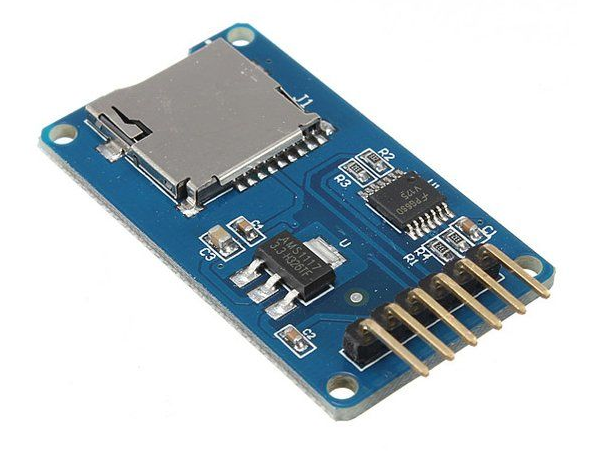
\includegraphics[width=0.3\linewidth]{Imagens/microsd.png}
    \smallcaption{Fonte: \textcite{prototype}.}
    \label{fig:FotomicroSD}
\end{figure}

Com a seleção do microcontrolador e do sistema de armazenamento, é possível seguir para o esquemático e montagem das \textit{protoboards}, que são as placas de teste que permitem a montagem de circuitos eletrônicos temporários, com a função de testar o funcionamento dos componentes e o código desenvolvido.

Usando como base todos os \textit{datasheets} dos componentes e o uso do \textit{software} \textit{KiCAD}, foi possível fazer os primeiros esquemáticos, Figuras \ref{fig:footprintprotoboardint} e \ref{fig:footprintpressao}, que apresentam todos os componentes e conectores escolhidos, alimentados por uma fonte regulada de $5$ $V$, que é a tensão em que o \textit{Arduino Nano} e uma parte dos componentes operam. Assim, tanto para o Kit Conforto quanto para o Kit Pressão, a ideia do grupo consiste em utilizar bancos de baterias portáteis, popularmente conhecidos como \textit{Power Banks}, que possibilitam alimentar as placas corretamente com 5 \textit{Volts}.

\begin{figure}[!htb]
\centering
    \caption{\textit{Footprint} para montar a \textit{protoboard} - Kit Conforto}
    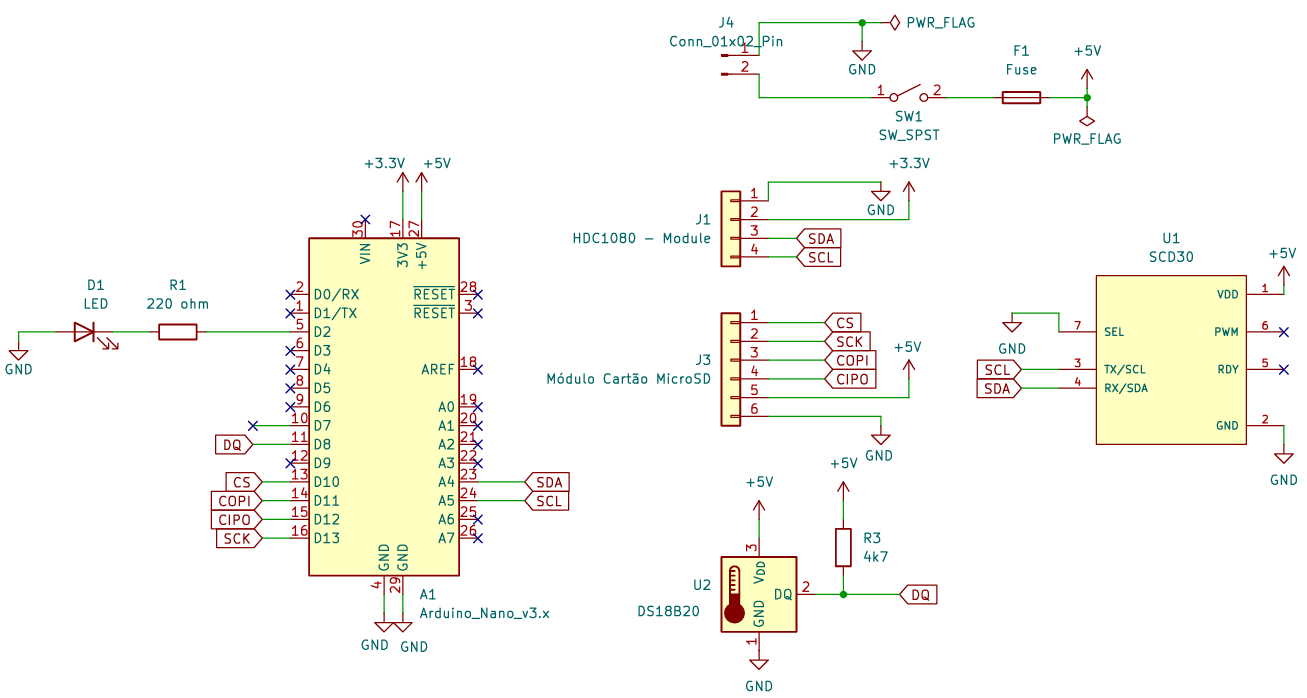
\includegraphics[width=0.7\linewidth]{Imagens/footprintprotoboardint.png}
    \smallcaption{Fonte: Autor.}
    \label{fig:footprintprotoboardint}
\end{figure}

\begin{figure}[!htb] 
\centering
    \caption{\textit{Footprint} para montar a \textit{protoboard} - Kit Pressão}
    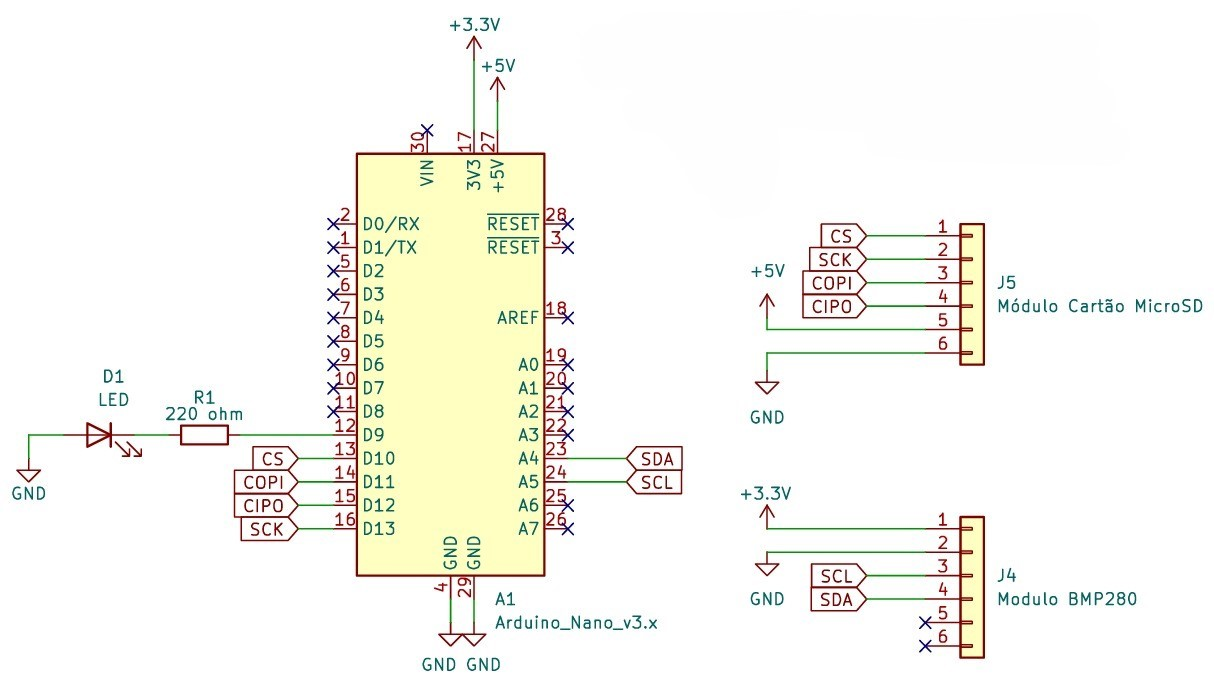
\includegraphics[width=0.7\linewidth]{Imagens/footprintpressao.jpg} 
    \smallcaption{Fonte: Autor.}
    \label{fig:footprintpressao}
\end{figure}
\newpage
De modo a comprovar e validar os \textit{footprints}, pode se apresentar as \textit{protoboards} nas Figuras \ref{fig:protoconforto} e \ref{fig:protopressao}, que representam a montagem do kit em um estágio anterior às \textit{PCBs}, pois possuem o exato comportamento esperado do produto final, mas em um formato facilmente alterável, caso ocorram problemas. Assim, é possível testar tanto o código quanto os componentes adquiridos, garantindo que tudo funcione para os dias de coleta de dados.

\begin{figure}[!htb]
\centering
    \caption{\textit{Protoboard} montada - Kit Conforto}
    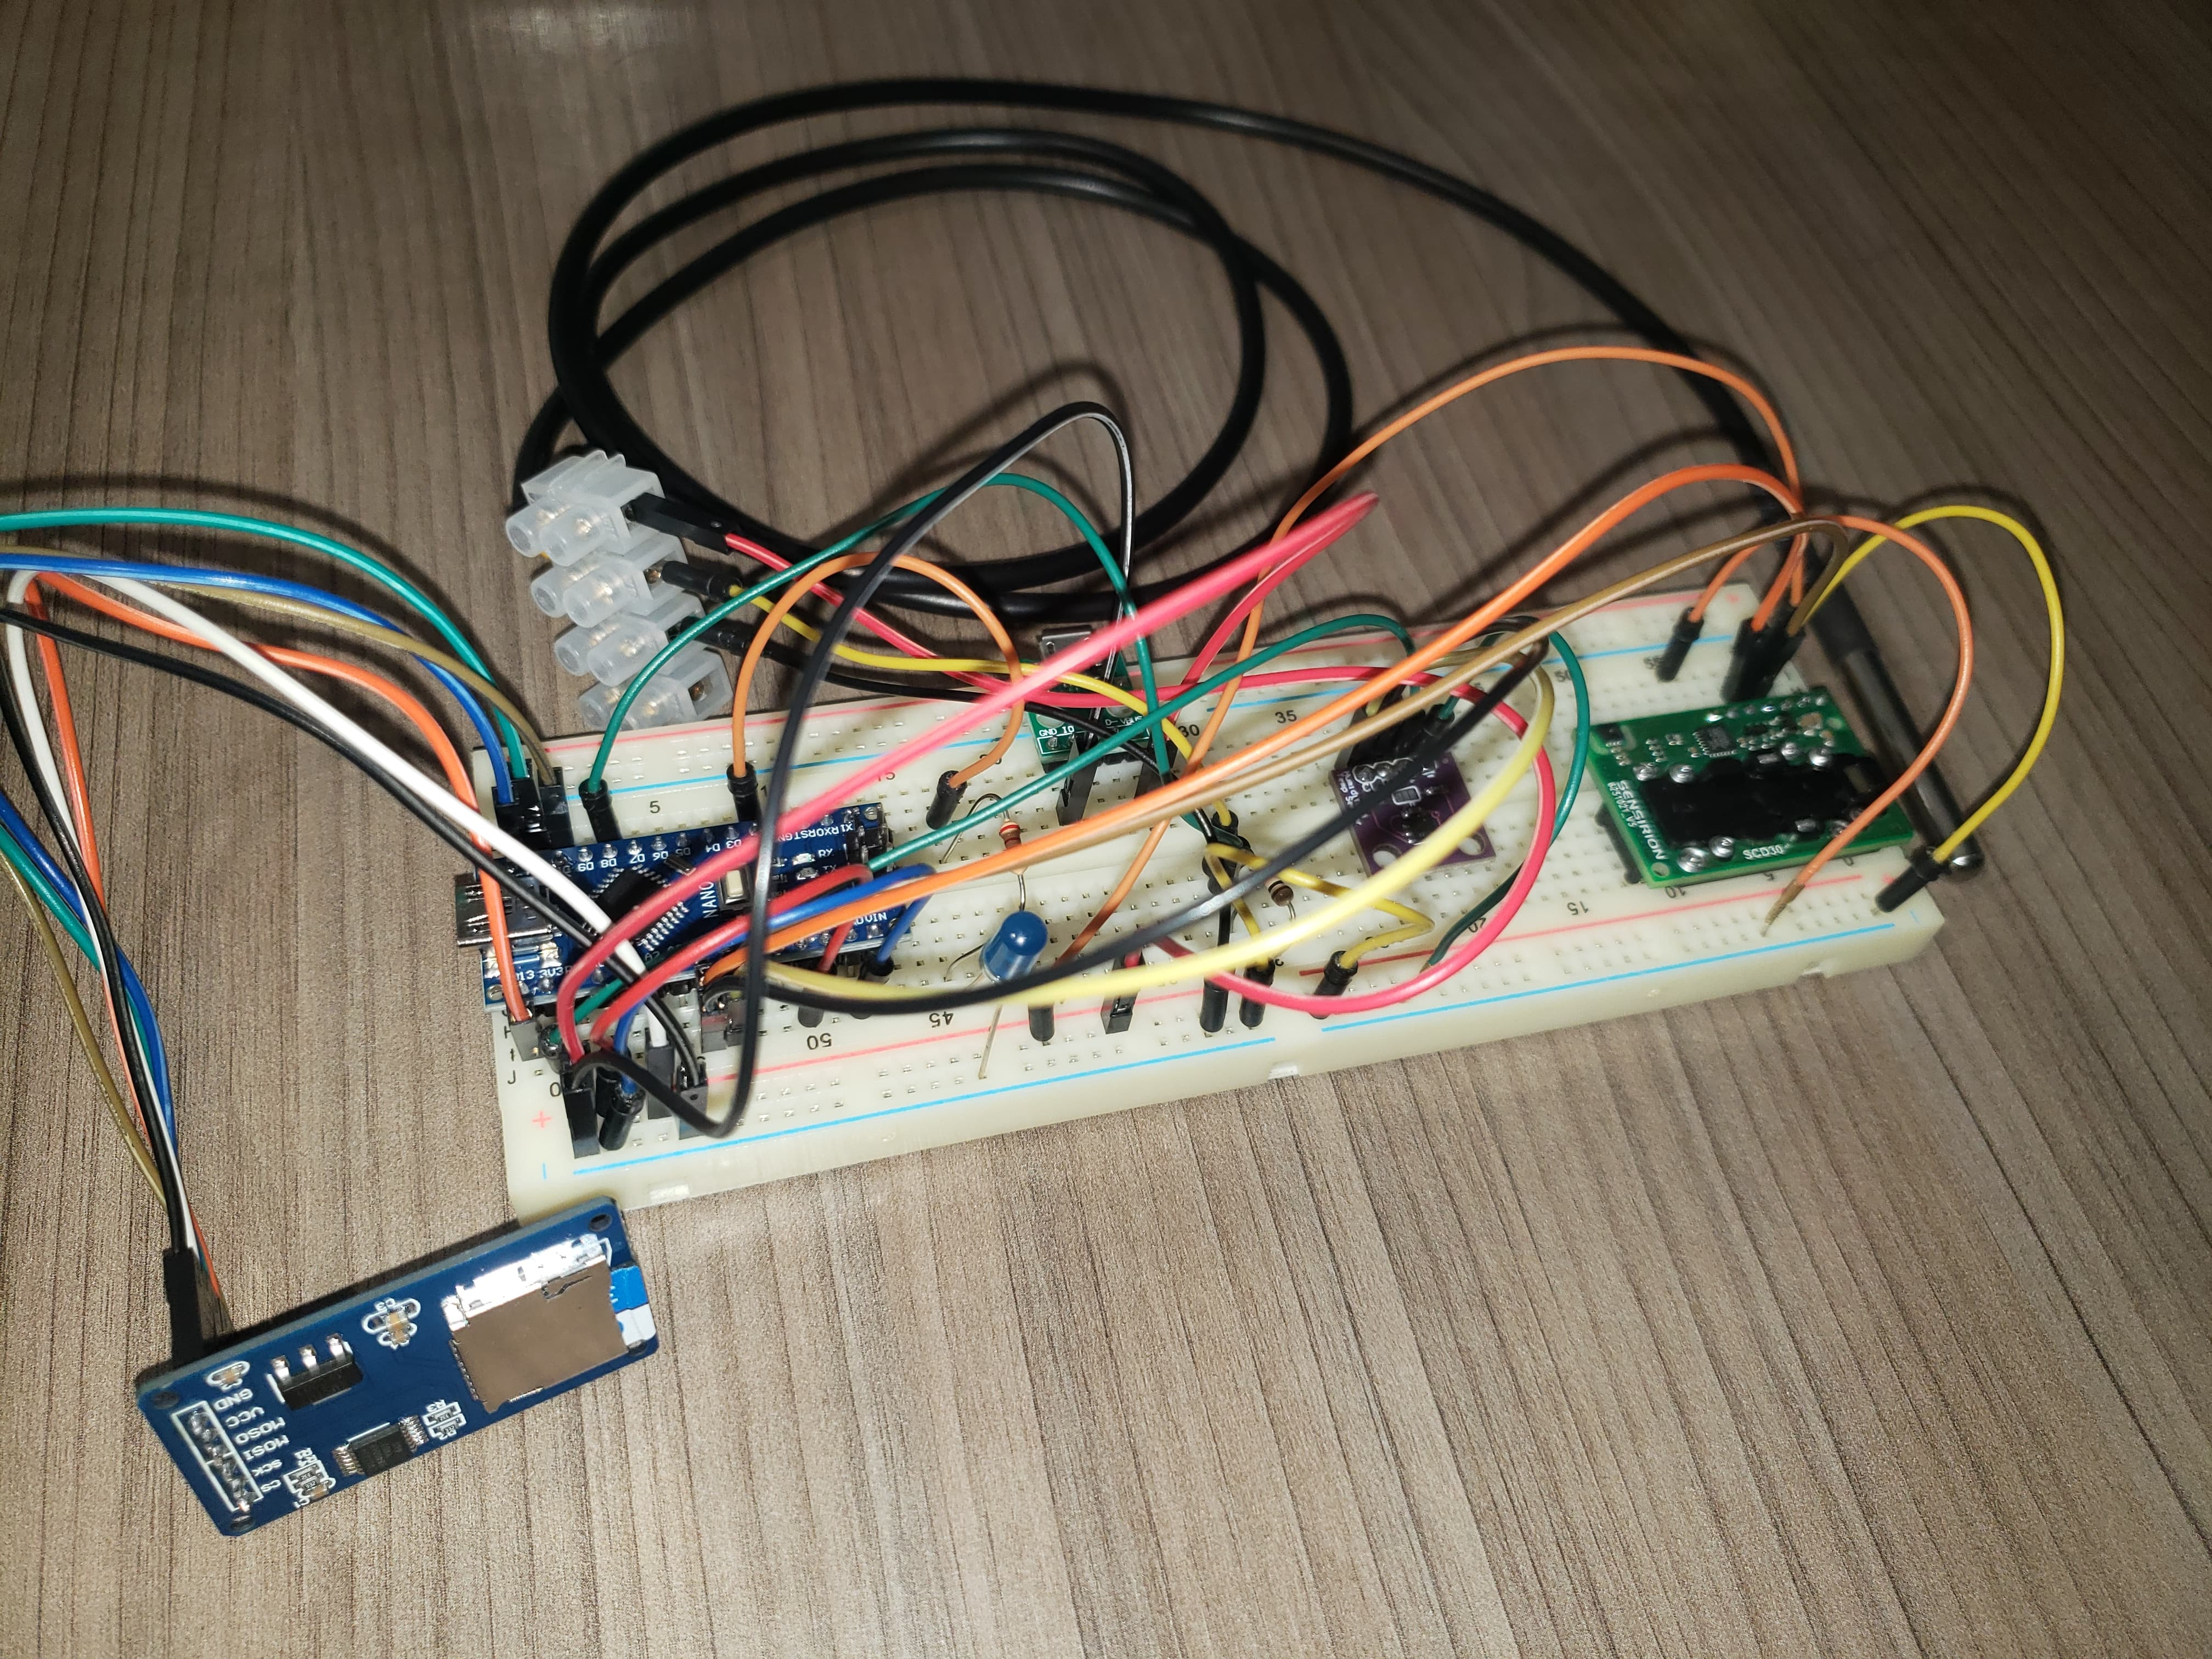
\includegraphics[width=0.65\linewidth]{Imagens/protoboardmovel.jpeg}
    \smallcaption{Fonte: Autor.}
    \label{fig:protoconforto}
\end{figure}

\begin{figure}[!htb]
\centering
    \caption{\textit{Protoboard} montada - Kit Pressão}
    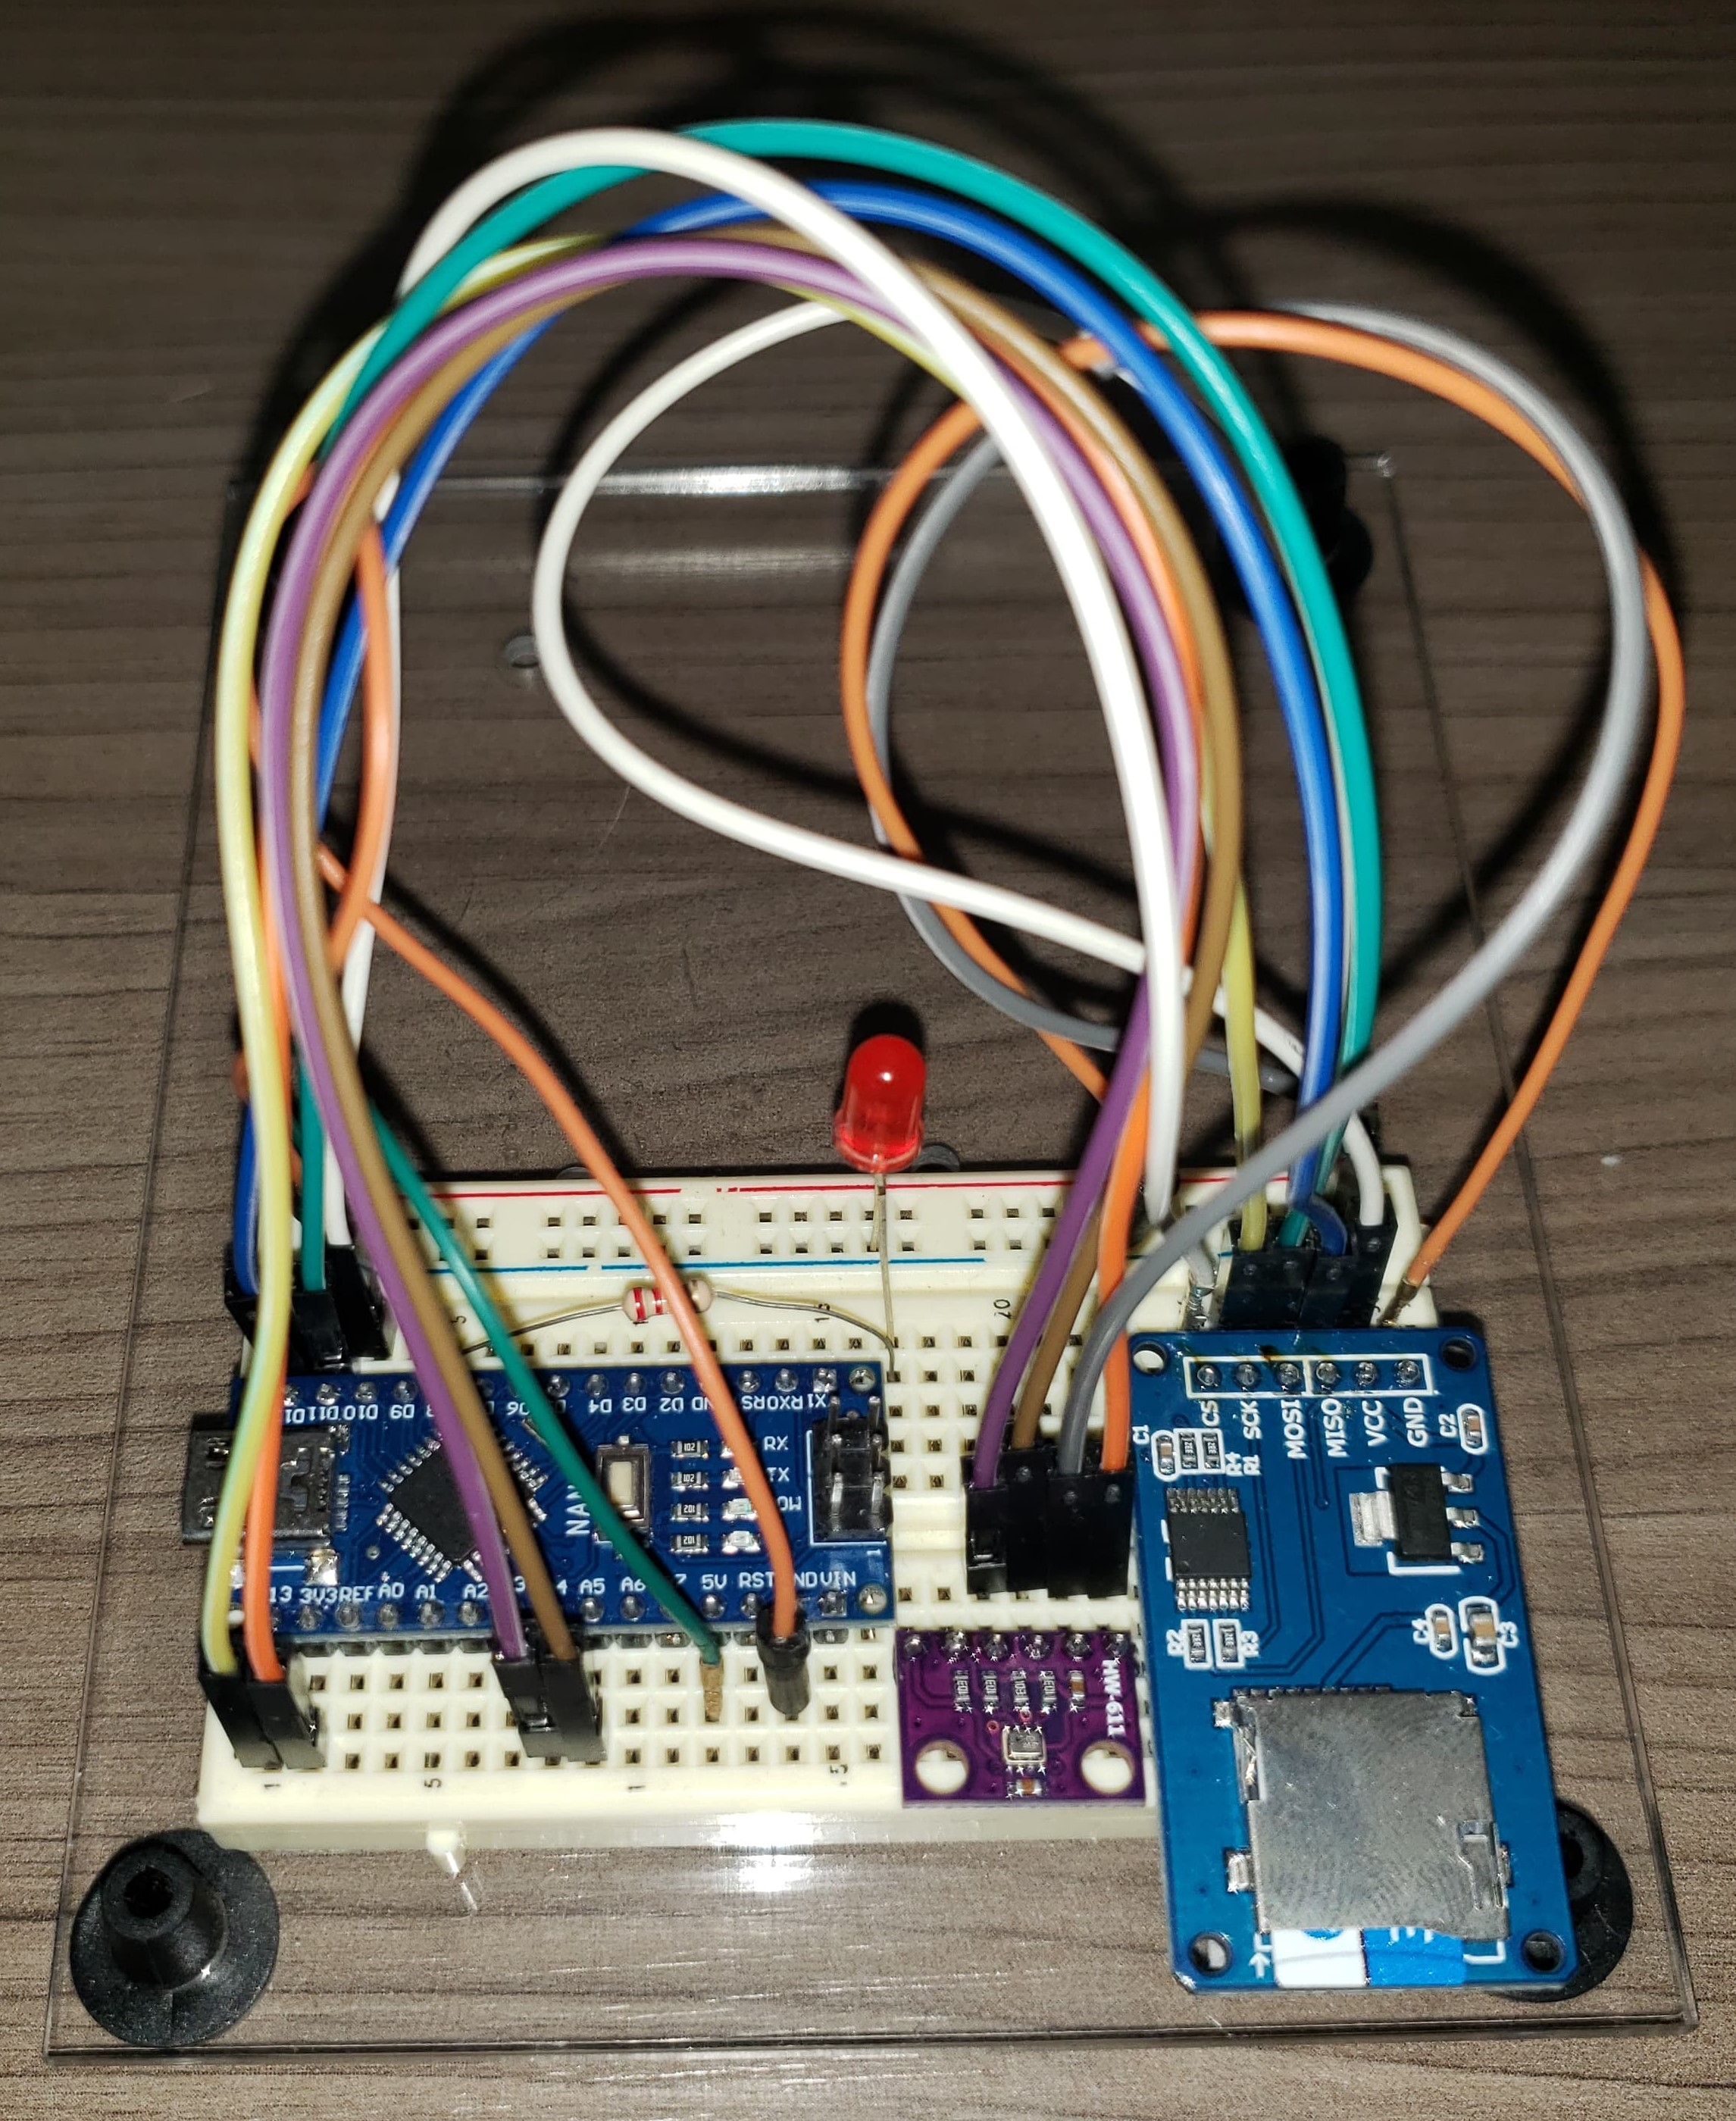
\includegraphics[width=0.45\linewidth]{Imagens/protoboardpressao.jpeg}
    \smallcaption{Fonte: Autor.}
    \label{fig:protopressao}
\end{figure}
\newpage
Uma vez montadas as \textit{protoboards}, já com o código que as acompanha bem definido, houve uma fase de testes que durou pouco mais de uma semana. Este tempo foi gasto de modo a, como dito anteriormente nesta seção, validar o funcionamento de todo o conjunto, mas também para realizar a calibração correta dos sensores, como é especificado pelos fabricantes nos \textit{datasheets} de cada sensor utilizado. O sensor de ${CO}_{2}$, por exemplo, requer um período de sete dias energizado em um local aberto, para que possa estabelecer um padrão e entender o que é um ambiente com baixos níveis de gás carbônico, o que em troca resulta numa instrumentação mais precisa. Além disso, o grupo também buscou entender melhor a questão da alimentação das placas, realizando testes também da utilização dos \textit{Power Banks}, onde o conjunto permaneceu ligado durante tempo suficiente para validar seu funcionamento, sendo esta questão melhor detalhada na seção \ref{PCB} a seguir.


\subsection{\textit{Printed Circuit Board (PCB)}} \label{PCB}

A \textit{Printed Circuit Board (PCB)} é o modelo final após a validação com a \textit{protoboard}, onde os componentes geralmente estão soldados à placa, o que garante não só uma estética melhor ao projeto, mas, fator de maior importância, um funcionamento com menor propensão a falhas, pois os componentes estão corretamente fixados à placa. Entretanto, deve-se considerar que este estágio é final, dificultando alterações no sistema, especialmente em campo, pois nesse momento não é comum possuir as ferramentas corretas para isso. Pensando nisso, o grupo optou pela utilização de barras de pinos do tipo macho e fêmea, expostas nas Figuras \ref{fig:barramacho} e \ref{fig:barrafemea}, respectivamente, onde as barras de tipo macho foram soldadas aos componentes, e as de tipo fêmea, às \textit{PCBs}.

\begin{figure}[!htb]
    \centering
    \begin{minipage}{0.45\textwidth}
        \caption{Barra de pinos de tipo macho}
        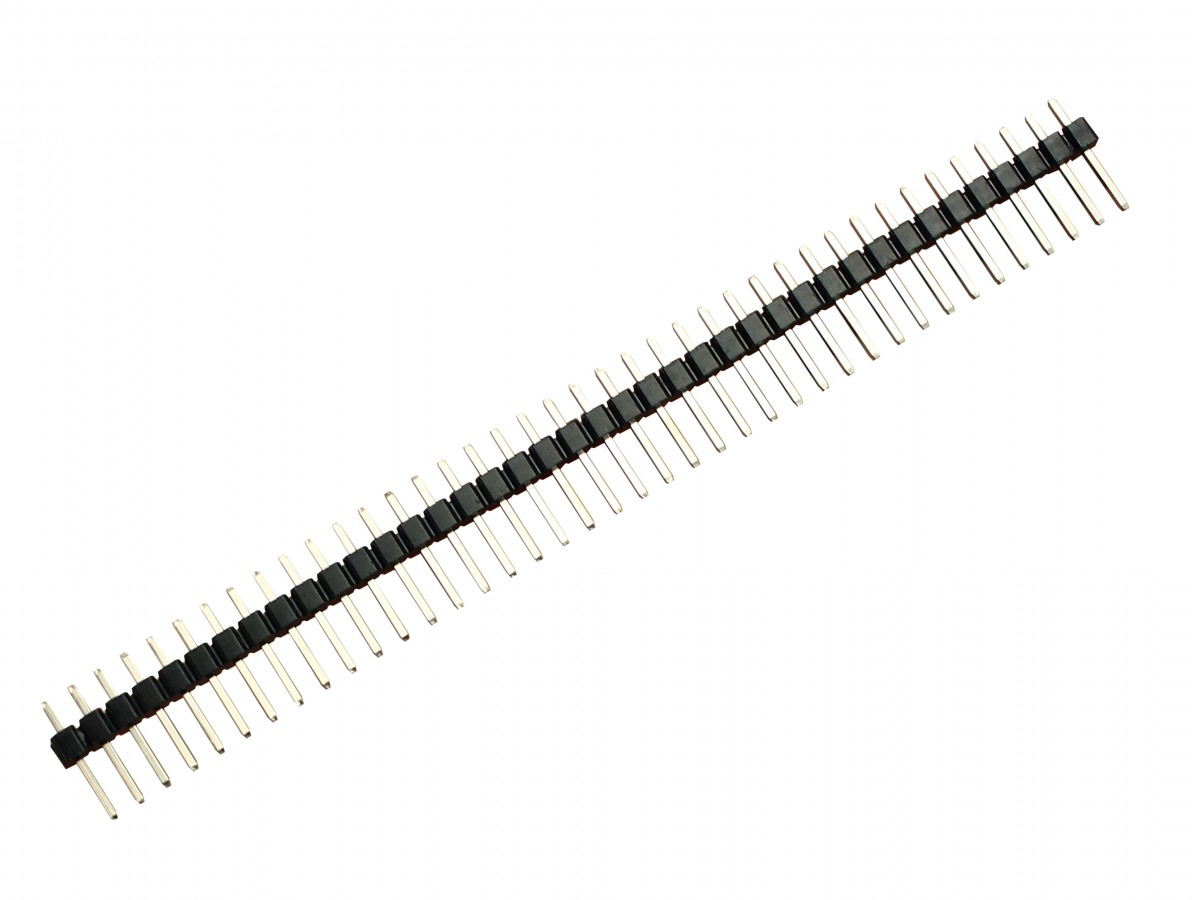
\includegraphics[width=\linewidth, height=6cm]{Imagens/barramacho.jpg}
        \smallcaption{Fonte: \textcite{barrapinomacho}.}
        \label{fig:barramacho}
    \end{minipage}\hfill
    \begin{minipage}{0.45\textwidth}
        \caption{Barra de pinos de tipo fêmea}
        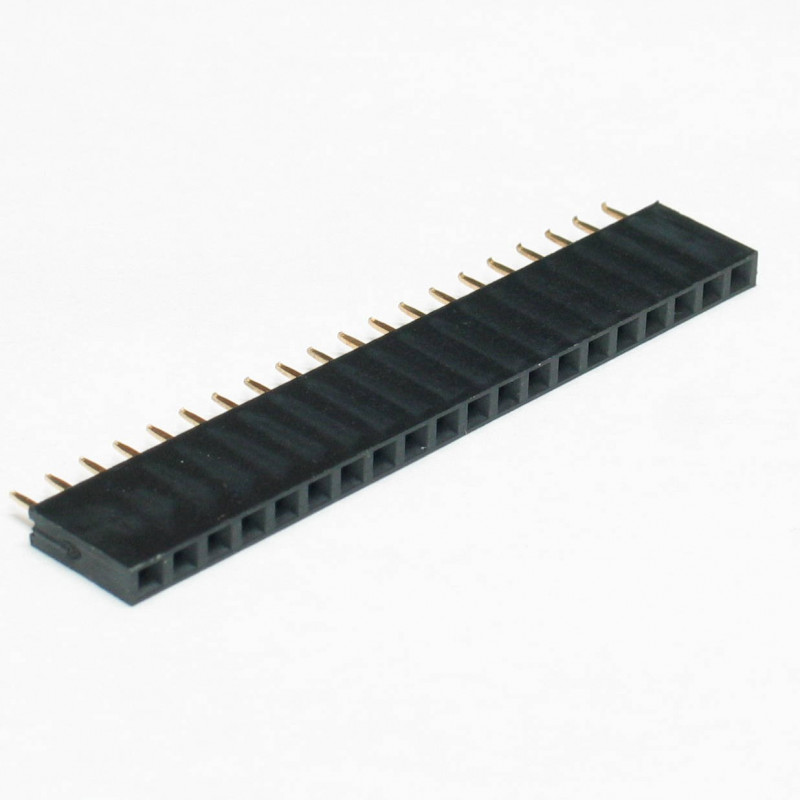
\includegraphics[width=\linewidth, height=6cm]{Imagens/barrafemea.jpg}
        \smallcaption{Fonte: \textcite{barrapinofemea}.}
        \label{fig:barrafemea}
    \end{minipage}
\end{figure}

Sabendo que as \textit{PCBs} precisavam de uma fonte correta de alimentação, pois não utilizavam a energia diretamente da bateria do carro, foi utilizado para o Kit Conforto um módulo de adaptação \textit{Micro USB}, Figura \ref{fig:micro_usb}, previsto também na \textit{footprint} do mesmo e funcionando basicamente como uma entrada de energia comum, assim como a vista em alguns modelos de celular, podendo receber carga elétrica de fontes externas reguladas como as baterias externas portáteis citadas na seção \ref{Proto}. Este módulo \textit{Micro USB} foi selecionado somente para o Kit Conforto, pois o mesmo apresenta três sensores diferentes, além do módulo de \textit{cartão SD}, assim é considerado uma boa prática não utilizar a entrada \textit{Mini USB} própria do \textit{Arduino Nano} como a principal fonte de energia de modo a não sobrecarregar o regulador de tensão presente o microcontrolador. Este não é o caso do Kit Pressão, que possui apenas o sensor de pressão barométrica e o módulo de \textit{cartão SD}, sendo assim não há problema em alimentá-lo com a tensão oriunda da conexão na porta \textit{Mini USB} do \textit{Arduino}.

\begin{figure}[!htb]
\centering
    \caption{Módulo Adaptador Micro \textit{USB} Fêmea para \textit{DIP}}
    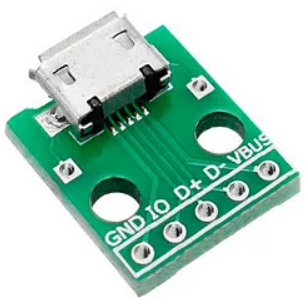
\includegraphics[width=0.25\linewidth]{Imagens/Micro_USB.png}
    \smallcaption{Fonte: \textcite{micro_usb}.}
    \label{fig:micro_usb}
\end{figure}

Torna-se válida também uma breve explicação a respeito do método utilizado para obtenção das placas de circuito impresso. Inicialmente, parte-se da geração de uma máscara contendo o desenho do padrão que se deseja imprimir na placa, que originalmente nada mais é do que uma base vazia para a \textit{PCB}, comumente composta por um polímero com um dos lados completamente recoberto por material com alta condutividade elétrica, sendo um dos mais utilizados o cobre. Definido o padrão desejado, a máquina de Controle Numérico por Computador (CNC) realiza a remoção estratégica de material, deixando trilhas que conectam os componentes e suas respectivas cavidades, onde foram inseridos e posteriormente soldados \cite{sousaPCB}.  

A partir dos desenhos das \textit {footprints}, foi novamente utilizado o software \textit{KiCAD} de modo a se obter a máscara citada em um formato conveniente para ambos os kits, conforme visto nas Figuras \ref{fig:mascaraconfort} e \ref{fig:mascarapressao}, que foram posteriormente enviadas à ferramenta presente no Centro Universitário FEI, por fim realizando a usinagem das trilhas requeridas nas placas. Os passos seguintes consistem na separação das placas uma das outras, já que saem no mesmo conjunto, seguida da soldagem das barras de pinos tipo fêmea nas trilhas.

\begin{figure}[!htb]
    \centering
    \begin{minipage}{0.45\textwidth}
        \caption{Máscara para produção do \textit{PCB} do Kit Conforto}
        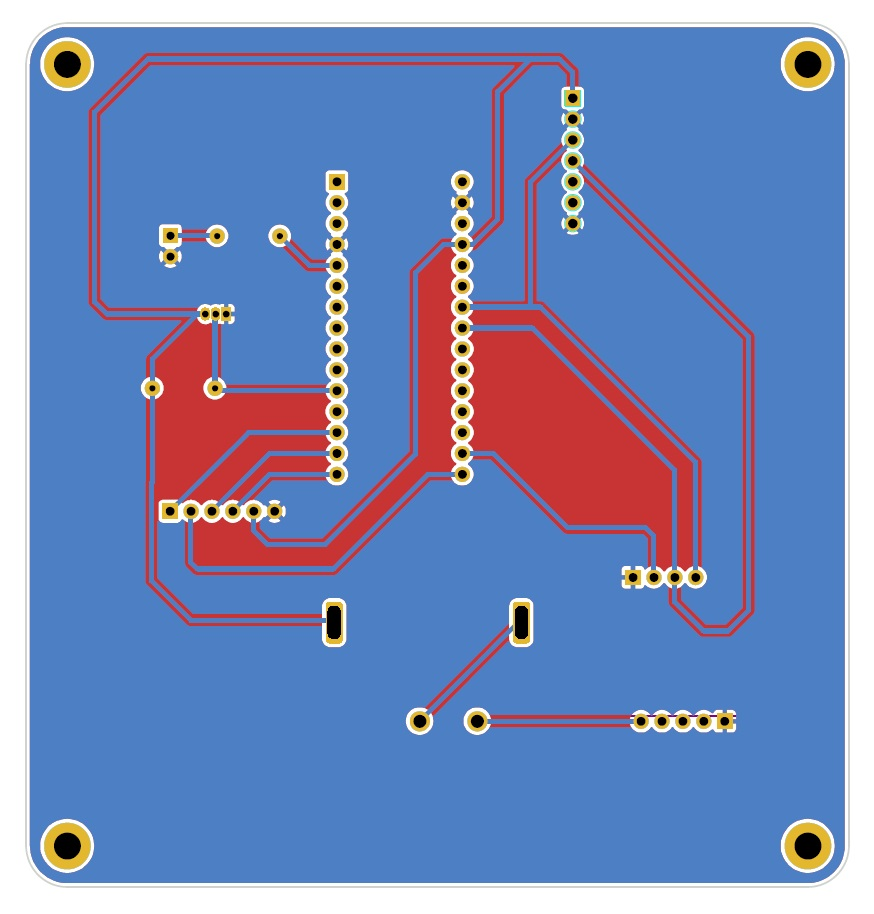
\includegraphics[width=\linewidth, height=7.5cm]{Imagens/mascaraconforto.jpg} 
        \smallcaption{Fonte: Autor.}
        \label{fig:mascaraconfort}
    \end{minipage}\hfill
    \begin{minipage}{0.45\textwidth}
        \caption{Máscara para produção do \textit{PCB} do Kit Pressão}
        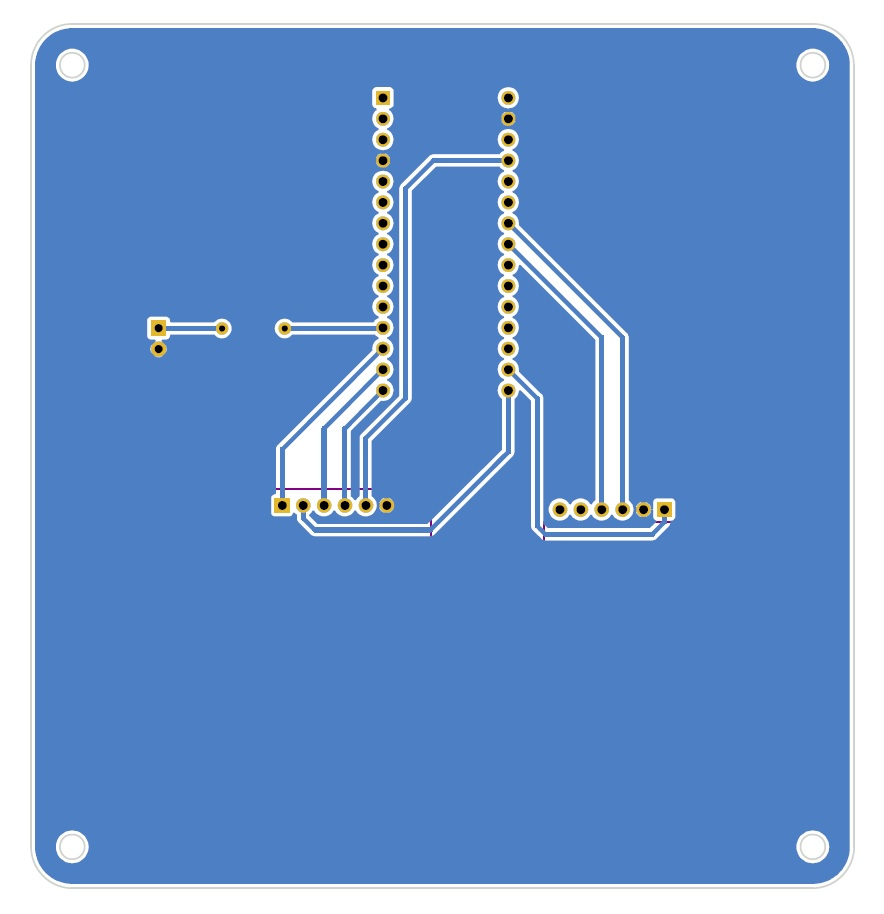
\includegraphics[width=\linewidth, height=7.5cm]{Imagens/mascarapressao.jpg} 
        \smallcaption{Fonte: Autor.}
        \label{fig:mascarapressao}
    \end{minipage}
\end{figure}

Visto que o consumo de corrente do conjunto de microcontrolador e componentes escolhidos é relativamente baixo como foi comprovado pelos testes do grupo e exposto nos \textit{datasheets} dos mesmos, foram escolhidos três modelos de bancos de bateria que os integrantes do grupo já possuíam, com capacidade total das baterias de $8800$, $10000$ e $14000$ \textit{mAh}, valores muito acima da necessidade ao se considerar o consumo de fato observado. Deste modo, a partir dos fatos argumentados, é possível apresentar as Figuras \ref{fig:PCB_conforto} e \ref{fig:PCB_Pressao}, onde são expostas uma das três placas montadas para o Kit Conforto conectado a um dos \textit{Power Banks}, com as luzes do \textit{Arduino Nano} acesas indicando seu funcionamento, exercendo sua função de coleta e armazenamento de dados, e o modelo 3D do Kit Pressão, também oriundo do \textit{KiCAD}, onde as barras de pinos fêmea nomeadas de J2 e J3, da esquerda para a direita, representam os locais onde são conectados o módulo de \textit{cartão SD} e o sensor de pressão, respectivamente.

\begin{figure}[!htb]
\centering
    \caption{\textit{PCB} do Kit Conforto}
    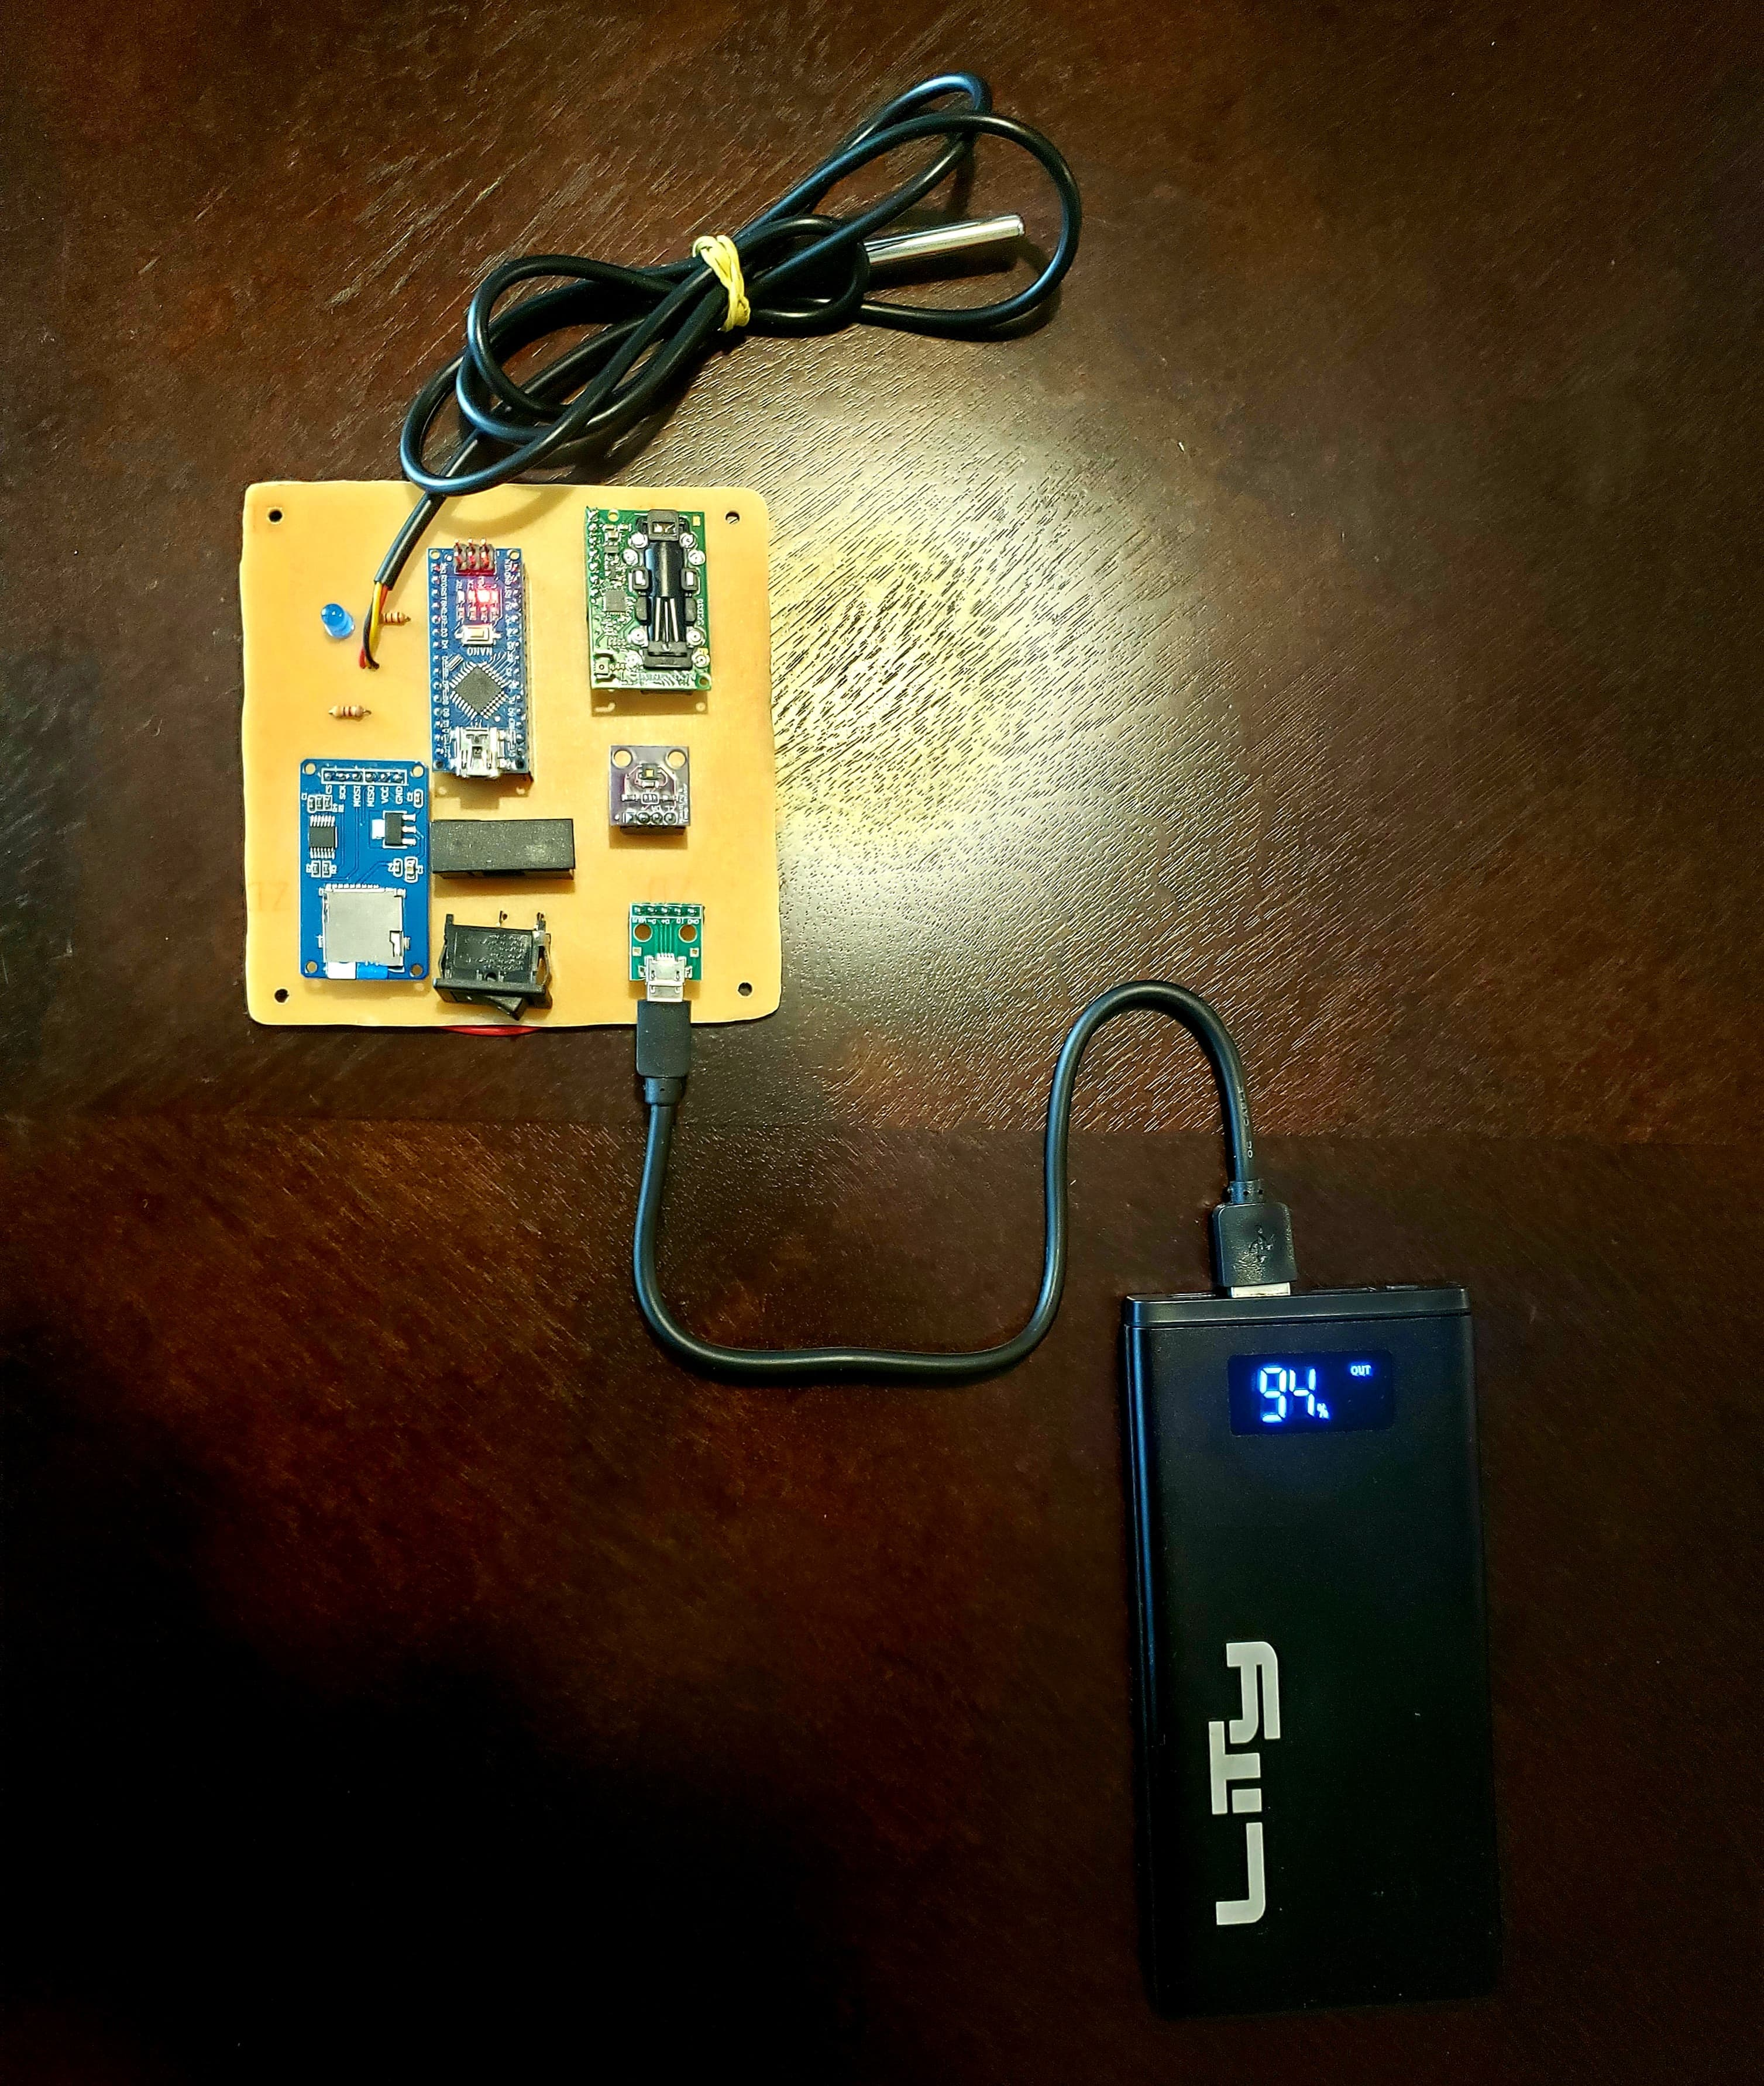
\includegraphics[width=0.5\linewidth]{Imagens/PCB_Conforto.jpeg}
    \smallcaption{Fonte: Autor.}
    \label{fig:PCB_conforto}
\end{figure}

\begin{figure}[!htb]
\centering
    \caption{\textit{PCB} do Kit Pressão}
    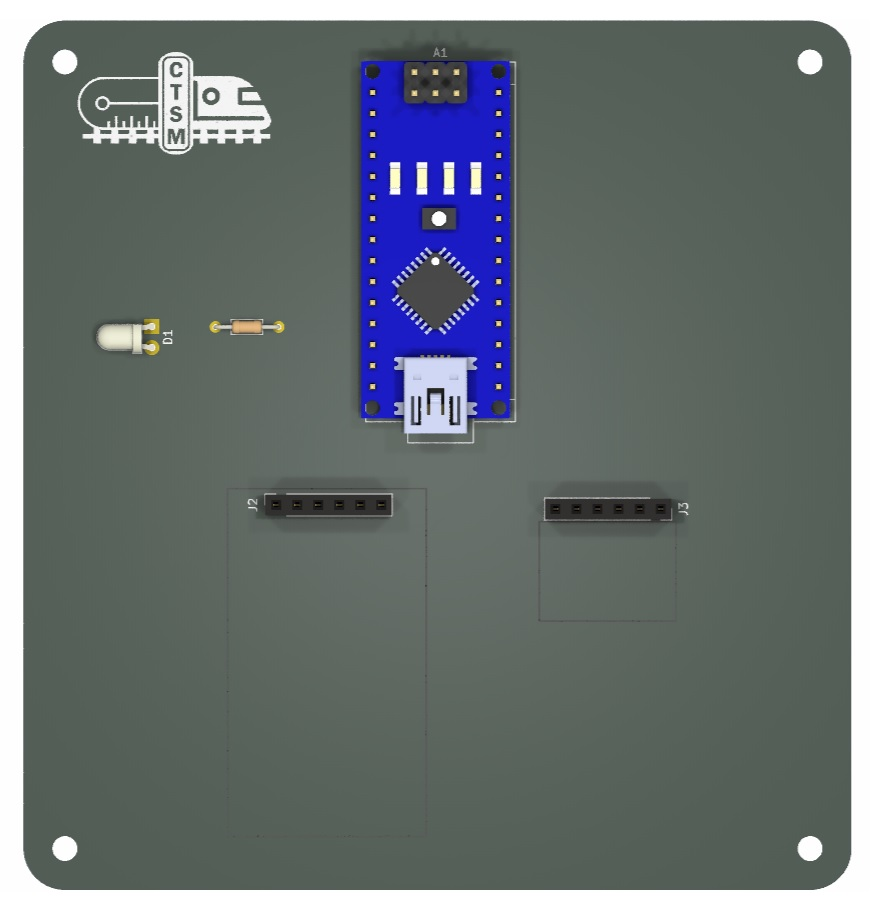
\includegraphics[width=0.4\linewidth]{Imagens/PCB_Pressao.jpg}
    \smallcaption{Fonte: Autor.}
    \label{fig:PCB_Pressao}
\end{figure}

\newpage
Um ponto relevante a se comentar diz respeito à \textit{PCB} do Kit Pressão. Devido a alguns imprevistos, a \textit{PCB} deste kit não estava pronta a tempo da visita marcada com o Metrô de São Paulo para realização das medições. Visto que os dados de pressão devem ser coletados simultaneamente com os de umidade relativa para execução correta dos cálculos de umidade absoluta, tornou-se imprescindível realizar esta medição no dia definido, sob risco de atrasar uma coleta que teria de ser remarcada, o que poderia afetar negativamente o cronograma do grupo. Assim, a \textit{PCB} em questão acabou por não ser produzida, visto que as medições já haviam seguido corretamente apenas com o uso da \textit{protoboard}, situação longe do ideal, mas que mesmo assim conseguiu ser executada com sucesso pelo grupo.


\section{Instrumentação do carro} \label{instruvagao}

Para a adequada análise do sistema de condicionamento de ar no Metrô de São Paulo, foi desenvolvida uma estratégia de instrumentação que visa garantir a máxima precisão na coleta de dados. Após reuniões com o time técnico do Metrô de São Paulo, os pontos de instalação dos sensores foram definidos de forma estratégica, com o intuito de assegurar a melhor qualidade na aquisição de dados, essencial para o sucesso da pesquisa, mas também levando em consideração as limitações impostas ao grupo de modo a não prejudicar os passageiros do serviço.

A respeito das reuniões em questão, é valido comentar sobre as visitas que ocorreram por parte do grupo ao pátio e o que sucedeu em cada uma delas. A primeira ocorreu no dia dezenove de julho de 2024, onde o grupo teve um primeiro contato com todo o ambiente do Metrô de São Paulo, além de conhecer os sistemas mais internos do carro e uma unidade de ar condicionado muito similar à presente no carro selecionado para o estudo, de modo também a já elencar possíveis posicionamentos para os kits de coleta de dados. Entretanto, como o formato final das \textit{PCBs} não estava definido, estas primeiras ideias tiveram de ser alteradas. Depois, com estas informações, o grupo manteve contato constante com a equipe do Metrô, que, sempre muito prestativa, auxiliou a sanar inúmeras dúvidas.

A próxima visita ocorreu no dia 23 de outubro de 2024. Neste dia, a equipe do Metrô retirou de circulação o trem L41, Figura \ref{fig:metrol41}, que foi preparado no pátio Jabaquara para o grupo. Por recomendação dos metroviários, analisaram-se as possibilidades no carro de número 2, classificado como L412, o que permitiu ao grupo uma ideia certeira de onde posicionar as \textit{PCBs}, pois o carro utilizado para as coletas de fato, é idêntico a este modelo. Nesse momento, em posse das \textit{PCBs} do Kit Conforto, o grupo realizou uma análise mais precisa dos locais onde instalar os Kits, sempre com a supervisão e recomendações da equipe.

\begin{figure}[!htb]
\centering
    \caption{Trem L41, estacionado no Pátio Jabaquara}
    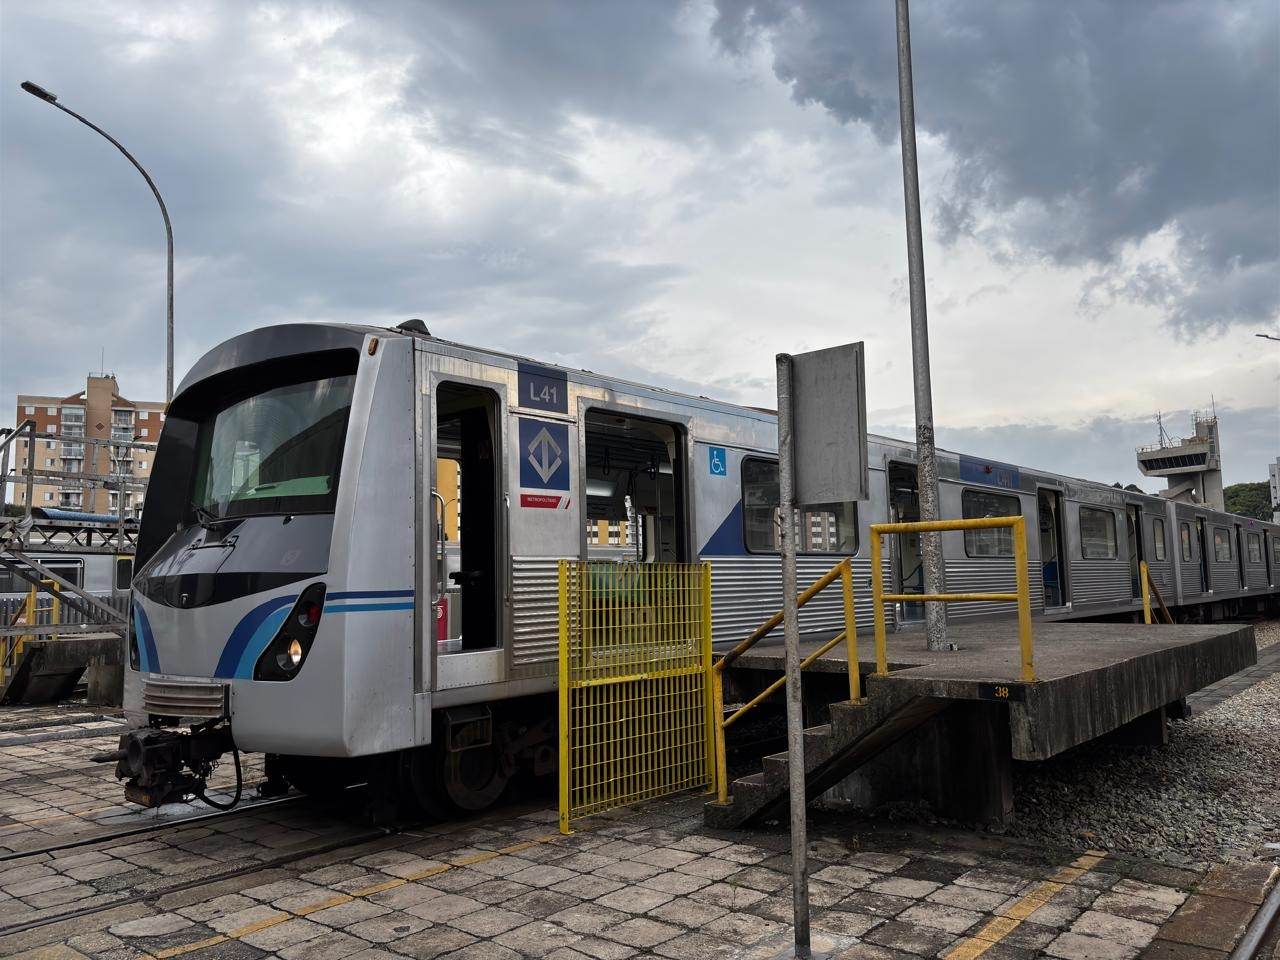
\includegraphics[width=0.60\linewidth]{Imagens/metrol41.jpg}
    \smallcaption{Fonte: Autor.}
    \label{fig:metrol41}
\end{figure}
\newpage
A terceira e última visita ocorreu no dia 25 de outubro do mesmo ano. Aqui, os integrantes do grupo chegaram ao mesmo pátio às quinze horas, com o intuito de preparar os Kits no carro de número 2 do material L28, denominado de L282, Figura \ref{fig:metrol282}, escolhido pela equipe do Metrô, até às dezessete horas, visto que o trem foi retirado logo no início da tarde, onde há menor movimento, mas devia ser devolvido a via ao fim da tarde, onde se inicia um dos horários de pico do dia. Com o auxílio dos metroviários e as informações definidas na visita anterior, além de materiais como tesoura, fita adesiva dupla face, abraçadeiras de \textit{nylon} e suportes de papelão rígido para as \textit{PCBs}, presentes na Figura \ref{fig:matusados}, os Kits e seus respectivos \textit{Power Banks} foram instalados da maneira esperada no carro. 

\begin{figure}[!htp] 
    \centering
    \begin{minipage}{0.45\textwidth}
        \caption{Carro de número 2 do trem L28}
        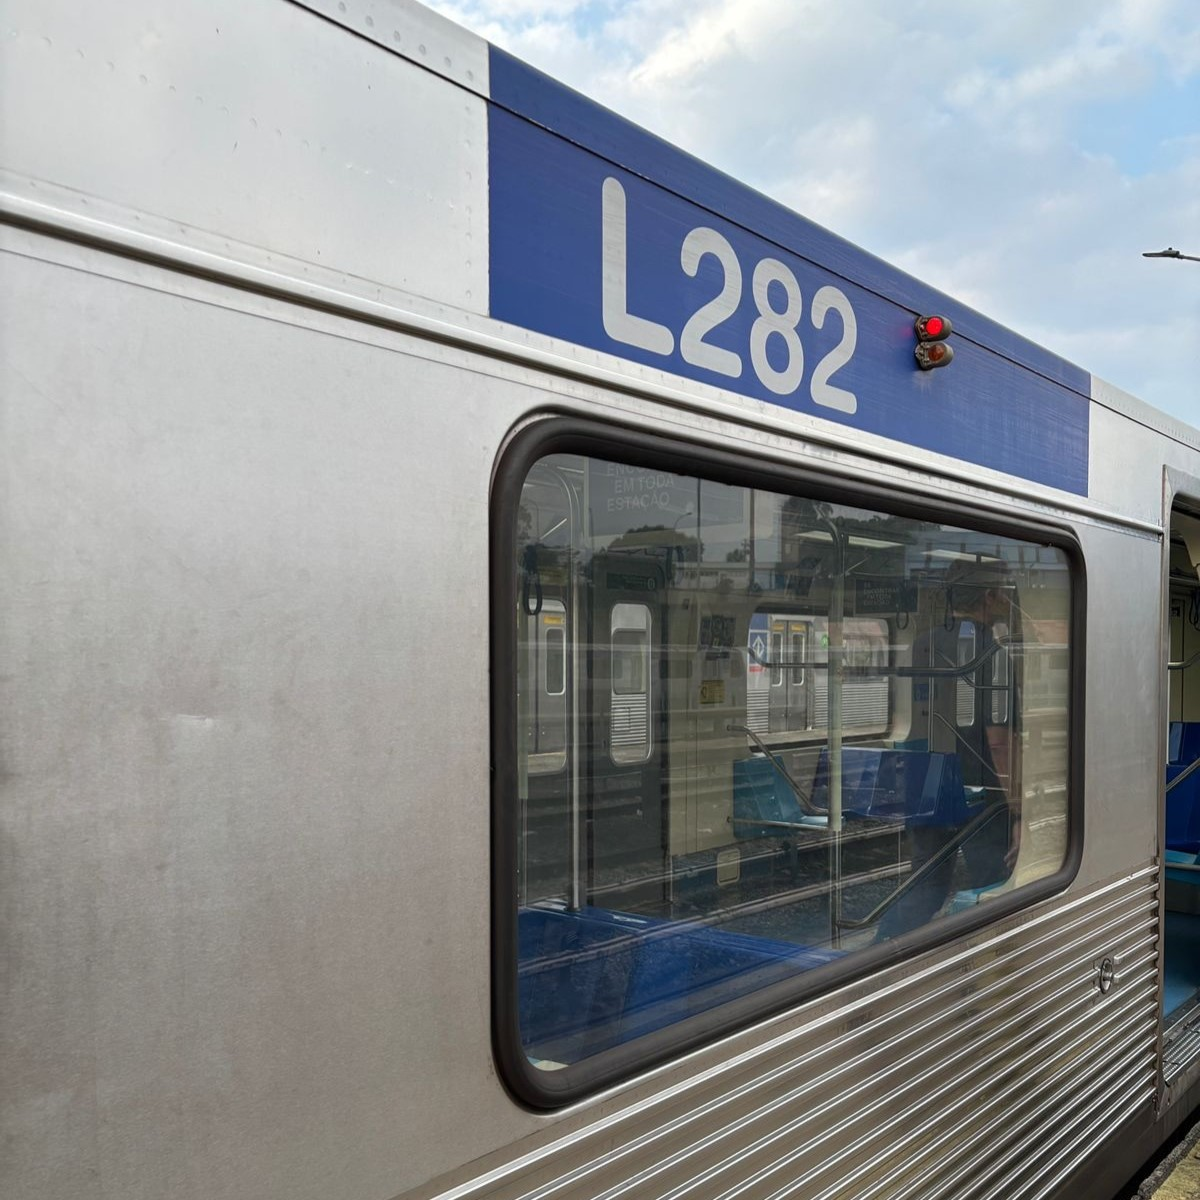
\includegraphics[width=\linewidth, height=7.5cm]{Imagens/metrol282.jpg} 
        \smallcaption{Fonte: Autor.}
        \label{fig:metrol282}
    \end{minipage}\hfill
    \begin{minipage}{0.45\textwidth}
        \caption{Materiais utilizados para fixação dos Kits no carro}
        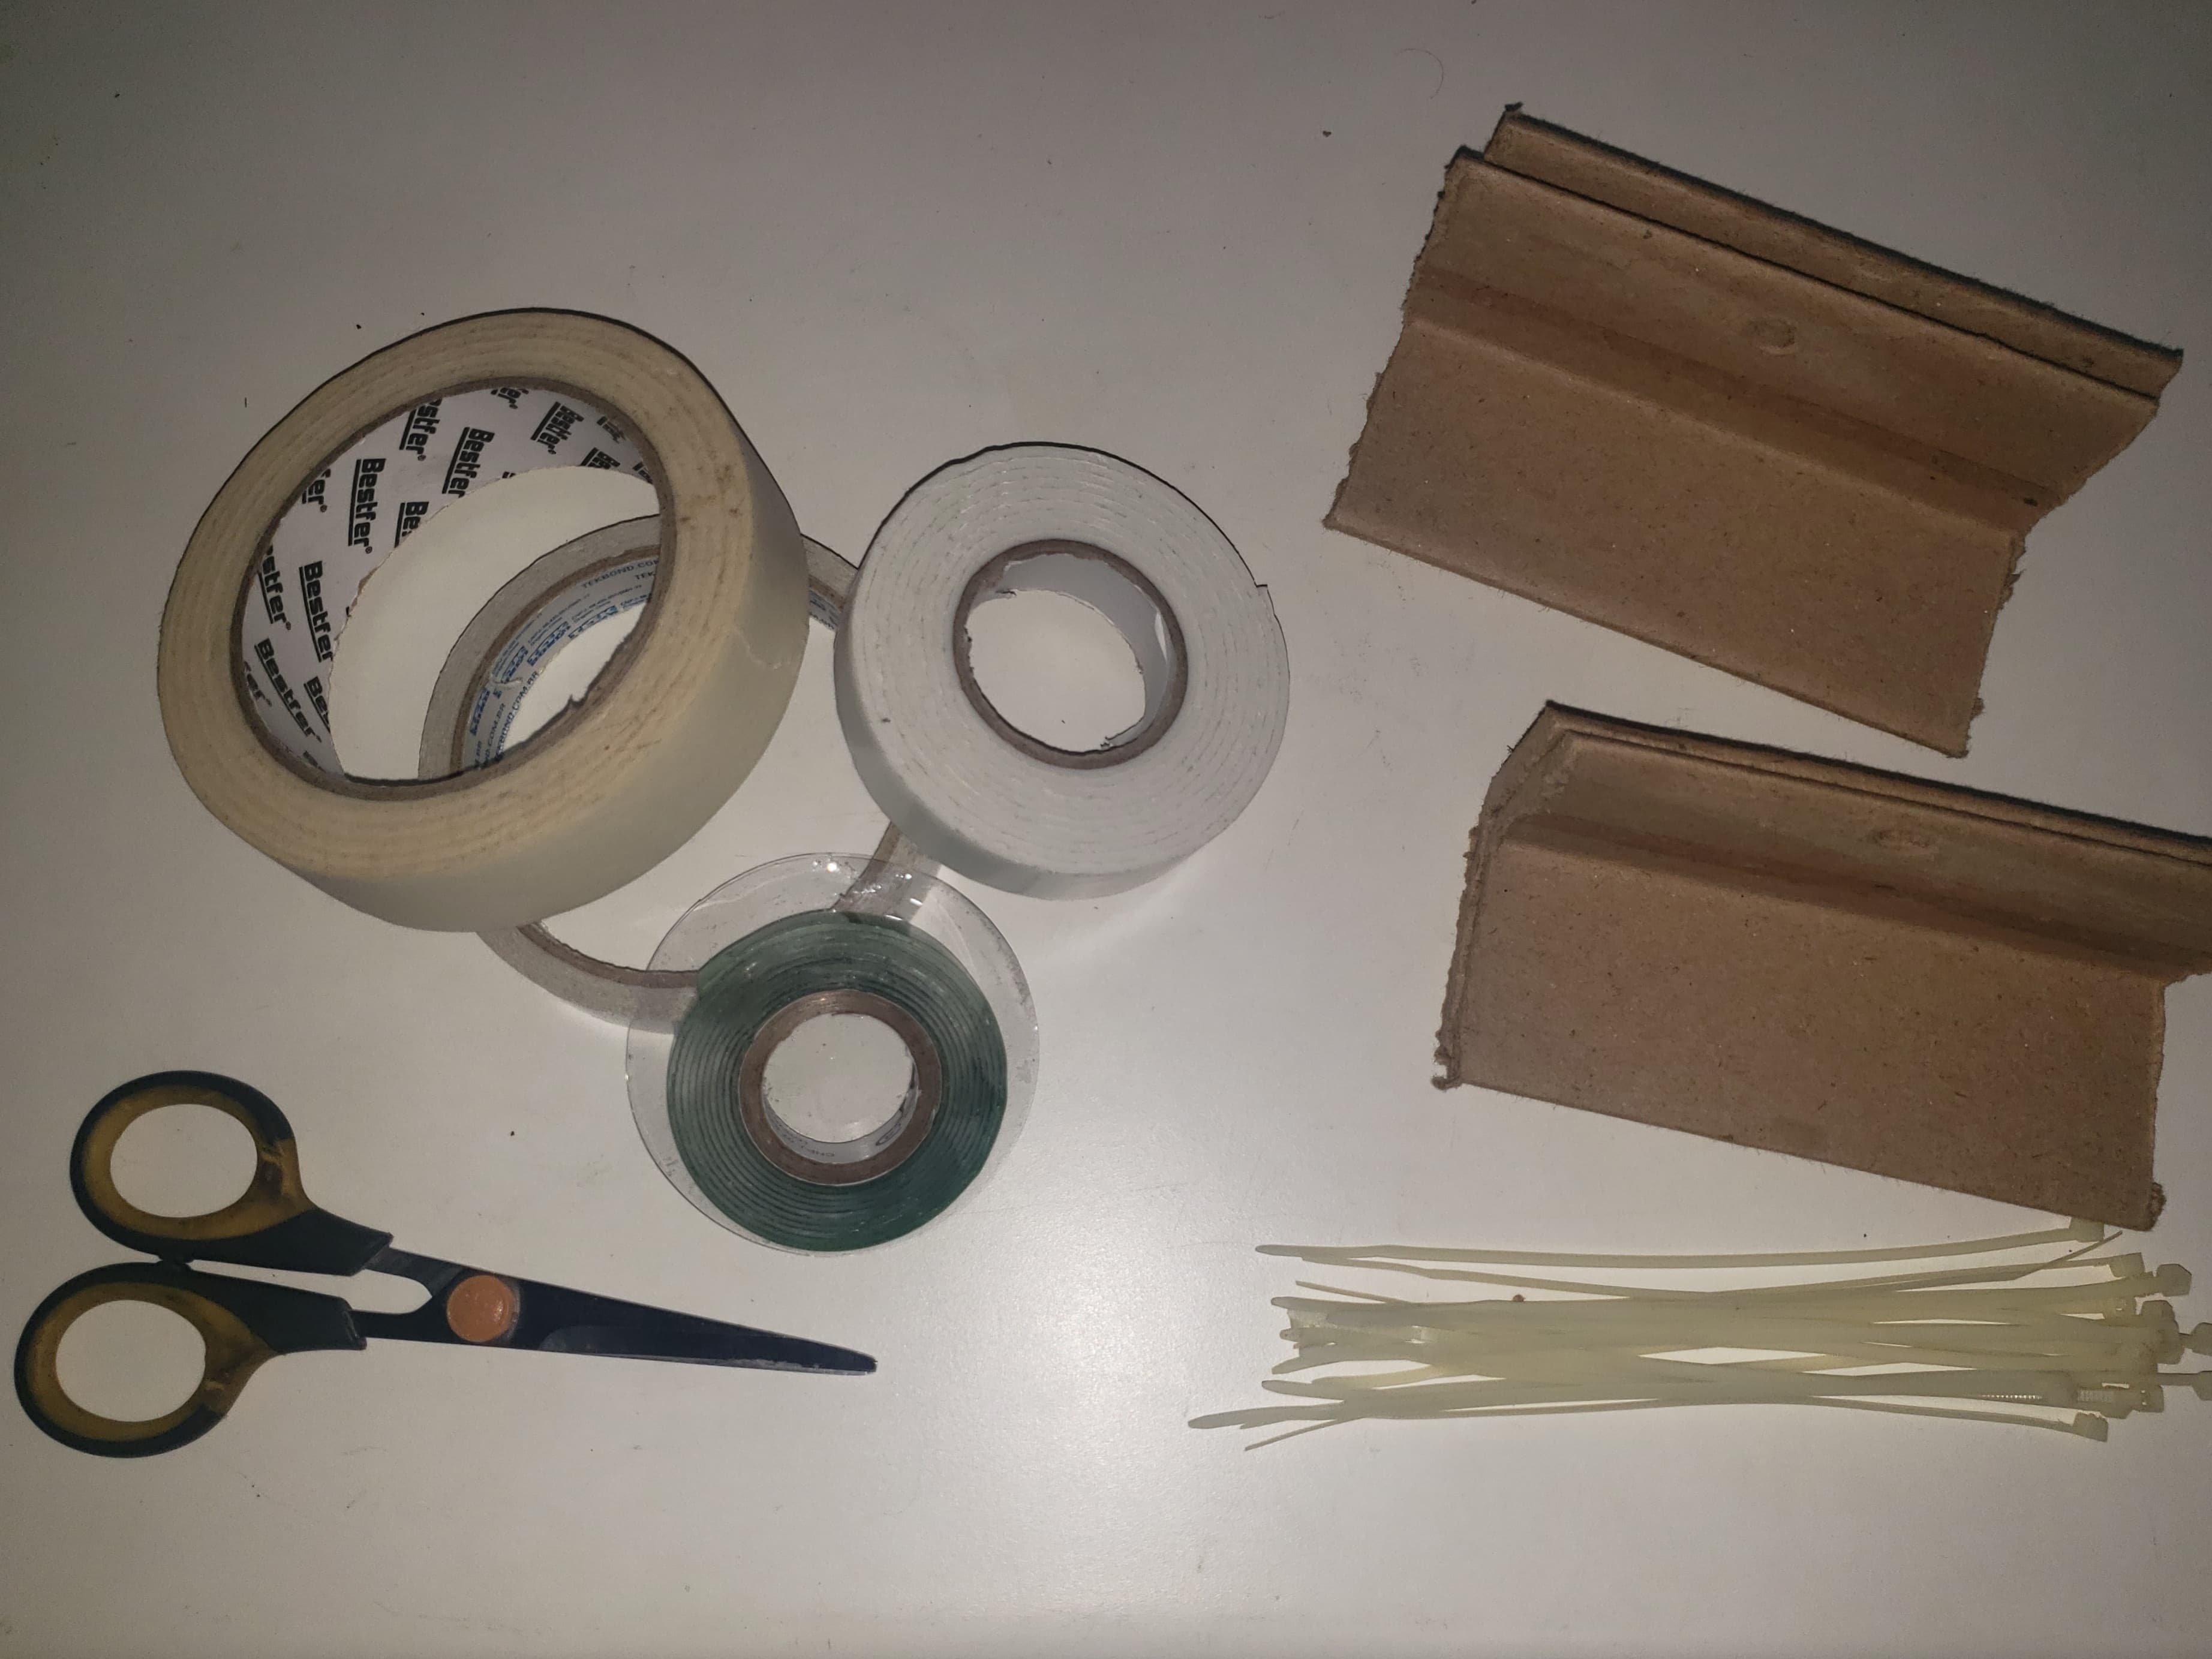
\includegraphics[width=\linewidth, height=7.5cm]{Imagens/matusados.jpeg} 
        \smallcaption{Fonte: Autor.}
        \label{fig:matusados}
    \end{minipage}
\end{figure}

A campanha de medições foi efetuada em um único dia, com coletas realizadas a partir das 16 horas e 44 minutos do dia 25 de outubro de 2024, momento onde todos os kits foram ligados de modo a dar início às suas rotinas de calibração e também já coletando informações sobre o carro vazio, até às 20 horas e 54 minutos do mesmo dia, totalizando 4 horas e 10 minutos de aquisição de dados. É valido comentar também que a primeira estação visitada foi a Jabaquara, às 16 horas e 53 minutos, por haver uma certa distância entre o pátio e a estação. No total foram realizadas 3 voltas completas entre as estações Jabaquara e Tucuruvi.

Esse período de coleta foi definido estrategicamente para que os dados fossem capturados em diferentes momentos de operação do Metrô, abrangendo tanto horários de menor fluxo de passageiros quanto horários de pico com maior lotação. Essa abordagem permitiu uma análise mais robusta e detalhada, uma vez que o comportamento do sistema de climatização pode variar conforme a densidade de ocupação dos carros. A coleta de dados em horários mais vazios e em horários de pico forneceu, portanto, uma visão mais ampla sobre o desempenho do sistema em condições operacionais variadas, o que é essencial para avaliar a eficiência do controle térmico e da qualidade do ar em diferentes cenários de demanda, garantindo assim uma boa assertividade na análise dos dados.

Foram utilizados ao todo quatro kits de medição, distribuídos entre um kit para pressão e três kits para conforto. Os três Kits Conforto iguais, equipados com sensores de temperatura, concentração de dióxido de carbono (${CO}_{2}$) e umidade relativa do ar, foram utilizados para realizar medições em pontos distintos do carro, priorizando a análise da circulação de ar, sendo instalados em pontos próximos ao insuflamento e à exaustão, marcados em verde na Figura \ref{fig:metodo_de_medicao}, visando capturar dados diretamente relacionados ao fluxo de ar-condicionado. Estas PCBs foram posicionadas em áreas estratégicas, sendo elas:

\begin{itemize}[label=\arabic*.]
    \item Monitor próximo ao insuflamento central do carro, geralmente considerado mais gelado pela equipe e passageiros do Metrô. Apresentada na Figura \ref{fig:kittv};
    \item Apoiada em uma barra de apoio ao lado das portas, próxima a um dos pontos de exaustão do ar e margeando a zona afetada pelo insuflamento mencionado no item a. Apresentada na Figura \ref{fig:kitporta};
    \item Base de uma janela na extremidade do carro, sendo este um ponto de medição na altura das pessoas. Apresentada na Figura \ref{fig:kitjanela}.
\end{itemize}

\begin{figure}[!htb]
\centering
    \caption{Kit Conforto instalado em um monitor do Metrô}
    \includegraphics[width=0.39\linewidth]{Imagens/kittv.jpeg}
    \smallcaption{Fonte: Autor.}
    \label{fig:kittv}
\end{figure}

\begin{figure}[!htb]
\centering
    \caption{Kit Conforto instalado acima de uma barra de apoio}
    \includegraphics[width=0.39\linewidth]{Imagens/kitporta.jpeg}
    \smallcaption{Fonte: Autor.}
    \label{fig:kitporta}
\end{figure}

\newpage

\begin{figure}[!htb]
\centering
    \caption{Kits Conforto e Pressão instalados na janela na extremidade do carro}
    \includegraphics[width=0.4\linewidth]{Imagens/kitjanela.jpeg}
    \smallcaption{Fonte: Autor.}
    \label{fig:kitjanela}
\end{figure}


É válido comentar que o Kit Conforto da janela realizou as medições em uma posição ligeiramente inferior aos demais. A intenção é comparar as condições ambientais próximas ao insuflamento e à exaustão com as medições feitas em uma zona mais neutra, onde o ar já está em circulação pelo ambiente. Essa comparação permitirá uma avaliação mais detalhada da distribuição de temperatura, umidade e concentração de ${CO}_{2}$ no carro, fornecendo novas ideias sobre a eficiência do sistema de climatização em diferentes áreas do espaço.

O Kit Pressão, por sua vez, foi instalado no mesmo local que o Kit Conforto na extremidade do carro, conforme ilustrado em amarelo na Figura \ref{fig:metodo_de_medicao} e visto também nas Figuras \ref{fig:kitjanela} e, com mais detalhes, \ref{fig:kitjanelazoom}. O sensor presente no Kit tem a função de medir a pressão barométrica local. A escolha desse posicionamento se justifica pela praticidade no momento da instalação e fixação do kit, além de outras duas questões técnicas. A primeira está ligada simplesmente à quantidade de saídas \textit{USB} encontradas nos \textit{Power Banks}, já que o banco de baterias que possui duas destas saídas foi colocado na janela. A segunda questão diz respeito à construção deste kit. Como mencionado na seção \ref{Proto}, a PCB para esta placa não ficou pronta na data esperada, tornando então necessário o posicionamento mais simples possível para este kit visto que a \textit{protoboard} não apresenta caráter de produto final, isto é, locais mais complexos resultariam em possíveis problemas causados pelas conexões via \textit{jumper} expostas, além de sua facilidade de desconexão acidental, ocasionada por toque não intencionado de algum passageiro do Metrô, ou até mesmo a simples vibração enfrentada pelo carro.

\begin{figure}[!htb]
\centering
    \caption{Visão com maior detalhe dos Kits Conforto e Pressão instalados na janela na extremidade do carro}
    \includegraphics[width=0.50\linewidth]{Imagens/kitjanelazoom.jpeg}
    \smallcaption{Fonte: Autor.}
    \label{fig:kitjanelazoom}
\end{figure}

Dados estes apontamentos, é possível dizer que a abordagem metodológica escolhida pelo grupo, validada pelo time técnico do Metrô de São Paulo, visa proporcionar uma visão detalhada e suficientemente precisa das condições de operação do sistema de ar-condicionado, mesmo em condições não ideais como a exposta com o caso do Kit Pressão, contribuindo para otimizar o conforto dos passageiros e a eficiência energética dos sistemas de climatização. 

\section{Dados fornecidos pelo Metrô de São Paulo}

Os dados recebidos através da equipe do Metrô de São Paulo são essenciais para o estudo realizado, por possibilitarem uma contextualização das condições atuais do sistema. Além disso, são dados necessários para a realização dos cálculos teóricos, desenvolvimento das simulações fluidodinâmicas e para a análise estatística dos dados. Nesse sentido, seria inviável realizar modelagens e cálculos precisamente a partir de dados que não refletem diretamente as condições atuais do sistema de ar-condicionado.

Visando fundamentar o estudo realizado, foram recebidos dados diretamente do Metrô de São Paulo, que permitiram uma análise mais aprofundada do problema. A equipe responsável forneceu a temperatura de exaustão e insuflamento do carro, o peso dos carros e as reclamações dos passageiros direcionadas ao funcionamento do Metrô, além de esquemáticos e desenhos do carro. 

\subsection{Peso dos Carros} 

    A medição de peso nos carros do Metrô de São Paulo é efetuada através das bolsas de ar do sistema de suspensão, localizadas nos “truques". As bolsas ajustam a altura do carro, ajustando o nível conforme o peso a ser transportado. O sistema pneumático, alimentado por um compressor, é responsável por fornecer o ar comprimido para as bolsas, que por sua vez são controladas por válvulas niveladoras. Essas válvulas mantêm a pressão balanceada nas bolsas. Por sua vez, os transdutores de pressão presentes no sistema pneumático possibilitam direcionar os dados para o sistema eletrônico do trem.
    
    A pressão nas bolsas de ar de carro está diretamente ligada ao número de passageiros. Com isso, a pressão é convertida para um valor em toneladas, o que pode ser convertido posteriormente para um número aproximado de pessoas presentes no carro. Exemplificando, a partir do peso em toneladas do carro, pode-se estimar o número de pessoas presente no carro em determinado horário, por exemplo, uma pressão correspondente a duas toneladas de peso indica que existem aproximadamente 30 pessoas no carro, considerando um peso médio por pessoa de $70$ $kg$.
    
    No contexto apresentado, o peso do carro foi utilizado para estimar o número aproximado de pessoas, visto que a equipe do Metrô de SP não possuía a informação do número exato de pessoas por carro, sendo uma informação valiosa para o tratamento e análise de dados realizados. É importante mencionar que, por se tratar de um conteúdo confidencial, não foi permitida a divulgação do diagrama do sistema pneumático do Metrô.
    
    Dessa maneira, foram recebidas planilhas através da equipe do Metrô de SP contendo o peso dos carros da frota L medido pelo sistema descrito anteriormente \cite{metrosp2024}. Como é possível observar na Figura \ref{fig:Peso_Carros}, o carro número $5$ passou de $12$ toneladas para $9$ toneladas, ou seja, aproximadamente $43$ pessoas desembarcaram do trem, considerando um peso médio de pessoa de $70$ $kg$.
    
    \begin{figure}[!htb]
    \centering
    \caption{Peso em Cada carro da frota L}
    \includegraphics[width=1\linewidth]{Imagens/Peso_Carros.png}
    \smallcaption{Fonte: \textcite{metrosp2024}.}
    \label{fig:Peso_Carros}
    \end{figure}

\subsection{Temperatura interna e externa do carro} 
     
    Foram recebidos dados dos sensores de temperaturas já presentes no carro, localizados entre o salão e o filtro, sendo no caso a temperatura de exaustão. Essas informações foram utilizadas na análise, permitindo a construção de gráficos e tratamento de dados. Além disso, foi utilizada de maneira comparativa, visando validar o funcionamento dos sensores de temperatura instalados para o sensoriamento \cite{metrosp2024}. 

    O Metrô de São Paulo possui dois sensores de temperatura instalados, um de exaustão, localizado entre o salão e o filtro do ar condicionado, e outro fixado na parte externa do carro. Dessa maneira, pode-se dizer que o sensor interno não representa de maneira verdadeira a temperatura na área na qual as pessoas circulam, não oferecendo dados muito precisos do sistema a ser estudado, apenas servindo de referência para o estudo. A Figura \ref{fig:Sensor_Exaustao_Metro} representa a localização do sensor de temperatura de exaustão do Metrô, situando-se na região na qual o ar passou pela grelha de exaustão e direciona-se à evaporadora, misturando-se com o ar externo.
    
     \begin{figure}[!htb]
    \centering
    \caption{Localização do sensor de temperatura de exaustão do Metrô}
    \includegraphics[width=1\linewidth]{Imagens/Sensor_Exaustao_Metro.png}
    \smallcaption{Fonte: Autor.}
    \label{fig:Sensor_Exaustao_Metro}
    \end{figure}   
    
\newpage
    Os sensores utilizados pela empresa são sensores de temperatura \textit{E52-E} que podem ser observados na Figura \ref{fig:Sensores_Metro}. Esses sensores possuem uma vasta gama de opções para o alojamento, facilitando montagem e ligação. Além disso, possui ótima correspondência de desempenho como controlador térmico. Como é possível observar na Figura \ref{fig:Temperatura_Carros}, é possível ver todas as temperaturas de exaustão e externa, para cada carro.
    
    
    \begin{figure}[!htb]
    \centering
    \caption{Sensores de Temperatura Utilizados pelo Metrô de SP}
    \includegraphics[width=0.6\linewidth]{Imagens/Sensor_Metro.jpg}
    \smallcaption{Fonte: \textcite{metrosp2024}.}
    \label{fig:Sensores_Metro}
    \end{figure}

    \begin{figure}[!htb]
    \centering
    \caption{Temperatura em Cada carro da frota L}
    \includegraphics[width=1\linewidth]{Imagens/Temperatura_Carros.png}
    \smallcaption{Fonte: \textcite{metrosp2024}.}
    \label{fig:Temperatura_Carros}
    \end{figure}

\subsection{Reclamações dos passageiros da frota L}

    As reclamações dos passageiros da frota foram adquiridas através do portal de reclamações do Metrô, no caso, o “SMS-Denúncia”, sendo um serviço que possibilita que os passageiros do Metrô denunciem irregularidades ou façam reclamações sobre ocorridos no carro. Tendo isso em vista, para realizar a denúncia, a pessoa deve descrever o acontecimento, informando a linha, o número do carro e a estação. 
    
    A equipe do Metrô forneceu planilhas contendo as reclamações referentes ao ar-condicionado, que possuem dados organizados por dia e horário, natureza da reclamação, número do trem e do carro, além do número da via, como é possível observar na Figura \ref{fig:SMS_Denuncia}. Esses dados foram utilizados no estudo estatístico que, em conjunto com os outros segmentos do trabalho, possibilitou a análise e tratamento de dados, juntamente com a proposição de melhorias \cite{metrosp2024}.
    
\begin{figure}[!htb]
    \centering
    \caption{Trecho da Planilha das Reclamações da frota L}
    \includegraphics[width=1.0\linewidth]{Imagens/SMS_Denuncia.png}
    \smallcaption{Fonte: Autor.}
    \label{fig:SMS_Denuncia}
\end{figure}


\subsection{Esquemáticos e desenhos do carro} 
    
Durante o desenvolvimento do trabalho, foram recebidos desenhos 2D e esquemáticos do Metrô e do sistema de ar-condicionado, contendo detalhes técnicos a respeito da geometria e estrutura dos carros e do ar condicionado. Esses documentos são essenciais para a realização de uma análise coesa, tanto dos processos de troca térmica quanto das simulações fluido dinâmicas. A partir dos desenhos 2D recebidos, foram desenvolvidos modelos 3D utilizados para as simulações e para definir a geometria adotada para o carro. É importante mencionar que, por se tratar de um conteúdo confidencial, não foi permitida a divulgação do material, juntamente com a divulgação das dimensões exatas do carro.
 
\section{Conforto Térmico}

Como dito nas premissas do projeto e nas simplificações, a \textcite{ASHRAE2009} tem algumas normas que ditam o conforto térmico. O estudo do conforto térmico é importante porque avalia a condição do ambiente e, também, como as pessoas percebem e sentem o ambiente. Apesar de ser uma condição mental e ser muito subjetivo, ainda é possível prevê-lo por meio de um voto médio de previsão (\textit{PMV}).

O \textit{PMV} se baseia na escala de conforto da \textit{ASHRAE} mostrada na Tabela \ref{tab: conforto} a qual varia entre $\pm3$, onde $-3$ significa muito frio, $+3$ muito quente e o 0 neutro. Para um ambiente ser considerado termicamente confortável, o valor de seu \textit{PMV} precisa estar o mais próximo de 0 possível, podendo ser considerado conforto térmico a partir de $\pm$ 0,5.

Juntamente com o \textit{PMV}, existe o \textit{PPD}, que mede, em porcentagem, a insatisfação das pessoas por meio do voto de percepção. Esse valor nunca será zero, pois mesmo que o voto de percepção esteja neutro, na escala, $5\%$ das pessoas ainda estarão insatisfeitas.
   
    
\section{Simulações Fluido Dinâmicas} \label{Simulacao}

Neste tópico, foram abordados os modelos e parâmetros utilizados para o desenvolvimento das simulações fluido dinâmicas através do \textit{software Ansys}. Descrevem-se em detalhes as condições de contorno, o refinamento da malha e as simplificações adotadas para viabilizar as análises realizadas, garantindo que o sistema se comporte de maneira adequada, representando um modelo próximo à situação real.

Em uma primeira etapa do desenvolvimento, foi realizada a modelagem do primeiro desenho 3D, observado na Figura \ref{fig:Desenho_Metro}, sendo utilizado como modelo preliminar para indicar a geometria do ambiente estudado. Porém, por falta de poder computacional, foram necessárias simplificações para utilizá-lo nas simulações fluido dinâmicas, permitindo resultados suficientes para análise.

\begin{figure}[!htb]
    \centering
    \caption{Desenho 3D Preliminar}
    \includegraphics[width=0.8\linewidth]{Imagens/Desenho_Metro.png}
    \smallcaption{Fonte: Autor.}
    \label{fig:Desenho_Metro}
\end{figure}

 No carro, foram consideradas 48 pessoas sentadas e 70 em pé, como pode ser observado na Figura \ref{fig:PessoasXZ}. Vale mencionar que foram consideradas variações de altura para as pessoas, simplificadas para paralelepípedos retos de base quadrada. A Tabela \ref{tab:imagem_variacao_altura} mostra a quantidade de pessoas utilizadas e suas alturas.

\begin{figure}[!htb]
    \centering
    \caption{Distribuição das pessoas no carro}
    \includegraphics[width=0.8\linewidth]{Imagens/pessoasazul.png}
    \smallcaption{Fonte: Autor.}
    \label{fig:PessoasXZ}
\end{figure}

\begin{table}[!htb]
    \centering
    \caption{Variação de Altura Simulação}
    \includegraphics[width=0.4\linewidth]{Imagens/imagem_variacao_altura.png}
    \smallcaption{Fonte: Autor.}
    \label{tab:imagem_variacao_altura}
\end{table}


\newpage
Adicionalmente, pode-se observar na Figura \ref{fig:inlet-outlet} os pontos de insuflamento e de exaustão, respectivamente. Essas geometrias representam as grelhas presentes no carro, permitindo emular a entrada e saída de ar do carro no sistema estudado.

\begin{figure}[!htb]
    \centering
    \caption{Pontos Insuflamento e Exaustao}
    \includegraphics[width=0.8\linewidth]{Imagens/inlet-outlet.png}
    \smallcaption{Fonte: Autor.}
    \label{fig:inlet-outlet}
\end{figure}


Para efetuar a simulação, foi necessário ativar o recurso de gravidade no \textit{Ansys}, pois sem este parâmetro ativado não seria possível emular a movimentação do ar no carro. Além disso, como modelo de turbulência foi escolhido o “k-ômega”, sendo o mais apropriado para escoamentos com alta ou média turbulência. Para o cálculo efetuado pelo \textit{software} foram consideradas $200$ interações, visando obter uma boa representação do problema e poupar trabalho computacional desnecessário. Por se tratar de um sistema que representa um escoamento turbulento, não ocorre convergência.

Em relação às condições de contorno, foram consideradas velocidade de $1,28$ $m/s$ e temperatura de $18,42\space ^\circ C$, no insuflamento e pressão de $0$ $Pa$ e temperatura de $21,55\space^\circ C$. É importante destacar que esses valores foram obtidos a partir do sensoriamento realizado no carro da frota L. A Tabela \ref{tab:condicoescontorno} mostra, resumidamente, os parâmetros utilizados. 

\begin{table}[!htb]
    \centering
    \caption{Condições de contorno}
    \includegraphics[width=0.4\linewidth]{Imagens/condicoescontorno.jpeg}
    \smallcaption{Fonte: Autor.}
    \label{tab:condicoescontorno}
\end{table}

Para os parâmetros referentes às pessoas, foi considerado um coeficiente de transferência de calor (h combinado de convecção e radiação) de $16,36$ $W/(m^2K)$. A temperatura do fluido foi de $21,5\space^\circ C$, valor este retirado das medições com os sensores. A temperatura radiante teve seu valor simplificado para o valor da temperatura da pele, sendo de $33,24 \space^\circ C$. Além disso, foi considerada uma emissividade de 0,95 e uma taxa de geração de calor para as pessoas de $368,1$ $W/m^3$. É importante ressaltar que, para uma simulação mais realista, foi criado um material para a pele humana. Um resumo dos parâmetros está representado na Tabela \ref{tab:tabelaproppessoas}.

\begin{table}[!htb]
    \centering
    \caption{Modelagem das pessoas}
    \includegraphics[width=0.4\linewidth]{Tabelas/tabelaproppessoas.jpeg}
    \smallcaption{Fonte: Autor. Adaptado de \textcite{ferreira2001modelo}}
    \label{tab:tabelaproppessoas}
\end{table}

\newpage

Foi preciso especificar, também, as propriedades do ar no \textit{software}, visando uma simulação do sistema próxima à situação real. Portanto, o ar foi considerado como gás ideal, como forma de simplificação. As demais propriedades foram consideradas a partir de um ar a $25\space^\circ C$.

A respeito da malha volumétrica utilizada no estudo, foi utilizada uma geometria poliédrica, que possui um bom custo benefício entre precisão da simulação e trabalho computacional. Além disso, foi adotado um tamanho de malha $0,05$ $m$. As configurações da malha podem ser observadas na Tabela \ref{tab:malhas}.

\begin{table}[!htb]
    \centering
    \caption{Configurações da malha}
    \includegraphics[width=0.5\linewidth]{Tabelas/malhas.jpeg}
    \smallcaption{Fonte: Autor.}
    \label{tab:malhas}
\end{table}

\chapter{Resultados e Discussões}

Neste tópico, foram abordados os resultados obtidos a partir das análises realizadas sobre o condicionamento de ar no carro da frota L do Metrô de São Paulo. Foram discutidos os resultados dos equacionamentos e das simulações fluidodinâmicas, que permitiram uma análise detalhada do comportamento do sistema de ar condicionado do carro em determinadas condições estipuladas. Ademais, foram apresentadas as análises dos dados coletados pelos sensores instalados, realizando correlações com os dados fornecidos pelo Metrô de SP. Estas correlações são fundamentais para validar as simulações e cálculos realizados e para proporcionar uma análise coesa do sistema estudado, seguindo normas de condicionamento de ar. A partir do estudo, foram levantadas sugestões de melhorias e ajustes que permitam otimizar o desempenho do sistema, visando um transporte público mais agradável.

\section{Análise dos dados fornecidos pelo Metrô de São Paulo}

Os dados fornecidos tem alguns componentes importantes a serem analisados, sendo o principal a falta de linearidade, infelizmente os dados fornecidos pelo Metrô de São Paulo estão em escalas de tempo diferentes, logo não é possível fazer nenhuma afirmação assertiva de correlação, porém pode-se criar hipóteses a partir do comportamento dos modelos. A segunda informação importante é que os dados não são do mesmo trem, porém são da mesma frota, sendo ela a frota L (Tucuruvi — Jabaquara).

Foram fornecidos ao trabalho através da parceria com o Metrô de São Paulo, três bases de dados, no formato \textit{CSV}, sendo elas: dados do peso dinâmico do trem em ($t$) do dia 07/11/2023 até 08/06/2024 com um total de 197.204 linhas, dados de temperatura externa e de exaustão do trem em $^{\circ}C$ do dia 28/08/2024 até 20/09/2024 com um total de 23.055 linhas, dados das reclamações de \textit{SMS} do dia 03/01/2023 até 26/08/2024 com um total de 1.274 linhas. Todos os dados, em ordem, são visualizados no fluxograma na Figura \ref{fig:Fluxograma_dos_dados}. A partir desses dados foi possível criar os modelos que foram utilizados para as contas nas seções \ref{equações} e \ref{termico}.

\begin{figure}[!htb]
    \centering
    \caption{Fluxograma dos dados fornecidos pelo Metrô de São Paulo}
    \includegraphics[width=0.8\linewidth]{Imagens/Fluxograma_dos_dados.png} %Tirar particulados
    \smallcaption{Fonte: Autor.}
    \label{fig:Fluxograma_dos_dados}
\end{figure}
\newpage

\subsection{Tratamento de dados} \label{trata}

Com a quantidade de dados excessiva é necessário um tratamento estatístico robusto para assegurar que os modelos a serem gerados a partir dos dados fornecidos são válidos desde sua base. Com isso quatro variáveis foram selecionadas para serem retiradas do banco de dados, os finais de semanas, os feriados, os dados nulos e os \textit{outliers}.

A retirada dos finais de semana e feriados se fez necessária por serem dados não recorrentes, podendo assim causar muito ruído na criação de modelos, pois não representam o padrão de fluxo esperado, logo podem ser retirados nesse momento. Já a remoção dos dados nulos é essencial por serem dados que não são analisáveis, sendo gerados por diferentes falhas como: mal funcionamento momentâneo dos sensores ou leitura do dado em uma frequência diferente da que o sensor opera, entre outros problemas. Existem várias formas de lidar com esses tipos de dados nulos como a especulação de dados através dos seus pares, porém para a criação do modelo, a remoção desses dados se apresenta como a melhor escolha, para manter a base na realidade dos dados. 

Por fim, o último tratamento realizado foi da retirada dos \textit{outliers}. Os \textit{outliers} são valores da amostra que divergem dramaticamente da média, como define \textcite{barnett1994outliers}, um \textit{outliers} é uma observação que desvia muito de outras observações despertando suspeitas de que são geradas por um mecanismo diferente, estas observações são também designadas por anormais, discrepantes, extremas ou aberrantes. Um dos possíveis métodos para identificação desses valores é através do método de \textit{${Z}_{score}$}. Segundo \textcite{curtis2016mystery}, o \textit{${Z}_{score}$}, é um meio de expressar o desvio de uma determinada medida anatômica ou física de uma média populacional específica de tamanho ou idade. O \textit{${Z}_{score}$} descreve quantos desvios-padrão acima ou abaixo de um tamanho de população um valor específico dessa amostra se encontra, esse valor pode ser chamado de \textit{score}, e a forma para obter esse \textit{score} de uma amostra é dada pela Equação \ref{eq:zscore}. Outra forma de observar essa relação é de forma gráfica, como mostra a Figura \ref{fig:zscore}, onde se pode ver que a partir do \textit{score} 3, já representa $99,87\%$ de todos os dados da população. O valor de \textit{score} escolhido para o tratamento dos dados foi o de 10, pois medições de dados muito além da média foram consideradas falhas de medição dos sensores.   

\begin{equation} \label{eq:zscore}
    \begin{aligned}
    {Z}_{score}= \dfrac{({x} -{\mu})}{\sigma}
    \end{aligned}
\end{equation}

\begin{figure}[!htb]
    \centering
    \caption{Gráfico da distribuição dos valores do \textit{${Z}_{score}$}}
    \includegraphics[width=0.7\linewidth]{Imagens/Z_score.jpg}
    \smallcaption{Fonte: \textcite{chubb2012use}.}
    \label{fig:zscore}
\end{figure}

A respeito do tratamento especificamente sobre reclamações de \textit{SMS} sobre a Frota L, foi adotado o  período de 03/01/2023 a 29/12/2023, e para os dados nulos foram substituídos por "Não Informado", pois os dados das reclamações são mais subjetivos e devem ser analisados como tal. Em suma, é possível observar como ficaram os mesmos após o tratamento dos dados na Figura \ref{fig:Fluxograma_tratamento_dados}, onde se vê um corte drástico da sua quantidade, porém com uma qualidade maior para criação dos modelos futuros.
  
\begin{figure}[!htb]
    \centering
    \caption{Fluxograma dos dados após tratamento de dados}
    \includegraphics[width=0.8\linewidth]{Imagens/Fluxograma_tratamento_dados.png}
    \smallcaption{Fonte: Autor.}
    \label{fig:Fluxograma_tratamento_dados}
\end{figure}

\subsection{Criação de modelos}

Com a base de dados tratada e organizada é possível fazer a elaboração dos modelos, onde foram separados em três tipos: o Modelo 1 representa a média por dia da semana (segunda a sexta) porém considerando os carros individualmente, o Modelo 2 também representa a média por dia da semana, porém considerando um único carro como a média do todo e por fim o Modelo 3 representa a média como apenas um dia e como um único carro médio.

Para criação dos modelos foi necessário igualar a base temporal, onde basicamente foi analisado todos os horários que possuíssem o mesmo valor numérico em hora e minuto, exemplo 02/09/2024-12h40 e 09/09/2024 -12h40, ambas datas são segunda-feira e compartilham o mesmo valor de hora, logo foi realizado a média de todos os valores de peso, temperatura e posteriormente reclamações que ambas possuem. Portanto, considerando que o Metrô de São Paulo opera das 4h40 até 00h30 \cite{horariosmetro}, adicionando 10 minutos para mais e para menos, é esperado que os Modelos 1 e 2 tenham 5950 dados, 1 para cada minuto, como mostra a Equação \ref{eq:modelo1} e o Modelo 3 tenha 1210 dados.

\begin{equation} \label{eq:modelo1}
    \begin{aligned}
{4h30} - {00h40} \cdot {5 \space dias \space da \space semana} \rightarrow \\ {20h10} \cdot {5ds} \rightarrow \\ {20h} \cdot {60min} + {10min} \cdot {5ds} \rightarrow \\ {1200min} + {10min} \cdot {5ds} \rightarrow \\ {1210min} \cdot {5ds}  = {6.050\space dados}
    \end{aligned}
\end{equation}

Por fim, é essencial fazer uma última adaptação para saber o número de pessoas por carro, pois os pesos são apresentados em tonelada ($t$). Para isso, basta dividi-los por $70$ $kg$ como a métrica estabelecida pelo \textcite{metrosp2024}, sendo assim possível estimar a quantidade de pessoas por carro. É possível ver nos fluxogramas essa criação dos modelos para a frota L, nas Figuras \ref{fig:Fluxograma_tratamento_dados_m1_m2} e \ref{fig:Fluxograma_tratamento_dados_m3}.

\begin{figure}[!htb]
    \centering
    \caption{Fluxograma dos modelos 1 e 2 pelo Metrô de São Paulo}
    \includegraphics[width=0.8\linewidth]{Imagens/Fluxograma_criacao_modelos.png}
    \smallcaption{Fonte: Autor.}
    \label{fig:Fluxograma_tratamento_dados_m1_m2}
\end{figure}

\begin{figure}[!htb]
    \centering
    \caption{Fluxograma do modelo 3 pelo Metrô de São Paulo}
    \includegraphics[width=0.8\linewidth]{Imagens/Fluxograma_dos_dados_modelo_3.png}
    \smallcaption{Fonte: Autor.}
    \label{fig:Fluxograma_tratamento_dados_m3}
\end{figure}

\newpage 

\subsection{Escolha do modelo a ser adotado}

Para a ilustração da diferença entre os modelos, foram utilizados os gráficos de número de pessoas ao longo do tempo, porém foram criados os gráficos para todos os dados do banco de dados fornecidos. 

Na Figura \ref{fig:modelo1} é possível ver o comportamento do primeiro modelo ao longo do tempo por diferentes dias da semana, sendo o eixo X a variação de horário em horas cheias, e eixo Y o número de pessoas, e nas legendas cada carro. É possível observar que os carros apresentam um comportamento muito similar, sendo possível ver pela sobreposição das linhas, o que faz ser viável que uma média dos carros represente o comportamento do todo.

\begin{figure}[!htb]
    \centering
	\caption{Gráfico do Modelo 1 numero de pessoas ao longo do tempo}
    \includegraphics[width=0.8\linewidth]{Imagens/Modelo_1-Numero_medio_de_pessoas_para_cada_vagao_na_frota_L_por_dia_da_semana.png}
    \smallcaption{Fonte: Autor.}
    \label{fig:modelo1}
\end{figure}

\newpage 

Com isso, a Figura \ref{fig:modelo2} apresenta um comportamento muito parecido do modelo 2 com o modelo 1, mostrando uma média dos carros na legenda, onde os valores são uma média de todos os carros, assim representam todo o sistema como apenas um único carro médio, apesar de ter retirado a sobreposição dos dados ainda se encontra um problema muito grande de ruído interno no sistema. 

\begin{figure}[!htb]
    \centering
	\caption{Gráfico do Modelo 2 numero de pessoas ao longo do tempo}
    \includegraphics[width=0.75\linewidth]{Imagens/Modelo_2-Numero_medio_de_pessoas_na_frota_L_por_dia_da_semana.png}
    \smallcaption{Fonte: Autor.}
    \label{fig:modelo2}
\end{figure}

Por fim, no modelo 3 na Figura \ref{fig:modelo3} que em vez de considerar o período de tempo dividido por dia da semana, considera tudo como um dia único, apresenta um dado muito mais simplificado que os demais, porém continua tendo o problema de ruído no gráfico.

\begin{figure}[!htb]
    \centering
	\caption{Gráfico do Modelo 3 numero de pessoas ao longo do tempo}
    \includegraphics[width=0.7\linewidth]{Imagens/Modelo_3-Numero_medio_de_pessoas_na_frota_L_por_dia.png}
    \smallcaption{Fonte: Autor.}
    \label{fig:modelo3}
\end{figure}

\newpage 

Considerando que o principal problema relatado pelos três modelos foi o ruído interno, para melhor visualização dos modelos foi incorporado um dos métodos possíveis de suavização de curvas, para a retirada dos ruídos dos dados, sendo o utilizado para esse trabalho o método da Média Móvel, comumente aproveitado pelo mercado de ações para melhor visualização dos preços ao longo do tempo \cite{mm}.

Os dois tipos de Médias Móveis mais utilizados são a Média Móvel Aritmética (MMA) e a Média Móvel Exponencial (MME). A MMA é a média que atribui o mesmo peso a todos os valores, ou seja, calcula o valor médio de um conjunto de dados em um determinado período de tempo, onde todos os valores têm o mesmo peso, podendo ser representada pela Equação \ref{eq:mma}. Já a MME é a que atribui maior peso ao valor mais recente, sendo assim, mais sensíveis a mudanças, visível na Equação \ref{eq:mme}. A utilização desses métodos vem pela simplicidade de suas aplicações. O período de tempo ($n$) utilizado foi 9 períodos, sendo comum na literatura \cite{bisi2009estrategias} e pode-se fazer a comparação dos modelos com ambos os métodos.

\begin{equation} \label{eq:mma}
    \begin{aligned}
{MMA}= \dfrac{({P_1} + {P_2} + ... {P_n})}{n}
    \end{aligned}
\end{equation}

\begin{equation} \label{eq:mme}
    \begin{aligned}
    {MME}  = {P} \cdot {K} + {MME}_{anterior} \cdot ({1} - {K})\\
    {K} = \dfrac{{2}}{N+1}
    \end{aligned}
\end{equation}

Com a elaboração das médias móveis, é possível observar individualmente os resultados para cada um dos modelos. No Modelo 1 tem-se a Figura \ref{fig:mmamodelo1} representando o uso de MMA e a Figura \ref{fig:mmemodelo1} representando o uso de MME, do modelo 2 tem-se a Figura \ref{fig:mmamodelo2} representando o uso de MMA e a Figura \ref{fig:mmemodelo2} representando o uso de MME, por fim do modelo 3 tem-se a Figura \ref{fig:mmamodelo3} representando o uso de MMA e a Figura \ref{fig:mmemodelo3} representando o uso de MME. Onde é perceptível que para todos os modelos houve redução do ruído usando ambas as técnicas, fazendo uma comparação direta entre a MMA e o MME, ambas apresentam resultados similares, não apresenta nenhum resultado muito discrepante dos dados, podendo ser considerada qualquer uma das duas médias móveis para as análises futuras. 

\begin{figure}[!htb]
	\centering
	\begin{minipage}{0.5\textwidth}
		\caption{Modelo 1 com MMA}
		    \includegraphics[width=1\linewidth]{Imagens/MMA_-_Numero_medio_de_pessoas_para_cada_vagao_na_frota_L_por_dia_da_semana.png}
    \smallcaption{Fonte: Autor.}
    \label{fig:mmamodelo1}
	\end{minipage}\hfill
	\begin{minipage}{0.5\textwidth}
		\caption{ Modelo 1 com MME}
		    \includegraphics[width=1\linewidth]{Imagens/MME_-_Numero_medio_de_pessoas_para_cada_vagao_na_frota_L_por_dia_da_semana.png}
    \smallcaption{Fonte: Autor.}
    \label{fig:mmemodelo1}
	\end{minipage}
\end{figure}

\begin{figure}[!htb]
	\centering
	\begin{minipage}{0.5\textwidth}
		\caption{Modelo 2 com MMA}
		    \includegraphics[width=1\linewidth]{Imagens/MMA_-_Numero_medio_de_pessoas_na_frota_L_por_dia_da_semana.png}
    \smallcaption{Fonte: Autor.}
    \label{fig:mmamodelo2}
	\end{minipage}\hfill
	\begin{minipage}{0.5\textwidth}
		\caption{Modelo 2 com MME}
		    \includegraphics[width=1\linewidth]{Imagens/MME_-_Numero_medio_de_pessoas_na_frota_L_por_dia_da_semana.png}
    \smallcaption{Fonte: Autor.}
    \label{fig:mmemodelo2}
	\end{minipage}
\end{figure}

\begin{figure}[!htb]
	\centering
	\begin{minipage}{0.5\textwidth}
		\caption{Modelo 3 com MMA}
		    \includegraphics[width=1\linewidth]{Imagens/MMA_-_Numero_medio_de_pessoas_na_frota_L_por_dia.png}
    \smallcaption{Fonte: Autor.}
    \label{fig:mmamodelo3}
	\end{minipage}\hfill
	\begin{minipage}{0.5\textwidth}
		\caption{Modelo 3 com MME}
		    \includegraphics[width=1\linewidth]{Imagens/MME_-_Numero_medio_de_pessoas_na_frota_L_por_dia.png}
    \smallcaption{Fonte: Autor.}
    \label{fig:mmemodelo3}
	\end{minipage}
\end{figure}


\newpage 

Com a geração de todos os gráficos e médias móveis, foi escolhido para o estudo se manter apenas com um deles sendo este o Modelo 2 com MME, a escolha desse modelo ocorreu por conta da fácil visualização e a forma clara de ver a tendência de padrão do modelo e a escolha do MME se deu pelos valores presentes ter mais valores que o passado trazendo mais urgência ao modelo. Com isso, têm-se os gráficos finais e os dados que foram utilizados ao longo do trabalho, para o número de pessoas ao longo do tempo a Figura \ref{fig:numeromodelo2} com o valor máximo sendo quinta-feira as 07h38 com 119 pessoas, para a temperatura externa ao longo do tempo a Figura \ref{fig:temperaturaextmodelo2} com o valor máximo sendo quarta-feira as 13h30 com $32,92 ^\circ C$ e para a temperatura de exaustão ao longo do tempo a Figura \ref{fig:temperaturaexaumodelo2}, com o valor máximo sendo quarta-feira as 13h08 com $29,82 ^\circ C$.

\begin{figure}[!htb]
	    \centering
	    \caption{Gráfico do Modelo 2 com MME número de pessoas ao longo do tempo}
        \includegraphics[width=0.7\linewidth]{Imagens/MME_-_Numero_medio_de_pessoas_na_frota_L_por_dia_da_semana_desvio_padrao.png}
        \smallcaption{Fonte: Autor.}
        \label{fig:numeromodelo2}
\end{figure}

\begin{figure}[!htb]
	    \centering
	    \caption{Gráfico do Modelo 2 com MME de temperatura externa ao longo do tempo}
        \includegraphics[width=0.7\linewidth]{Imagens/MME_-_Temperatura_externa_media_na_frota_L_por_dia_da_semana.png}
        \smallcaption{Fonte: Autor.}
        \label{fig:temperaturaextmodelo2}
\end{figure}

\begin{figure}[!htb]
	\centering
	\caption{Gráfico do Modelo 2 com MME de temperatura exaustão ao longo do tempo}
    \includegraphics[width=0.7\linewidth]{Imagens/MME_-_Temperatura_de_exaustao_media_na_frota_L_por_dia_da_semana.png}
    \smallcaption{Fonte: Autor.}
    \label{fig:temperaturaexaumodelo2}
\end{figure}

\newpage

\subsection{Comparação dos dados do modelo com a norma}

Podendo-se apoiar em um modelo, pode-se iniciar as comparações entre as normas e as métricas estabelecidas pelo Metrô, com os dados do modelo. A \textcite{abnt216401} é uma das normas que estabelecem uma Temperatura Operativa para sistemas de ar-condicionado, os dados de temperatura são do dia 28/08/2024 até 20/09/2024 logo foi adotado o período de inverno da norma que estima que a temperatura deva estar entre $21 ^\circ C$ a $23,5 ^\circ C$ ou $21,5 ^\circ C$ a $24 ^\circ C$ dependendo do valor da umidade, logo foi considerado o trecho de maior variação considerando ambos intervalos, de $21 ^\circ C$ a $24 ^\circ C$. Já o \textcite{metrosp2024} define $T_{ic}$ através da Equação \ref{eq:temperaturametro} com variação de $2 ^\circ C$ para mais ou para menos, assim sendo necessário gerar um gráfico associado às temperaturas externas.


Para análise é seguida a norma e a exigência do \textcite{metrosp2024}, assim, realizou-se a média dos valores de temperatura de exaustão ao longo do tempo com o passo de hora em hora, é possível ver esses valores na Figura \ref{fig:mediatemp}, onde a média global é de $22,07 ^\circ C$ e desvio padrão de $1,255$ logo a média total segue tanto a norma quanto a exigência do Metrô. 

\begin{figure}[!htb]
	\centering
	\caption{Média de Temperatura de exaustão na frota L por dia da semana}
    \includegraphics[width=0.7\linewidth]{Imagens/Media_de_Temperatura_de_exaustao_na_frota_L_por_dia_da_semana.png}
    \smallcaption{Fonte: Autor.}
    \label{fig:mediatemp}
\end{figure}
\newpage
Olhando individualmente cada período, os que apresentam os maiores valores são o do horário da tarde sendo a maior média de quarta-feira as 13h, $28,6\space ^\circ C$ com desvio padrão de $0,66$, logo $4,5 \space^\circ C$ acima da norma, os valores seguintes também são desse mesmo dia da semana das 12h a 15h, sendo os únicos valores fora da norma, e plevosteriormente o quinto maior valor sendo quarta-feira as 11h, $23,86\space^\circ C$ com desvio padrão de $0,13$ que são valores que em nenhum momento esbarraram no limite superior da norma. 

Agora, olhando apenas os menores valores de temperatura, são os que correm nos horários mais noturnos, sendo o menor valor o de terça-feira as 4h, $20,0\space ^\circ C$, com desvio padrão de $0,35$, estando a $1 \space^\circ C$ fora da norma, sendo que isto se repete para os mesmos horários de quarta e quinta-feira, tendo apenas seis valores fora da norma no que se diz respeito ao limite inferior de temperatura. 

Observando essa tendência de maiores temperaturas de exaustão na hora da tarde, é possível fazer uma correlação analisando o gráfico da Figura \ref{fig:temperaturaextmodelo2} que representa o gráfico de temperatura externa ao longo do tempo, onde estes mesmos períodos da tarde também apresentam a maior temperatura externa, provavelmente causada pela influência do sol nesses horários, o que pode causar esse aumento na temperatura de exaustão, pelo ar-condicionado ter que fazer um trabalho maior do que a média esperada. Já as menores temperaturas externas são pelo período noturno, onde são os momentos de menor influência solar, o que pode ser adotado a mesma lógica, onde o sistema de ar-condicionado está exercendo o mesmo trabalho da média, porém a temperatura já está mais baixa. Outra análise possível de se ver é que o \textcite{metrosp2024} projeta uma temperatura ambiente ${T}_{ic}$, maior do que a temperatura de exaustão percebida dos seus sensores.



Agora, visando a quantidade de pessoas, gerou-se o mesmo gráfico de média de hora a hora, sendo visível no gráfico da Figura \ref{fig:medianum}. Onde são bem visíveis os dois picos de movimentação nos horários de rush, que representa o período onde as pessoas provavelmente se deslocam da sua casa para o trabalho ou vice-versa, é possível ver esses momentos pelos picos da manhã das 5h às 9h e os picos da noite das 16h às 20h. O pico referente ao número de pessoas se deu na terça-feira, com a média de $83$ pessoas e desvio padrão de $9$ ou seja, uma média máxima de $92$ pessoas, considerando a área útil de 46 $m^2$ equivaleria a $2$ $passageiros/m^2$ o que é bem abaixo do estimado pelo \textcite{metrosp2024} que é esperado $6$ $passageiros/m^2$ ou logo o total de $228$ passageiros em pé. Vale  ressaltar que os dados fornecidos pelo Metrô referem-se a um único trem, o qual, em  horários semelhantes em dias diferentes, pode estar em locais e sentidos diversos,  com variação na quantidade de passageiros. Isso explica o fato de a média observada  estar significativamente abaixo do valor esperado. %Escrevi uma mensagem no seu texto ;p

\begin{figure}[!htb]
    \centering
    \caption{Média de numero de pessoas na frota L por dia da semana}
    \includegraphics[width=0.8\linewidth]{Imagens/Media_de_Numero_de_pessoas_na_frota_L_por_dia_da_semana.png}
    \smallcaption{Fonte: Autor.}
    \label{fig:medianum}
\end{figure}

Outra análise possível de se fazer é a comparação se o número de pessoas interfere diretamente na temperatura de exaustão, realizada por meio de um gráfico de dispersão como mostra a Figura \ref{fig:numerotemperatura}, onde fica nítido que o número de pessoas não está diretamente ligado à temperatura de exaustão, provavelmente por conta do ar-condicionado estar funcionando regularmente e tentando manter a temperatura sempre igual a ${T}_{ic}$ informada pelo \textcite{metrosp2024}. 

\begin{figure}[!htb]
    \centering
    \caption{Gráfico de dispersão de número de pessoas e temperatura de exaustão}
    \includegraphics[width=1.0\linewidth]{Imagens/Numero_de_pessoas_x_Temperatura_de_exaustao.png}
    \smallcaption{Fonte: Autor.}
    \label{fig:numerotemperatura}
\end{figure}

\newpage

\subsection{Correlações entre os dados do modelo}

Outra analise possível de realizar é a busca de correlações entre eles. Para isso, utilizou-se o conceito de Correlação de Pearson, que fornece valores de $r$ expressando a relação linear entre os dados. Utilizando a biblioteca de análise de dados do próprio \textit{Excel}, que já contém a função "Correlação", aplicando os conjuntos de dados "Horário", "Temperatura Externa [$^\circ C$]", "Temperatura Exaustão [$^\circ C$]" e "Ocupação", resulta-se na Tabela \ref{tab:Correlação_numerico}.

\begin{table}[!htb]
 \centering
    \caption{Valores de $r$ para os dados do modelo}
    \includegraphics[width=1\linewidth]{Tabelas/Correlacao_numerico.png}
    \smallcaption{Fonte: Autor.}
    \label{tab:Correlação_numerico}
\end{table}
\newpage
Com base nas tabelas com os valores de $r$, foi possível categorizar as correlações encontradas, conforme apresentado na Tabela \ref{tab:parametroscorrela}, que mostra, em valores absolutos, os intervalos considerados para cada correlação. Após essa categorização, também é possível apresentar a Tabela \ref{tab:Correlação_nomes}, que ilustra as correlações parametrizadas para os modelos.

\begin{table}[!htb]
 \centering
    \caption{Intervalos definidos para os valores de $r$ de correlação do modelo}
    \includegraphics[width=0.5\linewidth]{Tabelas/parametroscorrela.png}
    \smallcaption{Fonte: Autor.}
    \label{tab:parametroscorrela}
\end{table}

\begin{table}[!htb]
 \centering
    \caption{Correlações parametrizadas para os dados do modelo}
    \includegraphics[width=1\linewidth]{Tabelas/Correlacao_nomes.png}
    \smallcaption{Fonte: Autor.}
    \label{tab:Correlação_nomes}
\end{table}

 A partir da Tabela \ref{tab:Correlação_nomes} de correlações, há uma quantidade muito baixa de correlações oriundas da análise dos dados, sendo a maior parte Sem Correlação, somente visível a correlação de Temperatura Externa [$^\circ C$] e Temperatura Exaustão [$^\circ C$] de forma Positiva Moderada, que no caso é esperado pois a temperatura do ambiente externo vai ter impacto na temperatura recebida pela Exaustão do sistema do Metro São Paulo.


\subsection{Comparação das reclamações com o modelo} \label{comparamodelo}

Agora abordando as análises dos dados do \textit{SMS}, as primeiras análises a se fazer é da quantidade e tipos de reclamações, onde é possível ver no gráfico da Figura \ref{fig:reclamacao_tipo}, no qual cerca de $755$ reclamações são majoritariamente da sensação de calor, logo é possível considerar que é o problema central na visão dos passageiros da rede do Metrô de São Paulo. 

\begin{figure}[!htb]
    \centering
    \caption{Número de reclamações separada por tipo}
    \includegraphics[width=0.7\linewidth]{Imagens/reclamacao_tipo.png}
    \smallcaption{Fonte: Autor.}
    \label{fig:reclamacao_tipo}
\end{figure}

Uma análise posterior é ver o fluxo de reclamações ao logo dos meses, na Figura \ref{fig:reclamacao_mes}, onde os meses com o maior número de reclamações foram janeiro (85 reclamações) e novembro ($78$ reclamações), logo associando ao começo do verão no hemisfério Sul, onde o Brasil se encontra, esse maior número de reclamações provavelmente ocorre por apresentar maiores temperaturas esperadas em relação a outros meses do ano, a média de reclamações por mês é $63$.

\begin{figure}[!htb]
    \centering
    \caption{Número de reclamações por mês do ano}
    \includegraphics[width=0.7\linewidth]{Imagens/reclamacao_mes.png}
    \smallcaption{Fonte: Autor.}
    \label{fig:reclamacao_mes}
\end{figure}
\newpage
Outras duas análises preliminares possíveis de se fazer são os dias da semana e os horários que mais tem reclamações, presente nos gráficos das Figuras \ref{fig:reclamacao_semana} e \ref{fig:reclamacao_hora}, onde é possível ver que em média todos os dias da semana têm a mesma quantidade de reclamações, com $151$ reclamações, exceto sexta-feira com apenas $111$ reclamações. Em relação aos horários, o período da manhã é o que apresenta maior número de reclamações, sendo 8h o pico com $160$ reclamações totais e, também, é perceptível o segundo pico à tarde no segundo horário de rush.

\begin{figure}[!htb]
    \centering
    \caption{Número de reclamações por dia da semana}
    \includegraphics[width=0.7\linewidth]{Imagens/reclamacao_semana.png}
    \smallcaption{Fonte: Autor.}
    \label{fig:reclamacao_semana}
\end{figure}

\begin{figure}[!htb]
    \centering
    \caption{Número de reclamações por horário}
    \includegraphics[width=0.7\linewidth]{Imagens/reclamacao_hora.png}
    \smallcaption{Fonte: Autor.}
    \label{fig:reclamacao_hora}
\end{figure}

\newpage
Elaborando análises mais profundas, combinando reclamações com os dados do modelo, consegue-se comparar se algum valor está provavelmente mais ligado a um aumento de número de reclamações. O gráfico da Figura \ref{fig:numero_reclamacoes} mostra a relação de reclamações por número de pessoas no carro, onde é visível que com o aumento de pessoas há o aumento do número de reclamações em todos os dias da semana, podendo indicar que a sensação de lotação pode causar uma sensação maior de incômodo para o passageiro. Os gráficos das Figuras \ref{fig:exaustao_reclamacoes} e \ref{fig:externa_reclamacoes} trazem as relações de temperaturas com as reclamações, e mostram que a maioria das reclamações se apresenta quando a temperatura de exaustão está seguindo a norma e a métrica no Metrô.

\begin{figure}[!htb]
    \centering
    \caption{Gráfico de número de passageiros por reclamações dos passageiros}
    \includegraphics[width=0.7\linewidth]{Imagens/Numero_de_pessoas_x_Reclamacoes.png}
    \smallcaption{Fonte: Autor.}
    \label{fig:numero_reclamacoes}
\end{figure}

\begin{figure}[!htb]
    \centering
    \caption{Gráfico de temperatura de exaustão por reclamações dos passageiros}
    \includegraphics[width=0.7\linewidth]{Imagens/Temperatura_de_exaustao_x_Reclamacoes.png}
    \smallcaption{Fonte: Autor.}
    \label{fig:exaustao_reclamacoes}
\end{figure}

\begin{figure}[!htb]
    \centering
    \caption{Gráfico de temperatura externa por reclamações dos passageiros}
    \includegraphics[width=0.7\linewidth]{Imagens/Temperatura_de_externa_x_Reclamacoes.png}
    \smallcaption{Fonte: Autor.}
    \label{fig:externa_reclamacoes}
\end{figure}
\newpage
Agora, olhando especificamente sobre cada trem, é possível analisar quais tiveram mais reclamações e entender se existem diferenças internas entre os trens. O \textcite{metrosp2024} assegurou que todos os trens da frota L têm a mesma estrutura interna, externa, funcionamento do seu sistema de ar-condicionado e fazem a mesma rota. 

No primeiro gráfico, é possível analisar a quantidade de reclamações por trem na Figura \ref{fig:reclamacao_trem}, o qual tem uma discrepância bem grande entre o L30 e o L42. O trem L30 passou por mais  atividades de manutenção interna, o que, consequentemente, resultou em uma  menor disponibilidade para a operação comercial. Um dado que contextualiza o motivo do L42 possuir tantas reclamações é o de quilometragem rodado presente no gráfico da Figura \ref{fig:quilometros}, o L42 foi o trem que mais rodou ano passado com quase $10$ mil a mais de quilometragem que o segundo lugar, o L45, que foi o segundo trem com mais reclamações. Considerando que a extensão da Linha 1 é de $20,2$ $km$, o L42 realizou aproximadamente 300 voltas a mais do que o L35. Outro dado importante foi a quantidade de falhas do sistema de ar-condicionado, onde o L45, o segundo trem com maior número de reclamações, foi o que teve mais dias de falhas no seu sistema de condicionamento de ar. Com isso, tirando esses três valores, em média todos os trens têm os mesmos números de reclamações, logo é possível afirmar que a relação entre reclamações e trens se dá principalmente na quantidade de vezes que o trem é usado, e não com nenhuma qualidade extraordinária do trem ou frota.

\begin{figure}[!htb]
    \centering
    \caption{Número de reclamações separadas por Trens no ano de 2023}
    \includegraphics[width=0.8\linewidth]{Imagens/reclamacao_trem.png}
    \smallcaption{Fonte: Autor.}
    \label{fig:reclamacao_trem}
\end{figure}

\begin{figure}[!htb]
	\centering
	\begin{minipage}{0.4\textwidth}
		\caption{Quilometragem rodada dos Trens no ano de 2023}
		\includegraphics[width=\linewidth, height=5cm]{Imagens/Quilometros.jpeg}
		\smallcaption{Fonte: \textcite{metrosp2024}.}
		\label{fig:quilometros}
	\end{minipage}\hfill
	\begin{minipage}{0.5\textwidth}
		\caption{Número de falhas dos Trens no ano de 2023}
		\includegraphics[width=\linewidth, height=5cm]{Imagens/erros.jpeg}
		\smallcaption{Fonte: \textcite{metrosp2024}.}
		\label{fig:falhas}
	\end{minipage}
\end{figure}

\newpage

\section{Análise dos dados coletados através da instrumentação}

De modo a se obter uma conclusão para o projeto trabalhado, primeiro é necessário analisar e expor de maneira clara os dados coletados pelo grupo em sua última visita ao pátio do Jabaquara expostos, portanto, nos subtópicos desta seção.

\subsection{Tratamento e apresentação dos dados coletados}

Dando início a apresentação e tratamento dos dados coletados, podem ser evidenciados em conjunto os dados de temperatura (em \textit{celsius}), umidade (em porcentagem de umidade relativa), concentração de ${CO}_{2}$ (em \textit{ppm}) e número de pessoas no carro em função do tempo, sendo os três primeiros parâmetros coletados pelos Kits Conforto posicionados no insuflamento central do meio do carro, abaixo da região de insuflamento da extremidade do carro, e da exaustão próxima às portas, e o último oriundo do peso coletado pelo sensor do próprio Metrô para o mesmo momento, nas Figuras \ref{fig:dadosTV}, \ref{fig:dadosjanela} e \ref{fig:dadosporta}, respectivamente.

\begin{figure}[!htb]
    \centering
    \caption{Dados do Kit Conforto de insuflamento}
    \includegraphics[width=1\linewidth]{Imagens/dadosxhorainsuflameio.png}
    \smallcaption{Fonte: Autor.}
    \label{fig:dadosTV}
\end{figure}

\begin{figure}[!htb]
    \centering
    \caption{Dados do Kit Conforto da extremidade do carro}
    \includegraphics[width=1\linewidth]{Imagens/dadosxhorainsuflacanto.png}
    \smallcaption{Fonte: Autor.}
    \label{fig:dadosjanela}
\end{figure}

\begin{figure}[!htb]
    \centering
    \caption{Dados do Kit Conforto da exaustão próxima as portas}
    \includegraphics[width=1\linewidth]{Imagens/dadosxhoraexaust.png}
    \smallcaption{Fonte: Autor.}
    \label{fig:dadosporta}
\end{figure}

\newpage

Um ponto importante a mencionar diz respeito a classificação escolhida para a identificação de cada um dos kits e seu respectivo conjunto de dados coletados. Devido a sua proximidade ao insuflamento central e principal do carro, o kit posicionado no topo de um dos monitores foi denominado de \textit{Insuflamento}, pois coleta informações diretamente conectadas ao mesmo. Para o kit próximo às portas, como é diretamente afetado pelo sistema de exaustão do ar-condicionado, é categorizado como \textit{Exaustão}. Finalmente, para o kit posicionado na extremidade do carro, mesmo que esteja em uma região de insuflamento do carro, seu posicionamento em altura mais baixa, próxima aos ocupantes, e o caráter secundário de insuflamento do local, conferem portanto à este kit e seus dados a denominação de \textit{Extremidade}, já que, como evidenciado pelos gráficos expostos nas figuras \ref{fig:dadosTV}, \ref{fig:dadosjanela} e \ref{fig:dadosporta}, este kit coletou as temperaturas mais elevadas registradas, sendo portanto mais próximo das temperaturas ambientes daquele local e não necessariamente do insuflamento do Metrô.

É valido também afirmar que estes dados apresentados revelam um valor médio tanto para os três sensores de temperatura quanto para os dois sensores de umidade presentes em cada um dos kits. Como já mencionado na seção \ref{sensor}, os modelos HDC1080 (umidade) e SCD30 ($CO_2$) também realizam medições de outros parâmetros de maneira suplementar, sendo os valores coletados suficientemente próximos uns aos outros, assim o grupo pode garantir o uso deste método como representante da realidade. 

Outro ponto a se citar vem por meio dos \textit{outliers} retirados, que são melhor explicados e definidos na seção \ref{trata}, referente ao tratamento dos dados recebidos do Metrô de São Paulo, mas que nada mais são do que dados muito fora do padrão esperado. No caso dos dados colhidos na visita, a única presença de um verdadeiro \textit{outlier} deu-se por meio do sensor suplementar de temperatura oriundo do sensor de umidade de um dos kits, que acusou medições de $125$ graus \textit{celsius} durante todo seu período de medição, um valor obviamente errôneo e que foi prontamente retirado. Assim, como não foi necessário um tratamento mais profundo do que isso, a definição correta do termo cabe melhor na seção citada.

Além disso, há também a questão da umidade, que deve ser corretamente convertida de relativa para absoluta com o uso dos valores de pressão coletados, sendo assim necessário o uso de um \textit{Excel Wrapper} chamado \textit{CoolProp} que consiste em uma vasta biblioteca para cálculos termodinâmicos. Após a instalação das devidas extensões e habilitado este suplemento macro no \textit{Excel}, foi criada uma tabela com os valores coletados pelo kit conforto, placa PCB desenvolvida pelo grupo com os sensores de Temperatura, Umidade e $CO_2$, para que através do código:
\textit{=hapropssi("W" (Indicação de qual propriedade será calculada);"T";(Coluna da temperatura em K);"P";(Coluna da pressão barométrica);"RH";(Coluna da umidade relativa))} sejam convertidos os valores de umidade absoluta para cada dado coletado. Na Tabela \ref{tab:Exemplo_Dados_Kit} encontra-se um exemplo, análoga a todos os kits instrumentados, os respectivos dados coletados para conversão da umidade absoluta. 

\begin{table}[!htb] 
 \centering
    \caption{Exemplo da transformação em umidade absoluta dos dados coletados}
    \includegraphics[width=0.6\linewidth]{Tabelas/Exemplo_Dados_Kit.png}
    \smallcaption{Fonte: Autor.}
    \label{tab:Exemplo_Dados_Kit}
\end{table}

\newpage

Pode-se também apresentar na Figura \ref{fig:presstempo}, a título apenas de ilustração, visto que não foram utilizados como parâmetro de conforto, e servem apenas como um complemento para a conversão citada, os valores de Pressão Barométrica em função do tempo aquisitados pelo Kit Pressão.

\begin{figure}[!htb]
    \centering
    \caption{Dados do Kit Pressão da extremidade do carro}
    \includegraphics[width=0.8\linewidth]{Imagens/pressaoxhora.png}
    \smallcaption{Fonte: Autor.}
    \label{fig:presstempo}
\end{figure}

Além disso, ao posicionar-se o anemômetro próximo à saída de ar das grelhas, foi possível medir a velocidade de insuflamento para diferentes pontos do carro. A Figura \ref{fig:Velocidades_Coletadas} demonstra os dados coletados ao longo do carro.

\begin{figure}[!htb]
    \centering
    \caption{Velocidades de insuflamento coletadas ao longo do carro para 25/10/2024}
    \includegraphics[width=0.8\linewidth]{Imagens/Velocidades_Coletadas.png}
    \smallcaption{Fonte: Autor.}
    \label{fig:Velocidades_Coletadas}
\end{figure}

Por fim, foi necessário medir a vazão de insuflamento a fim de quantificar o ar inserido no ambiente pelo ar-condicionado. Para isso, o grupo obteve acesso ao duto de insuflamento e o aproximou a duas seções retangulares, uma vez que existe uma divisória no duto. Portanto, existem dois dutos que percorrem o carro e, por sua vez, cada duto é composto por duas seções retangulares. Assim, as dimensões medidas das seções equivalem a $120 \space mm \space X \space  470 \space mm$ e $120 \space mm \space X \space  320 \space mm$, e as respectivas velocidades captadas pelo anemômetro equivalem a $9,52$ $m/s$ e $7,47$ $m/s$. Em posse destes dados, a vazão volumétrica foi calculada pela multiplicação das áreas pelas respectivas velocidades, multiplicando-se o resultado final por dois, umas vez que o carro são duas unidades de dutos de insuflamento. Deste modo, obteve-se a vazão volumétrica de insuflamento equivalente a $1,65$ $m^3/s$.

A  partir da Tabela \ref{tab: Propriedades_Ar}, considerou-se a densidade do ar equivalente a $1,204$ $kg/m^3$. Assim, a vazão mássica foi calculada multiplicando-se a densidade pela vazão volumétrica, obtendo o equivalente a $1,984$ $kg/s$. 

\subsection{Correlações entre os dados} \label{correlacoescoleta}

Definidos quais são os dados a se analisar, é possível, portanto, realizar a busca de correlações entre os dados coletados. Neste caso, utilizando a biblioteca de análise de dados do próprio \textit{Excel} a função "Correlação", sendo necessário apenas aplicá-la no conjunto de dados "Temperatura Média", "Umidade Absoluta", "Concentração de $CO_2$" e "Ocupação" de cada um dos kits, resultando nas Tabelas \ref{tab:correlameionum}, \ref{tab:correlacantonum} e \ref{tab:correlaexaustnum}. 

\begin{table}[!htb]
 \centering
    \caption{Valores de $r$ para os dados do Kit Conforto no insuflamento}
    \includegraphics[width=1\linewidth]{Tabelas/correlameionum2.png}
    \smallcaption{Fonte: Autor.}
    \label{tab:correlameionum}
\end{table}

\begin{table}[!htb]
 \centering
    \caption{Valores de $r$ para os dados do Kit Conforto na extremidade do carro}
    \includegraphics[width=1\linewidth]{Tabelas/correlacantonum2.png}
    \smallcaption{Fonte: Autor.}
    \label{tab:correlacantonum}
\end{table}

\begin{table}[!htb]
 \centering
    \caption{Valores de $r$ para os dados do Kit Conforto na exaustão próxima as portas}
    \includegraphics[width=1\linewidth]{Tabelas/correlaexaustnum2.png}
    \smallcaption{Fonte: Autor.}
    \label{tab:correlaexaustnum}
\end{table}
\newpage

A partir das tabelas com os valores de $r$, foi possível categorizar as correlações encontradas como é visto na Tabela \ref{tab:parametroscorrela}, que apresenta, em valores absolutos, os intervalos considerados para cada uma. Feito isso, é possível também apresentar as Tabelas \ref{tab:correlameiotext}, \ref{tab:correlacantotext} e \ref{tab:correlaexausttext}, que ilustram as correlações parametrizadas para cada um dos kits.

\begin{table}[!htb]
 \centering
    \caption{Correlações parametrizadas para os dados do Kit Conforto no insuflamento}
    \includegraphics[width=1\linewidth]{Tabelas/correlameiotext2.png}
    \smallcaption{Fonte: Autor.}
    \label{tab:correlameiotext}
\end{table}

\begin{table}[!htb]
 \centering
    \caption{Correlações parametrizadas para os dados do Kit Conforto na extremidade do carro}
    \includegraphics[width=1\linewidth]{Tabelas/correlacantotext2.png}
    \smallcaption{Fonte: Autor.}
    \label{tab:correlacantotext}
\end{table}

\begin{table}[!htb]
 \centering
    \caption{Correlações parametrizadas para os dados do Kit Conforto na exaustão próxima as portas}
    \includegraphics[width=1\linewidth]{Tabelas/correlaexausttext2.png}
    \smallcaption{Fonte: Autor.}
    \label{tab:correlaexausttext}
\end{table}
\newpage

Um ponto a se notar nas Tabelas \ref{tab:correlameiotext}, \ref{tab:correlacantotext} e \ref{tab:correlaexausttext} vem por meio das correlações "positivas perfeitas", que ocorrem naturalmente devido a comparação do dado consigo mesmo. Estas não possuem valor prático para análise, apenas comprovam que a função "correlação" do \textit{Excel} funcionou corretamente. Além disso, nesta análise é utilizada a umidade absoluta, visto que é melhor indicativa da situação ao expor a quantidade real de vapor d'água no ar, levando a correlações mais diretas. Com isso, pode se evidenciar que, a partir das Tabelas citadas, há uma quantidade muito baixa de correlações obtidas pela análise dos dados. 

Para o kit do insuflamento e da exaustão, é verificado que há uma correlação positiva forte entre os parâmetros umidade e temperatura, indicando que o aumento de um leva, de maneira bem expressiva, ao aumento do outro. Entretanto, este não é o caso para o kit na extremidade, sendo que para estes parâmetros não há correlação alguma. 

Uma maneira de interpretar que a correlação entre temperatura e umidade foi positiva e forte para os kits do insuflamento e da exaustão viria por meio da criação de gráficos de dispersão para estes dados, já que haveria uma perceptível e não muito espalhada forma linear inclinada para o canto superior direito, que seria inexistente para o kit da extremidade, já que não haveria nenhuma inclinação para o seu conjunto de dados a ser notada. Entretanto, isso não foi realizado, já que, enquanto que ilustrativo, não gera maior valor do que a simples análise dos valores $r$ encontrados, além de que seria necessário fazer o mesmo para todos os dados analisados, o que poderia poluir o conteúdo apresentado.

Uma possível explicação para a correlação mencionada pode vir de uma interpretação do posicionamento dos kits e como as pessoas se movimentam dentro do carro. Conforme as portas abrem e fecham, o salão é exposto ao clima externo de cada uma das estações, extremamente variado. Deste modo, toda vez que há uma movimentação de pessoas, seja entrando ou saindo do carro, o ar é movimentado por elas, alterando o fluxo interno do salão e contaminando o ar interno com o externo, o que por sua vez causa alterações nos valores medidos para ambos os parâmetros. 

Um ponto que foi notado pelo grupo durante o trajeto percorrido diz respeito ao posicionamento das pessoas no carro. Usualmente, os passageiros entram e permanecem na região das portas, ou vão ao meio do carro, sendo a primeira opção a mais comum. Deste modo, conforme são abertas as portas e há a entrada destas pessoas, o ar interno do carro é contaminado não só com as propriedades externas, mas também com aquilo que as próprias pessoas liberam no ambiente, assim tanto os parâmetros de temperatura quanto a umidade de fora e dos passageiros se misturam aos do insuflamento e da exaustão nas portas, onde há movimentação de pessoas, resultando na correlação forte.

Quanto a região da extremidade do carro é importante notar que acomoda poucas pessoas, tanto em pé quanto sentadas, o que resulta num pequeno fluxo de ocupantes na área e, por consequência, baixa movimentação do ar presente. Além disso, deve se considerar o funcionamento do sistema de ar condicionado. O insuflamento concede ao meio do carro a característica de ser o local com as menores temperaturas de todo o ambiente, seguido depois da área das portas e da extremidade, nesta ordem. A área central, portanto, tem um sistema mais forte e eficiente, ao ponto que o ar resfriado chega inclusive à zona considerada como exaustão, enquanto que o insuflamento na extremidade do carro é muito fraco, criando uma zona isolada e com baixo fluxo de ar, o que reduz e consequentemente elimina a correlação entre os parâmetros deste caso. 

Assim, a uniformidade do volume de ar com os parâmetros para os primeiros dois kits citados, causada pelo fluxo de ar oriundo das pessoas e do próprio sistema, de modo que a relação entre umidade e temperatura é diretamente amplificada pela eficiência do insuflamento, é a mesma razão causadora da diferença observada para o kit da extremidade. 

Estes apontamentos podem explicar também a correlação entre o número de pessoas e a temperatura. Era de se esperar que, naturalmente, conforme aumente o número de pessoas no carro, a temperatura também fosse aumentar, entretanto é notável que este não é o caso. Os dados do kit do insuflamento e da exaustão revelam uma ausência de correlação entre os parâmetros, enquanto que o kit na extremidade do carro apresenta uma correlação positiva, mas fraca. Deste modo, a eficiência do insuflamento central, somado à forte circulação de ar nas primeiras duas regiões citadas, comprovam que não existe relação direta entre lotação e temperatura neste caso, enquanto que a circulação limitada e consequente fraco, mas existente, isolamento térmico da região da extremidade, causam a leve correlação positiva entre os fatores. De maneira análoga, como foi explicado na seção \ref{premissas}, conforme o número de pessoas aumenta, a concentração de dióxido de carbono tende a aumentar, o que explica o fato da correlação deste fator com a temperatura possuir o mesmo comportamento que a correlação entre ocupação e temperatura.

De modo a analisar as correlações com a umidade, é necessário apresentar mais um conjunto de correlações, sendo estes entre a temperatura, umidade, concentração de dióxido de carbono e ocupação, sendo os três primeiros coletados por cada um dos kits e a temperatura externa do carro, coletada por um sensor próprio do Metrô. Essa necessidade vem do modo operacional do sistema de ar condicionado, isto é, a temperatura interna do sistema é controlada com base na temperatura externa, de modo a manter o sistema em uma temperatura estável. O padrão desejado neste sistema é que, definida uma temperatura esperada para o salão, conforme a temperatura externa aumenta, o sistema deve exercer maior esforço de modo a conseguir manter a temperatura interna. Assim, as correlações citadas podem ser vistas na Tabela \ref{tab:correlaText}.

\begin{table}[!htb]
 \centering
    \caption{Correlações de temperatura e umidade de todos os kits com a temperatura externa}
    \includegraphics[width=0.6\linewidth]{Tabelas/correlaText2.png}
    \smallcaption{Fonte: Autor.}
    \label{tab:correlaText}
\end{table}

Ao observar a Tabela \ref{tab:correlaText}, é notável que a temperatura registrada no insuflamento da região central do carro possui moderada correlação negativa com a temperatura externa, isto é, a externa aumenta causando uma diminuição na temperatura de insuflamento, o que vai de acordo com o modo de operação esperado. Entretanto, é também visto que a temperatura do kit extremidade aumenta, mesmo que em pequena taxa, junto a externa, em uma correlação positiva fraca, o que também corrobora a ideia de uma zona isolada onde há um insuflamento pouco eficiente. 

Com isso em mente, torna-se mais fácil interpretar também as correlações da temperatura externa com os valores de umidade registrados. Como é visto na Tabela \ref{tab:correlaText}, conforme a temperatura externa aumenta, o sistema de ar condicionado, como mencionado, se esforça para diminuir a temperatura interna, fazendo com que a umidade dentro do carro diminua, devido principalmente ao funcionamento de um equipamento como este, que retira a umidade em forma de condensação ao resfriar o ar. Isso é visto principalmente na correlação negativa moderada entre a umidade no insuflamento ao meio do carro e o parâmetro externo.

Entretanto, para o caso da exaustão, não houve uma correlação identificada. Este fato pode ser explicado pela dinâmica entre a mistura de ar externo e interno, junto à própria ocupação do carro, sendo que conforme a maior parte das pessoas se aglomeram nesta região, o conjunto insuflamento-exaustão acaba por ter um efeito mais suave no ar do local, já que o ar insuflado deve se deslocar do centro às portas e se misturar aos parâmetros liberados pela presença dos passageiros, o que é melhor evidenciado na seção \ref{analisekits} por meio do gráfico visto na Figura \ref{fig:umidhorario}. Essencialmente, a falta de correlação ocorre não por que os termos não tem dependência em si, mas sim por que há um leve deslocamento temporal entre as medições para cada um dos kits, já que a umidade é afetada em um primeiro momento no local do insuflamento.

Este atraso também pode ser evidenciado com os dados coletados pelo kit extremidade, que também obteve correlação negativa, mas fraca. Os dados do kit deste local acabam por apresentar a dada correlação com valor mais próximo de $-1$ do que na exaustão já que também apresenta um ponto de insuflamento, mesmo que este seja menos eficiente do que o central, além da baixa presença de ocupantes na área. Assim, como a temperatura interna deve diminuir conforme a externa aumenta, a umidade em todos os kits diminui nesta resposta, mas as diferenças de correlações evidenciam que isto ocorre em momentos diferentes.

A partir das correlações com a temperatura externa, é possível, portanto, entender as correlações dos parâmetros concentração de dióxido de carbono e ocupação com a umidade. Como abordado na seção \ref{balancocorpo}, a umidade da pele aumenta à medida que as temperaturas estão muito altas, o que por sua vez poderia aumentar a evaporação de vapor de água das pessoas, causando uma resposta de aumento da umidade do ambiente conforme aumenta a ocupação, levando a uma correlação positiva e possivelmente fraca entre o aumento do número de pessoas e a umidade. Como a concentração de ${CO}_{2}$ e a ocupação são fatores que se alteram juntos de maneira positiva e são completamente interdependentes, é válido analisá-los e compará-los com a umidade em conjunto, o que também é validado pelas quatro correlações positivas e moderadas encontradas nestes parâmetros quando comparados com a temperatura externa, como visto na Tabela \ref{tab:correlaText}, indicando que essa possível correlação positiva e fraca ocorreria também com o parâmetro concentração de ${CO}_{2}$.

Entretanto, como mencionado nesta seção, a temperatura externa causou diminuição da temperatura de insuflamento do carro e, consequentemente, diminuiu expressivamente a umidade do ambiente, sendo assim anulado o baixo efeito positivo que a ocupação teria sobre a umidade. Além disso, visto que a variação de temperatura externa não depende nem da ocupação do carro e nem da concentração de ${CO}_{2}$, é válido assumir que a correlação positiva moderada encontrada entre esses parâmetros acaba por ser uma coincidência, e não uma relação de causalidade. 

Levando em consideração as informações supracitadas, a falta de correlação encontrada entre ocupação e concentração de ${CO}_{2}$ com a umidade absoluta para os três kits ocorre justamente pois o aumento da temperatura externa se deu nos mesmos momentos onde houve maior lotação do carro, o que, novamente, acaba por diminuir o efeito que o aumento do número de pessoas teria sobre a umidade do carro. Além disso, a diferença entre a classificação de "fraca" e "sem correlação" evidenciada somente na comparação entre concentração de ${CO}_{2}$ para o kit extremidade ocorreu puramente devido aos valores de $r$ obtidos ocasionalmente se posicionarem entre os dois parâmetros definidos pelo grupo na Tabela \ref{tab:parametroscorrela}, o que é comprovado ao se observar os valores de $r$ obtidos.

Por fim, pode ser analisada também a correlação positiva entre a concentração de ${CO}_{2}$ e a ocupação do carro, que já foi discutida nesta seção. Esta acaba por ser a correlação mais facilmente identificada, sendo que atingiu as classificações "Boa" e "Forte". Novamente, como cada ser humano presente no carro expira dióxido de carbono em taxas similares durante a tarefa da respiração, é válido dizer que conforme o número de pessoas no carro aumenta, as taxas de ${CO}_{2}$ em \textit{ppm} devem aumentar, o que foi visto para todos os kits. De maneira similar ao que foi dito sobre as diferenças de classificação para os mesmos parâmetros enquanto comparados com a umidade, a mesma só ocorreu pois um dos valores de $r$ obtidos para os três kits não intencionalmente situou-se na intersecção de duas classificações, como é visto Tabela \ref{tab:correlacantonum} para o caso do kit na extremidade do carro.

Dados todos estes apontamentos, é válido relembrar também que correlação nem sempre representa causalidade. Todas as hipóteses apresentadas nesta seção foram prontamente explicadas, entretanto, mesmo que justificadas, podem ainda estar erradas. Não necessariamente a relação entre o aumento ou diminuição de dois parâmetros em conjunto significa que um levou ao outro, sendo que há casos onde simplesmente dois fenômenos ocorreram em conjunto sem causalidade nenhuma entre eles. Mas, devido a natureza dos dados analisados, isto é, são todos relacionados no âmbito do conforto térmico, o grupo admite estas hipóteses como indicativas da possível causa entre cada um dos dados analisados.

\subsection{Análises dos parâmetros coletados entre cada Kit} \label{analisekits}

Uma vez apresentados os dados e devidamente analisada a correlação entre cada um dos coletados pelo grupo, é possível também realizar uma análise quanto aos parâmetros de cada kit presente, sobre a ótica do horário registrado em cada coleta. Para relacionar com o local no qual o Metrô se encontrava, criou-se a Tabela \ref{tab:Trajeto_Coleta} que indica as estações percorridas pelo carro e seus respectivos horários. As formas quadradas indicam baldeações com outras linhas de Metrô de cores condizentes à geometria, ao passo que os círculos indicam conexões com linhas de trem.

\begin{table}[!htb] 
 \centering
    \caption{Relação de estações percorridas pelo Metrô ao longo do tempo da coleta}
    \includegraphics[width=0.6\linewidth]{Tabelas/Trajeto_Coleta.png}
    \smallcaption{Fonte: Autor.}
    \label{tab:Trajeto_Coleta}
\end{table}
\newpage
Assim, é possível iniciar estes apontamentos com a apresentação de um gráfico contendo todas as temperaturas coletadas pelo grupo, além da temperatura externa, oriunda do sensor do próprio carro, e a temperatura desejada $T_{ic}$, fruto do uso da Equação \ref{eq:temperaturametro}, sendo o parâmetro de controle de temperatura em especificação de projeto que é definido pelo Metrô de São Paulo, com os valores de $T_{ext}$ também fornecidos, em função do horário e das estações, sendo que algumas foram abreviadas por conveniência, na Figura \ref{fig:temphorario}.  Além disso, de modo a verificar se os parâmetros internos do Metrô estão sendo atendidos, foram adicionadas barras à linha de dados da temperatura desejada, variando em valores de $2 ^\circ C$ acima e abaixo desta, de acordo com os parâmetros internos definidos pelo Metrô de São Paulo.

\begin{figure}[!htb]
    \centering
    \caption{Temperaturas coletadas e fornecidas ao grupo em função do horário, com estações indicadas}
    \includegraphics[width=1\linewidth]{Imagens/temphorario.png}
    \smallcaption{Fonte: Autor.}
    \label{fig:temphorario}
\end{figure}

Analisando o gráfico presente na Figura \ref{fig:temphorario}, é possível perceber que a hipótese de que a extremidade do carro, analisado pelo respectivo kit, é mais quente e dependente da temperatura externa é comprovada, visto que não só a própria $T_{ext}$ varia do mesmo modo, mas também a $T_{ic}$, já que é dependente da própria temperatura externa. Outra questão também é vista no fato de que os picos de temperatura externa condizem diretamente com os vales da temperatura do kit do insuflamento, onde há um fluxo forte do ar-condicionado. Além disso, este kit registra as temperaturas mais frias, seguido do kit da exaustão, apresentando um padrão diferente deste mencionado para a extremidade. Entretanto, o gráfico revela também uma situação inusitada, isto é, todos os kits registraram temperaturas menores do que a temperatura desejada pelo Metrô, sendo que as duas menores temperaturas (insuflamento e exaustão) estão completamente abaixo e, portanto, fora do limite de $2 ^\circ C$ imposto. A maneira correta de se analisar este limite viria por meio da temperatura de exaustão, próxima às portas, visto que o sensor interno que o Metrô possui atualmente nos carros encontra-se nesta posição, entretanto isto se torna impossível, visto que, como mencionado, a medida encontrada é muito menor que o limite definido.

Assim, o grupo optou por observar o comportamento da temperatura na extremidade do carro, já que esta é a única medida que se encontra dentro das barras limítrofes do gráfico. Ao se obter a diferença entre esta temperatura e a $T_{ic}$, é observado um valor médio de $1,69 ^\circ C$, com desvio padrão de $0,49 ^\circ C$, indicando que na maioria dos casos, está dentro do limite inferior. Obtendo-se a razão entre as quantidades, é visto que, para as $250$ medições realizadas, em $64$ casos, ou seja, em $25,6\%$ deles é ultrapassado o limite, situação relativamente razoável, ao se considerar que a principal reclamação dos passageiros é o calor, não o frio, como evidenciado na seção \ref{comparamodelo}. Outro ponto abordado na seção citada é o fato de que as reclamações ocorrem principalmente quando a temperatura de exaustão segue a norma do Metrô, o que poderia indicar uma possível necessidade de mudança no parâmetro utilizado pela companhia. 

Aprofundando esta análise, o estudo exposto na seção \ref{comparamodelo} também revelou que as reclamações aumentam conforme a ocupação, o que pode ser explicado pela lotação amplificando a sensação de calor, enquanto que as correlações obtidas pelo grupo revelam que não há relação direta e expressiva entre temperatura e número de pessoas presentes no carro. Isto pode representar que talvez o problema não esteja no controle da temperatura em si, já que para todos os dados coletados no dia $25$ de outubro, não houve momento algum em que a temperatura esteve acima da norma própria do Metrô, mas sim na própria quantidade de pessoas que estão no carro. Entretanto, controlar este parâmetro é uma tarefa extremamente delicada, e requer uma completa mudança no meio em que o serviço do Metropolitano de São Paulo opera. Assim, o ideal seria encontrar uma maneira de melhor distribuir o insuflamento dentro do carro, de modo a afetar uma maior quantidade de passageiros e permitir um melhor fluxo do ar resfriado.

Outro ponto que pode ser observado na análise do gráfico presente na Figura \ref{fig:temphorario} e da Tabela \ref{tab:Trajeto_Coleta} diz respeito ao padrão observado para a temperatura média dos kits do insuflamento e da exaustão. A amplitude dos dados coletados é relativamente grande, como visto no padrão de zigue-zague no gráfico, o que está diretamente ligado à abertura e fechamento das portas conforme são visitadas as estações. Entre um pico e um vale sempre há $2$ estações, indicando que, conforme o ar externo contamina o interno, o sistema demora esta quantidade de paradas até que seja necessário aplicar uma correção de temperatura no sistema de insuflamento. Isto pode ser outro motivo pelo qual, mesmo que os parâmetros de temperatura estejam fora do limite imposto por um fator de ar mais gelado, ainda existam reclamações de calor no carro, isto é, o sistema pode não ser eficiente o suficiente em manter a temperatura em todo o ambiente estável de modo a evitar esta grande amplitude. Assim, uma possível solução seria novamente o aumento de pontos de insuflamento no carro, melhorando a distribuição do ar frio e reduzindo a sensação de calor oriunda da lotação.

Finalizando a análise das temperaturas, é possível também expor os cálculos estatísticos realizados para estes parâmetros. Assim, foi obtido para as três medidas realizadas pelos kits uma média de $21,53 ^\circ C$, com desvio padrão de $2,72 ^\circ C$, e uma mediana de $21,44 ^\circ C$ com variância de $7,38 ^\circ C$. Para a temperatura externa, foi obtida uma média de $32,36 ^\circ C$, com desvio padrão de $1,40 ^\circ C$, e uma mediana de $32,26 ^\circ C$ com variância de $1,97 ^\circ C$, sendo notável que a média e mediana estão muito próximos. O mesmo caso ocorre para a temperatura desejada, com uma média de $26,34 ^\circ C$, com desvio padrão de $0,35 ^\circ C$, e uma mediana de $26,31 ^\circ C$ com variância de $0,12 ^\circ C$.

Com isso, pode-se partir para a análise da umidade em função do horário e das estações, sendo que o gráfico representante deste parâmetro pode ser visto na Figura \ref{fig:umidhorario}. Nele, é possível notar que os mesmos ciclos de zigue-zague vistos nas medições de temperatura ocorrem também para umidade, fenômeno causado pelo padrão de funcionamento e tempo gasto pelo sistema de ar-condicionado para perceber e corrigir as variações oriundas do fluxo das pessoas e abertura e fechamento de portas. Além disso, neste gráfico foi adicionada a temperatura externa, que pode ajudar também a encontrar alguns padrões deste funcionamento.

\begin{figure}[!htb]
    \centering
    \caption{Umidades coletadas e temperatura externa fornecida ao grupo em função do horário, com estações indicadas}
    \includegraphics[width=1\linewidth]{Imagens/umidhorario2.png}
    \smallcaption{Fonte: Autor.}
    \label{fig:umidhorario}
\end{figure}

A questão da amplitude dos valores de umidade medidos dentro do carro está ligada diretamente com a temperatura. Como mencionado na seção \ref{correlacoescoleta}, conforme o sistema realiza maior esforço para resfriar o carro, mais umidade deve ser retirada do ambiente. Assim, visto que o sistema chega nas menores temperaturas internas no kit de insuflamento central ao passo que são atingidas as maiores temperaturas externas, há uma maior e mais forte retirada de umidade do carro na zona de exaustão. 

Assim, os menores valores de umidade registrados foram obtidos pelo kit do insuflamento, já que o ar recém chegado do sistema de ar-condicionado teve grande parte de sua umidade retirada no processo do mesmo, seguido do kit da extremidade, com valores levemente maiores, devido a incapacidade do sistema deste local de realizar uma boa movimentação do ar. Os registros mais altos da umidade absoluta ocorreram no kit da exaustão, justamente por ser este o local onde há maior número de pessoas liberando umidade no meio, além do fato de que a exaustão deve retirar o ar do interior do carro para recirculação, o que leva a um aumento do vapor de água presente nesta área.

A partir da análise do gráfico evidenciado na Figura \ref{fig:umidhorario}, é possível também explicar a situação mencionada na seção \ref{correlacoescoleta}, que diz respeito ao deslocamento temporal entre medições de umidade. Observando o gráfico, é visto que as alterações nos valores de umidade ocorrem primeiro na região do insuflamento, seguido da região da extremidade e, finalmente, exaustão. Este comportamento faz sentido e é esperado, já que o ar que acaba de ser insuflado deve apresentar antes de qualquer outro ponto os menores registros de umidade. A extremidade do carro também apresenta esse comportamento, mesmo que tenha um insuflamento pouco eficiente, pois é de baixa ocupação, permitindo que este padrão ocorra. O kit da exaustão registra a alteração de umidade mais tardia pois o sistema deste local deve combater também as mudanças expressadas pela maior presença de passageiros, que não somente injetam parâmetros no ar, mas também impedem um melhor fluxo de ar. 

Com estas informações em mente, é evidenciado que há uma nítida correlação entre umidade no ambiente do carro e a temperatura externa, entretanto a mesma só não é evidenciada em todos os valores de $r$ calculados justamente devido aos fatores mencionados, que acabam por deslocar as medições dos kits da extremidade e exaustão para momentos posteriores ao do insuflamento.

Além disso, um outro ponto notável nas medições de umidade foi a repetição de mais um padrão, agora de acordo com as estações. O gráfico presente na Figura \ref{fig:umidhorario} revela que aproximadamente das $17h48min$ às $18h12min$ e das $19h32min$ às $19h56min$ houve uma redução significativa da umidade registrada, sendo que este evento ocorreu, portanto, duas vezes entre as estações Jabaquara e São Bento. Este fato, se correlacionado com a temperatura externa registrada, revela que a umidade caiu conforme o aumento da temperatura em alguns horários de pico, porém não para todos. Explicar este fato requer uma análise mais profunda, visto que é esperado que a umidade caia conforme a temperatura externa aumenta, mas uma hipótese diz respeito a entrada um ar externo mais seco do que o usual nestes casos específicos, que, ao ser introduzido no carro pelo alto fluxo de passageiros nestes horários de pico, alterou as medições realizadas.

Com isso, pode se finalizar a análise das umidades coletadas com os parâmetros estatísticos realizados. Foi obtida uma média para a umidade absoluta registrada nos três kits de $13,92$ $g_{v}/kg_{as}$, com desvio padrão de $1,92$ $g_{v}/kg_{as}$, e uma mediana de $14,01$ $g_{v}/kg_{as}$ com variância de $3,68$ $g_{v}/kg_{as}$.

De modo a se analisar os padrões de ocupação dos passageiros conforme horários e estações percorridas, é possível apresentar a Figura \ref{fig:ocuphorario}, onde é visto um gráfico da lotação do carro em função do tempo e paradas. Nele, é possível perceber os horários de pico, sendo que as maiores quantidades de passageiros no serviço foram percebidas às $18h32min$, com aproximadamente $207$ passageiros, seguido das $17h16min$ as $17h17min$, com $185$ pessoas e das $19h53min$, com $183$ presentes no carro. O horário mais lotado ocorreu conforme o trecho entre as estações São Joaquim à Liberdade, indicando que o horário mais crítico para o sistema de ar-condicionado se deu entre estas paradas. Entretanto, correlacionando este fato com as temperaturas obtidas no mesmo horário, nota-se que o sistema não teve problema algum em realizar este controle, visto que não houve nenhum pico anormal para as temperaturas internas registradas.

\begin{figure}[!htb]
    \centering
    \caption{Ocupação do carro fornecida ao grupo em função do horário, com estações indicadas}
    \includegraphics[width=1\linewidth]{Imagens/ocuphorario.png}
    \smallcaption{Fonte: Autor.}
    \label{fig:ocuphorario}
\end{figure}
\newpage
O segundo momento de pico ocorreu entre as estações São Bento e Luz, onde novamente não há picos fora do padrão para a temperatura. Esta ocupação poderia ser explicada pelo alto número de baldeações que são realizadas na estação da Luz, entretanto é notável dizer que, enquanto que as baldeações podem sim afetar a ocupação do carro, não são necessariamente as causadoras dos picos, visto que a maior lotação ocorreu entre estações que não estão conectadas com as outras linhas de Metrô. O terceiro ponto de pico da ocupação correu na estação Liberdade, ilustrando que essa é uma das estações de maior movimento no trecho, já que dois extremos de lotação ocorreram nela. Observando os padrões entre o gráfico da Figura \ref{fig:ocuphorario} e a Tabela \ref{tab:Trajeto_Coleta}, que ilustra as relações de horários e estações, é visto que esta estação consistentemente apresenta um momento onde o carro possui um número alto de passageiros, confirmando novamente que nela ocorrem os pontos mais críticos. Mesmo assim, em todos os horários de coleta atrelados à mesma, o gráfico das temperaturas coletadas na Figura \ref{fig:temphorario} revela que o sistema não teve problemas em manter a temperatura bem abaixo, e consequentemente fora, dos limites impostos.

Um ponto a se expor diz respeito a entender, de maneira mais profunda, o que leva estes padrões de ocupação a ocorrer. Entretanto, isso requer uma extensa análise dos padrões dos passageiros do Metrô, isto é, onde habitam, onde exercem sua profissão, qual seu destino final e de partida, se estão retornando ou partindo de casa, entre outras indagações, que fogem também do escopo deste trabalho. Com isso, são expostos também os valores de média de ocupação como $86,63$ pessoas, com desvio padrão de $54,44$ pessoas, e uma mediana de $84$, com uma variância de $2963,38$ integrantes, um valor muito alto devido a grande diferença entre picos, e a quantidade de zeros nas medições, oriundos do método de funcionamento do sensor de peso do carro. Devido a sua precisão, quantidades muito baixas de pessoas acabam por não serem registradas, o que causa valores nulos, afetando os dados estatísticos.

Finalizando esta seção, podem ser expostos também os valores de concentração de dióxido de carbono em função dos horários e estações, como visto na Figura \ref{fig:co2horario}. É válido dizer que para este gráfico também foram adicionados os valores de ocupação, visto que os passageiros são a única fonte de ${CO}_{2}$ presentes no carro. Com isso, é notável que os três valores coletados para este parâmetro seguem essencialmente o mesmo comportamento que a lotação. A única diferença vem do fato de que os níveis deste gás ainda permanecem por algumas estações, mesmo que o número de pessoas diminua, pois sua presença depende inteiramente da eficiência do sistema de ar condicionado em renovar o ar. Como o mesmo não é perfeito, há uma espécie de efeito memória para o parâmetro, isto é, ele armazena e propaga o dado de ocupação coletada na análise em conjunto ao ${CO}_{2}$ mesmo depois que o número de pessoas já foi alterado, porém isto ocorre em uma taxa significativamente baixa de modo a comprovar que a exaustão do sistema consegue sim remover o ${CO}_{2}$.

\begin{figure}[!htb]
    \centering
    \caption{Concentrações de ${CO}_{2}$ coletadas pelo grupo e ocupação do carro em função do horário, com estações indicadas}
    \includegraphics[width=1\linewidth]{Imagens/co2horario.png}
    \smallcaption{Fonte: Autor.}
    \label{fig:co2horario}
\end{figure}

Este fato é evidenciado de maneira mais profunda ao se observar os momentos dos vales do gráfico onde a ocupação é mais baixa. Nestes casos, os valores da concentração de ${CO}_{2}$ adquirem características de ar externo, isto é, são tão baixos quanto os encontrados em um local aberto e não confinado, indicando que, ao menos nos momentos de baixa ocupação, o sistema está de fato expulsando os resíduos deste gás acumulados. Entretanto, isto não pode ser dito sobre os momentos de maior ocupação, já que foi evidenciado o efeito memória citado para o parâmetro. 

Outra questão diz respeito ao comportamento evidenciado por cada kit de coleta. A região do insuflamento ao meio é a que demonstra as medições mais baixas para a concentração do gás, devido ao funcionamento do sistema de condicionamento de ar, enquanto que as regiões da exaustão e da extremidade do carro apresentam valores mais altos que a central, e muito similares entre si. Para o caso da exaustão, isto ocorre devido ao grande número de passageiros que permanecem neste local, aumentando a concentração registrada, enquanto que para o caso da extremidade do carro, a ocorrência deste fato pode ser explicada pela falta de fluxo de ar causada pelo leve isolamento desta região se comparada ao resto do carro. Assim, estes fatos somados a proximidades de ambos os locais resultou em valores de coleta similares.

Com estes apontamentos registrados, é válido citar que a comparação destes valores com os efeitos causados nos passageiros é realizada na seção \ref{comparagrupo}, junto também da comparação com as normas brasileiras impostas, o que também foi feito para os parâmetros de temperatura e umidade. Assim, dando fim à análise da concentração de ${CO}_{2}$ e, consequentemente, deste tópico, é possível apresentar os valores obtidos nos cálculos estatísticos do mesmo. A média para o carro foi de  $974,32$ $ppm$, com um desvio padrão de $305,17$ $ppm$, e a mediana foi de $932,68$ $ppm$, com uma variância de $93131,37$ $ppm$, indicativa da grande dispersão entre os dados coletados.

\subsection{Comparação dos dados coletados pelo grupo com os parâmetros estabelecidos por normas} \label{comparagrupo}

De modo a se verificar se os parâmetros coletados por cada um dos kits estão de acordo com as norma brasileiras impostas para cada um, é realizada nesta seção uma análise dos mesmos com cada um dos limites saudáveis, seguindo aquilo que foi definido nas seções \ref{premissas} e \ref{simplificacao}. Vale lembrar que, de acordo estas normas, os parâmetros temperatura e umidade absoluta, sendo que esta segunda foi obtida a partir da pressão e da umidade relativa coletadas, devem ser analisados em conjunto, enquanto que a concentração de ${CO}_{2}$ é analisada sozinha.

Assim, em posse dos valores de temperatura e umidade absoluta, foi possível representar os pontos medidos em uma carta psicrométrica a fim de verificar se os mesmos encontram-se de acordo com a norma \textcite{abnt216401}. A Figura \ref{fig:Carta_Psicrometrica_Todos} representa os resultados obtidos para os sensores situados na extremidade, exaustão e insuflamento.

As regiões delimitadas em amarelo e azul representam os parâmetros adequados conforme a norma, sendo os mesmos descritos na Figura \ref{fig:Norma_Carta_Psicrometrica}. Dessa maneira, observa-se que os pontos referentes ao insuflamento não se enquadram nas regiões apresentadas. Entretanto, tal fenômeno não representa uma preocupação, uma vez que, por se tratar do insuflamento, ainda ocorrerá trocas com o ambiente que deslocarão os pontos ao longo da carta psicrométrica. Por sua vez, os dados da extremidade e exaustão estão atrelados às condições do ambiente as quais os passageiros estão submetidos e, como pode-se observar, a maioria dos pontos ficou fora da região estipulada pela norma em ambos os casos. Assim, pode-se analisar que a temperatura da exaustão e da extremidade estão mais adequadas às regiões do inverno e verão, respectivamente. Entretanto, observa-se que a umidade encontra-se acima do recomendado pela norma, o que pode contribuir para a sensação de calor dos passageiros, uma vez que o aumento da umidade dificulta a transpiração do corpo humano. Deste modo, a redução da umidade relativa deslocaria os pontos para a região da norma, auxiliando na sensação de conforto térmico.

\begin{figure}[!htb]
	\centering
	\caption{Carta psicrométrica para todos os pontos coletados}
	\includegraphics[width=1\linewidth]{Imagens/Carta_Psicrometrica_Todos.png}
	\smallcaption{Fonte: Autor.}
	\label{fig:Carta_Psicrometrica_Todos}
\end{figure}

Uma vez analisados os parâmetros temperatura e umidade, é possível também verificar os valores encontrados por cada um dos kits para a concentração de dióxido de carbono, que é analisado não só pela norma \textcite{abnt17037}, mas também por alguns intervalos de valores definidos na Tabela \ref{tab:tabelaco2}, produzida pelo grupo a partir dos tópicos e estudos abordados nas seções \ref{premissas} e \ref{simplificacao}, além de seus respectivos efeitos nos ocupantes do carro. Assim, são apresentadas as Figuras \ref{fig:histoco2meio}, \ref{fig:histoco2canto} e \ref{fig:histoco2exaust}, que representam histogramas com intervalos de $200$ $ppm$ para o registro de quantidade de ocorrências entre cada intervalo.

\newpage

\begin{figure}[!htb]
    \centering
    \caption{Histograma das concentrações de ${CO}_{2}$ coletadas pelo kit do insuflamento}
    \includegraphics[width=0.75\linewidth]{Imagens/histoco2meio.png}
    \smallcaption{Fonte: Autor.}
    \label{fig:histoco2meio}
\end{figure}

\begin{figure}[!htb]
    \centering
    \caption{Histograma das concentrações de ${CO}_{2}$ coletadas pelo kit da extremidade}
    \includegraphics[width=0.75\linewidth]{Imagens/histoco2canto.png}
    \smallcaption{Fonte: Autor.}
    \label{fig:histoco2canto}
\end{figure}

\begin{figure}[!htb]
    \centering
    \caption{Histograma das concentrações de ${CO}_{2}$ coletadas pelo kit da exaustão}
    \includegraphics[width=0.75\linewidth]{Imagens/histoco2exaust.png}
    \smallcaption{Fonte: Autor.}
    \label{fig:histoco2exaust}
\end{figure}

\newpage

É válido mencionar também que as singulares medições encontradas no intervalo de $0$ a $200$ $ppm$ são causadas apenas pelo funcionamento do sensor de dióxido de carbono, isto é, toda vez que inicia sua rotina, registra uma medição inicial vazia. Assim, a partir das Figuras \ref{fig:histoco2meio}, \ref{fig:histoco2canto} e \ref{fig:histoco2exaust} é possível notar uma distribuição normal dos dados, representando uma simetria destes frente a média e indicando que variam em um padrão previsível. Com estes histogramas, é possível também apresentar as Tabelas \ref{tab:tabco2meio}, \ref{tab:tabco2canto} e \ref{tab:tabco2exaust}, que agrupam o número de medições observadas em cada caso, sua proporção em porcentagem frente o número total de coletas, e as relacionam com os possíveis efeitos nos passageiros, além de indicar em quantos casos o parâmetro está fora da norma \textcite{abnt17037}.

\newpage

\begin{table}[!htb]
 \centering
    \caption{Número de medições observadas por intervalo de concentração de ${CO}_{2}$ com sua proporção ao total e efeitos nos passageiros para o Kit do Insuflamento}
    \includegraphics[width=0.65\linewidth]{Tabelas/tabco2meio.png}
    \smallcaption{Fonte: Autor.}
    \label{tab:tabco2meio}
\end{table}

\begin{table}[!htb]
 \centering
    \caption{Número de medições observadas por intervalo de concentração de ${CO}_{2}$ com sua proporção ao total e efeitos nos passageiros para o Kit da Extremidade}
    \includegraphics[width=0.65\linewidth]{Tabelas/tabco2canto.png}
    \smallcaption{Fonte: Autor.}
    \label{tab:tabco2canto}
\end{table}

\begin{table}[!htb]
 \centering
    \caption{Número de medições observadas por intervalo de concentração de ${CO}_{2}$ com sua proporção ao total e efeitos nos passageiros para o Kit da Exaustão}
    \includegraphics[width=0.65\linewidth]{Tabelas/tabco2exaust.png}
    \smallcaption{Fonte: Autor.}
    \label{tab:tabco2exaust}
\end{table}

\newpage

A partir da Tabela \ref{tab:tabco2meio}, representante do kit do insuflamento, é possível perceber que em $33,2\%$ dos casos, os ocupantes podem começar a perceber um ambiente mais estufado, sendo que este efeito é consolidado para $25,6\%$ destes. Dentre todos os resultados, é perceptível também que neste kit apenas $10$ casos, isto é, em $4\%$ deles, houve discordância com a norma. Devido ao posicionamento do kit, que está diretamente voltado ao ar de insuflamento, isso revela que ao menos o ar que chega pelo sistema de ar-condicionado não rompe a norma, mas mesmo assim ainda são observados dados que podem causar preocupação, visto que a passagem pelo sistema como um todo já confere características de ar interno e estufado na maioria dos casos registrados por este kit.

Sobre o kit posicionado na extremidade, analisado na Tabela \ref{tab:tabco2canto} o mesmo revela informações mais condizentes com a realidade enfrentada pelos ocupantes, já que está posicionado em local mais próximo a altura dos mesmos. Nele, há uma menor ocorrência da sensação de estufamento do ar tanto isolada quanto junto do início dos relatos de perda cognitiva e fadiga pois a grande maioria dos casos registrados ($31,2\%$) revelam o não cumprimento com a norma, que ocorre também quando os mesmos relatos se intensificam com o aumento da concentração. Isso é um grande indicativo da possível necessidade por melhora da dispersão do ${CO}_{2}$ acumulado, pois mesmo que nos momentos de baixa ocupação o gás seja prontamente retirado, há problemas relatados em vários momentos, sendo que este kit registrou também os valores mais altos dentre todos os coletados pelos três.

Agora, sobre o kit posicionado na exaustão do carro, há uma situação similar, porém ainda pior se comparada ao kit da extremidade. A Tabela \ref{tab:tabco2exaust} ilustra que este kit possui o maior número de casos onde há não cumprimento com a norma imposta. Este dado é extremamente preocupante ao se considerar a distribuição dos passageiros do Metrô, que comumente se agrupam neste local e analogamente aumentam a concentração do gás. O sistema de exaustão não consegue cumprir com a norma em aproximadamente um terço ($33,6\%$) de todos os momentos registrados, sendo que em menos de um décimo deles ($6\%$) não há problema algum. Novamente, isso revela a possível necessidade de uma nova modelagem do sistema de exaustão, para que consiga suprir as demandas causadas pelos momentos mais críticos que o mesmo enfrenta.

Com estes apontamentos em mente, é possível perceber que, enquanto que não se encontra totalmente fora dos parâmetros impostos pela norma, torna-se interessante que o sistema de ar-condicionado do carro passe por algumas mudanças, já que para os locais condizentes as situações mais próximas à realidade dos passageiros, sendo estes a exaustão nas portas e a extremidade do carro, há uma grande taxa de problemas.

Por fim, realizou-se uma análise da vazão de ar novo recomendada a fim de manter o ambiente em condições adequadas. A partir da Equação \ref{eq:anvisa}, considerou-se o valor de $27$ $m^3/(h\cdot{pessoa}$) como a vazão mínima necessária por pessoa e, conforme medido, a vazão de insuflamento do Metrô corresponde a $5931,19$ $m^3/h$. Assim, foi informado pela equipe do Metrô que a porcentagem de ar externo insuflado equivale a, aproximadamente, $25\%$ e, portanto, a vazão de ar novo insuflado é de $1482,8$ $m^3/h$.

Considerando-se a quantidade de pessoas presentes no carro, a Figura \ref{fig:Vazao_Ar_novo} representa uma comparação entre a vazão de ar novo recomendada pela ANVISA ao longo do tempo em relação à insuflada pelo Metrô. 

\begin{figure}[!htb]
    \centering
    \caption{Comparação entre a vazão de ar novo insuflada e recomendada pela ANVISA}
    \includegraphics[width=0.9\linewidth]{Imagens/Vazao_Ar_novo.png}
    \smallcaption{Fonte: Autor.}
    \label{fig:Vazao_Ar_novo}
\end{figure}

\newpage

Assim, foi possível observar que em diversos momentos a vazão de ar novo recomendada pela ANVISA ultrapassa a insuflada, indicando um déficit de renovação de ar que, por sua vez, influencia na regulagem do ambiente, podendo influenciar em concentrações de ${CO}_{2}$ acima do estipulado pela norma, conforme foi verificado.

\section{Análise dos resultados dos cálculos de balanço de energia} \label{equações}

Realizou-se um balanço de energia da região interna do Metrô a fim de investigar o comportamento da carga térmica do salão. Para o cálculo do calor sensível, considerou-se a influência da iluminação, os monitores, as pessoas, a troca térmica das superfícies do carro e o ar-condicionado. Já o calor latente possui apenas as pessoas e o ar-condicionado como fatores de influência.

\subsection{Cálculos de Calor Sensível}

Para as pessoas presentes no carro, determinaram-se duas situações: sentadas ou em pé. Assim, a partir da Tabela \ref{tab:Metabolismo_ashrae}, a carga térmica sensível de um ser humano resulta em $70$ $W$ e $75$ $W$, respectivamente. Para um cálculo mais preciso, utilizou-se a quantidade de pessoas presentes no carro baseada no peso do mesmo. E, portanto, considerou-se a situação em pé apenas caso o número de pessoas superasse a quantidade de assentos existentes no carro. Assim, a carga térmica sensível oriunda das pessoas ($\dot{Q}_{(s)pessoas}$) trata-se de um valor variável sendo calculada ao longo do tempo. 

A partir da Tabela \ref{tab:LPD}, considerou-se para a iluminação a área de bagagem de instalações de transporte, por ser a que mais se adequava ao carro, logo, a $LPD$ corresponde a $5,7$ $W/m^2$. Além disso, foi estabelecido o chão como área atingida pela luz e, portanto, multiplicando-se tal região pela $LPD$, tem-se a carga térmica da iluminação ($\dot{Q}_{(s)iluminacao}$) equivalente a $356,93$ $W$.

Já com relação aos equipamentos, baseando-se na Tabela \ref{tab:Qs_Monitores}, considerou-se a presença de 4 monitores LED de $546$ $mm$ com tela plana. Dessa maneira, como cada unidade contribui com $25$ $W$, tem-se um valor total de carga térmica sensível proveniente dos monitores ($\dot{Q}_{(s)monitores}$) equivalente a $100$ $W$.

Deste modo, como a iluminação e os equipamentos referem-se a valores constantes, isto é, os mesmos não se alteram ao longo do tempo, combinou-se ambos, resultando no valor de $456,93$ $W$. A esta soma denominou-se $\dot{Q}_{(s)constante}$.

Para a região externa do carro, foi considerada convecção forçada sobre placa plana devido à velocidade do Metrô. Primeiramente, foi necessário analisar o comportamento do escoamento ao longo do carro. A partir da Tabela \ref{tab: Propriedades_Ar}, utilizaram-se as propriedades do ar a $20^\circ C$ e, portanto, a densidade, viscosidade dinâmica e número de Prandtl correspondem a $1,204$ $kg/m^3$, $1,825 \cdot 10^-5$ $kg/m \cdot s$ e $0,7309$, respectivamente. Dessa maneira, utilizando-se a Equação \ref{eq:Reynolds} com o número de Reynolds de $5 \cdot 10^5$ e a velocidade do carro de $80$ $km/h$, pode-se estimar o comprimento a partir do qual o escoamento deixa de ser laminar e torna-se turbulento. Assim, tal valor corresponde a $0,341$ $m$. Considerando-se que o carro possui um comprimento total de, aproximadamente, $21,12$ $m$, pode-se notar que o escoamento é turbulento na generalidade e, portanto, os cálculos guiaram-se por tal comportamento.

Deste modo, calcula-se o número de Reynolds para o comprimento total do carro, resultando em $309,63 \cdot 10^5$. Em seguida, através da Equação \ref{eq:Nusselt_Turbulento}, torna-se possível encontrar o número de Nusselt equivalente a $32771,56$. Por fim, considerando a média de temperatura entre a superfície e o fluido ao longe como $25^\circ C$, pela Tabela \ref{tab: Propriedades_Ar}, determina-se a condutividade térmica do ar equivalente a $0,02551$ $W/m.K$, e então, por meio da Equação \ref{eq:coef. convecção}, calcula-se o coeficiente de convecção médio ao longo da região externa do carro equivalente a $39,58$ $W/m^2 K$. Assim, utilizando-se a Equação \ref{eq:Rconvecção} e as respectivas áreas, foi possível calcular a resistência equivalente para as regiões nas quais ocorre convecção forçada, sendo elas: paredes na direção do comprimento, teto, portas e bolsão das portas (local no qual as portas se alojam ao abrirem). A Tabela \ref{tab:Req_Conveccao_Forcada} demonstra as resistências calculadas para cada região. Vale ressaltar que os valores calculados referem-se a apenas uma unidade dos componentes. 

\begin{table}[!htb]
 \centering
    \caption{Resistências à convecção forçada}
    \includegraphics[width=0.4\linewidth]{Tabelas/Req_Conveccao_Forcada.png}
    \smallcaption{Fonte: Autor.}
    \label{tab:Req_Conveccao_Forcada}
\end{table}

Para o cálculo do fluxo de calor atravessando as superfícies do carro, consideraram-se três composições diferentes, sendo elas: as paredes, portas e bolsão das portas. A Figura \ref{fig:Composicao_Vagao} demonstra um esquemático dos materiais e espessuras que compõem o carro.

\begin{figure}[!htb] 
    \centering
    \caption{Esquemático da composição do carro}
    \includegraphics[width=0.9\linewidth]{Imagens/Composicao_Vagao.png}
    \smallcaption{Fonte: Autor.}
    \label{fig:Composicao_Vagao}
\end{figure}

Percebe-se que os materiais envolvidos, além do ar, são o aço 302, lã de rocha e fibra de vidro. Dessa maneira, baseando-se na Tabela \ref{tab:Condutividade_Termica}, consideraram-se as condutividades térmicas dos materiais como $16,2$ $W/m^\circ C$ para o aço 302 e $0,043$ $W/m^\circ C$ para a lã de rocha e fibra de vidro. Assim, utilizando-se a Equação \ref{eq:Rcondução}, pode-se calcular a resistência térmica à condução para cada material com as respectivas espessuras de material e áreas perpendiculares ao fluxo de calor. A Tabela \ref{tab:Resistencia_Conducao} apresenta os valores calculados para a resistência térmica à condução dos materiais que compõem o carro nas devidas áreas unitárias envolvidas.

\begin{table}[!htb]
 \centering
    \caption{Resistência térmica à condução dos materiais que compõem o carro}
    \includegraphics[width=0.9\linewidth]{Tabelas/Resistencia_Conducao.png}
    \smallcaption{Fonte: Autor.}
    \label{tab:Resistencia_Conducao}
\end{table}

Partindo para a análise da convecção na região interna como um todo e externa na direção da largura, a determinação de uma resistência entre as paredes e o ar torna-se complexa, uma vez que a análise da temperatura da superfície e influência do ar ao redor são complexas nesta região, dificultando estabelecer se trata de convecção natural ou forçada. Dessa maneira, a norma \textcite{abnt15220} estabelece valores médios para a resistência térmica da camada de ar, sendo normalmente utilizada para edificações, e auxiliando nesta análise. A partir da Tabela \ref{tab:Req_NBR15220}, considerando-se que o fluxo de calor tende a ser do meio externo para dentro do carro, utilizaram-se os valores de resistência térmica da camada de ar equivalentes a $0,13$ $m^2K/W$, $0,17$ $m^2K/W$ e $0,04$ $m^2K/W$, correspondendo às superfícies internas verticais, teto interno e paredes externas na direção da largura, respectivamente. Assim, ao dividir tais valores pelas devidas áreas, têm-se as resistências térmicas em $K/W$, as quais são representadas na Tabela \ref{tab:Resistencia_NBR15220}.

\begin{table}[!htb] 
 \centering
    \caption{Resistência térmica da camada de ar interna e externa}
    \includegraphics[width=0.4\linewidth]{Tabelas/Resistencia_NBR15220.png}
    \smallcaption{Fonte: Autor.}
    \label{tab:Resistencia_NBR15220}
\end{table}

Neste contexto, a norma \textcite{abnt15220} também estabelece valores usuais para resistências térmicas de câmaras de ar não ventiladas, com largura muito maior que a espessura. Dessa maneira, a Tabela \ref{tab:Req_Camaras} auxilia na determinação de resistências para as regiões preenchidas por ar nas portas e bolsão delas. Considerando-se que a superfície do local possui baixa emissividade, a partir das espessuras conhecidas, adotaram-se os valores de $0,29$ $m^2K/W$ e $0,37$ $m^2K/W$ para as portas e bolsão delas, respectivamente. Assim, ao dividir tais valores pelas devidas áreas, têm-se as resistências térmicas em $K/W$, as quais são representadas na Tabela \ref{tab:Resistencia_Camaras}.

\begin{table}[!htb] 
 \centering
    \caption{Resistência térmica da camada de ar nas câmaras de ar não ventiladas}
    \includegraphics[width=0.4\linewidth]{Tabelas/Resistencia_Camaras.png}
    \smallcaption{Fonte: Autor.}
    \label{tab:Resistencia_Camaras}
\end{table}

Dessa maneira, analisando-se cada área individualmente, considerou-se que o fluxo de calor ocorre sequencialmente e pode ser representado por meio de resistências em série, logo, a resistência equivalente foi a soma das respectivas componentes. A Tabela \ref{tab:Resistencias_Equivalentes} resume as resistências térmicas consideradas para cada área e as respectivas somas resultantes na resistência equivalente.

\begin{table}[!htb] 
 \centering
    \caption{Resumo das resistências térmica e equivalente das áreas consideradas}
    \includegraphics[width=0.9\linewidth]{Tabelas/Resistencias_Equivalentes.png}
    \smallcaption{Fonte: Autor.}
    \label{tab:Resistencias_Equivalentes}
\end{table}

Deste modo, a partir da Equação \ref{eq:Q_Req}, a carga térmica sensível das superfícies que compõem o carro ($\dot{Q}_{(s)carro}$) pode ser calculada por meio da somatória das divisões do delta entre a temperatura interna e externa do carro pelas resistências equivalentes. Dessa maneira, a somatória dos fatores detalhados até aqui que interferem no calor sensível foi denominada ($\dot{Q}_{(s)carga-termica}$) conforme Equação \ref{eq:Qs_Carga_Térmica}.

\begin{equation} \label{eq:Qs_Carga_Térmica}
    \begin{aligned}
      \dot{Q}_{(s)carga-termica}=\dot{Q}_{(s)constante} + \dot{Q}_{(s)pessoas} + \dot{Q}_{(s)carro}
    \end{aligned}
\end{equation}

O gráfico da Figura \ref{fig:Grafico_Carga_Termica} representa a carga térmica sensível média para os dias da semana. Assim, os cálculos se basearam nas temperaturas externas e de exaustão fornecidas pelo Metrô entre 28/08/2024 e 20/09/2024 para a frota L.

\begin{figure}[!htb]
    \centering
    \caption{Fluxo de calor sensível médio na frota L}
    \includegraphics[width=0.9\linewidth]{Imagens/Grafico_Qs_Carga_Termica.png}
    \smallcaption{Fonte: Autor.}
    \label{fig:Grafico_Carga_Termica}
\end{figure}

Dessa maneira, foi possível observar que o fator de maior influência no calor sensível está relacionado às pessoas presentes no carro, uma vez que $\dot{Q}_{(s)pessoas}$ aproxima-se de $\dot{Q}_{(s)carga-termica}$, o qual refere-se à soma dos fatores. Além disso, verifica-se que os pontos de maior carga térmica sensível ocorreram nos horários de pico, correspondentes às 08h e 18h, aproximadamente. Utilizando-se a mesma base de dados anterior, o gráfico representado na Figura \ref{fig:Grafico_PessoasxQs} demonstra a linearidade entre a quantidade de pessoas e o fluxo de calor sensível $\dot{Q}_{(s)carga-termica}$ calculado.

\begin{figure}[!htb]
    \centering
    \caption{Relação entre quantidade de pessoas e carga térmica sensível}
    \includegraphics[width=1.0\linewidth]{Imagens/Grafico_PessoasxQs.png}
    \smallcaption{Fonte: Autor.}
    \label{fig:Grafico_PessoasxQs}
\end{figure}

Partindo-se da Equação \ref{eq:Qsensível}, a influência da troca térmica que ocorre entre o ar insuflado pelo ar-condicionado ($T_{ins}$) e o do salão ($T_{exa}$), a qual foi denominada $\dot{Q}_{(s)AC}$, pode ser calculada conforme Equação \ref{eq:Qs_AC}, na qual $\dot{m}_{ins}$ refere-se à vazão mássica de ar insuflado.

\begin{equation} \label{eq:Qs_AC}
    \begin{aligned}
    \dot{Q}_{(s)AC}= \dot{m}_{ins} \cdot Cp \cdot (T_{ins}-T_{exa})
    \end{aligned}
\end{equation}

Assim, a variação da carga térmica sensível na situação descrita é demonstrado na Equação \ref{eq:Qs_Balanco_Energia}.

\begin{equation} \label{eq:Qs_Balanco_Energia}
    \begin{aligned}
    \frac{dQ_{s}}{dt}=\dot{Q}_{(s)constante} + \dot{Q}_{(s)pessoas} + \dot{Q}_{(s)carro} + \dot{Q}_{(s)AC}
    \end{aligned}
\end{equation}

Utilizando-se as medições coletadas pelo grupo, pode-se realizar uma análise do comportamento da carga térmica sensível durante o horário de pico daquele dia. Neste contexto,  $\dot{Q}_{(s)carga-termica}$ representa fatores que influenciam no aumento da carga térmica ao passo que $\dot{Q}_{(s)AC}$ busca subtrair este acréscimo e, portanto, o objetivo é a variação da carga térmica sensível ao longo do tempo estar o mais próximo possível de zero a fim de não se ter um aumento ou redução da carga térmica sensível do carro, visando o regime permanente. A Figura \ref{fig:Qs_Dados_Coletados} indica o comportamento do calor sensível conforme os dados coletados, na qual a parcela do ar-condicionado, embora negativa por retirar calor do ambiente, é expressa em valor absoluto a fim de facilitar a visualização dos dados.

\begin{figure}[!htb]
    \centering
    \caption{Comportamento do calor sensível em 25/10/2024}
    \includegraphics[width=0.9\linewidth]{Imagens/Qs_Dados_Coletados.png}
    \smallcaption{Fonte: Autor.}
    \label{fig:Qs_Dados_Coletados}
\end{figure}

Dessa maneira, correlacionando as informações com a Tabela \ref{tab:Trajeto_Coleta}, que representa as estações percorridas em cada horário, percebe-se que os ápices de carga térmica sensível gerada ocorrem entre as estações Ana Rosa e São Bento. Neste trecho, ocorrem baldeações com as linhas vermelha e verde que influenciam no aumento de pessoas no carro e, consequentemente, na amplitude da carga térmica. Vale notar que, embora a estação Luz possua uma maior quantidade de baldeações, inclusive com linhas de trem, apenas um pico foi registrado nela durante o período das medições, sendo ele às 17h17min. Novamente, a Figura \ref{fig:QsxPessoas_Coletado} representa a influência das pessoas na carga térmica sensível destas medições.

\begin{figure}[!htb]
    \centering
    \caption{Relação entre as pessoas presentes no carro e a carga térmica sensível em 25/10/2024}
    \includegraphics[width=0.9\linewidth]{Imagens/QsxPessoas_Coletado.jpeg}
    \smallcaption{Fonte: Autor.}
    \label{fig:QsxPessoas_Coletado}
\end{figure}
\newpage
Por outro lado, pode-se observar que os pontos de menor carga térmica sensível gerada ocorreram nas extremidades das linhas (entre Santana e Tucuruvi ou Saúde e Jabaquara), indicando menor quantidade de pessoas nestas regiões. Assim, também foi possível perceber que a carga térmica sensível do ar-condicionado possui uma amplitude de variação menor, permanecendo entre $-10000$ $W$ e $-2500$ $W$, aproximadamente. Considerando-se que a vazão de insuflamento é constante e a temperatura de insuflamento é modelada segundo a temperatura externa, como a mesma não teve grandes variações durante o período, esperava-se tal comportamento da carga térmica sensível do ar-condicionado. Assim, pode-se concluir que a variação da energia ao longo do tempo possui uma variação conforme o aumento ou diminuição da carga térmica sensível gerada. Entretanto, comparando-se com a Figura \ref{fig:dadosporta}, percebe-se que a temperatura de exaustão variou pouco na data da coleta, permanecendo entre $20,1^\circ C$ e $23,6^\circ C$ e, portanto, o ar condicionado estava suprindo a geração de carga térmica sensível, impedindo um aumento progressivo da temperatura no carro. Além disso, conforme as especificações técnicas da unidade de ar-condicionado, a capacidade de resfriamento é de $44$ $kW$. Assim, analisando-se os valores de carga térmica sensível gerada, observa-se que nenhum valor ultrapassa tal capacidade e, portanto, evidencia a capacidade do ar-condicionado de suprir a carga gerada.

A partir das análises realizadas a respeito da Figura \ref{fig:Carta_Psicrometrica_Todos}, sabe-se que as condições do ambiente não se encontram ideais conforme a norma \textcite{abnt216401}. Assim, visando suprir a carga térmica sensível gerada e adequar os parâmetros de exaustão à norma, foram realizadas duas análises, sendo elas: manter a temperatura de insuflamento medida ao passo que se busca uma vazão mássica ideal, ou então, adequar a temperatura de insuflamento mantendo a vazão mássica considerada durante as medições. Como referência para a exaustão, considerou-se a temperatura de bulbo seco equivalente a $24^\circ C$ e umidade absoluta de $9$ $g_{v}/kg_{as}$, uma vez que a diferença em relação à temperatura externa será menor que $10^\circ C$, evitando choques térmicos, além de estar dentro da área de verão definida pela norma e no limiar com o inverno. Dessa maneira, a partir da Equação \ref{eq:Qs_AC}, no primeiro caso, definiu-se uma temperatura de insuflamento ideal a partir da carga térmica sensível gerada, vazão mássica de insuflamento e a temperatura de exaustão utilizada como referência. Por sua vez, no segundo caso, foi definida uma vazão mássica de insuflamento ideal partindo da carga térmica sensível gerada, temperatura de insuflamento medida e exaustão utilizada como referência. As Equações \ref{eq:Tins_Ideal_Sensivel} e \ref{eq:mins_Ideal_Sensivel} representam o primeiro e segundo casos descritos, respectivamente.

\begin{equation} \label{eq:Tins_Ideal_Sensivel}
    \begin{aligned}
    T_{ins}=T_{exa} - \frac{\dot{Q}_{(s)carga-termica}}{1,98 \space kg/s \cdot Cp}
    \end{aligned}
\end{equation}

\begin{equation} \label{eq:mins_Ideal_Sensivel}
    \begin{aligned}
    \dot{m}_{ins}=\frac{\dot{Q}_{(s)carga-termica}}{Cp \cdot (24^\circ C -T_{ins})}
    \end{aligned}
\end{equation}

E, portanto, a Figura \ref{fig:Valores_Ideais_Sensivel} demonstra os valores obtidos, comparando-os com os reais medidos.

\begin{figure}[!htb]
    \centering
    \caption{Relação entre valores reais e ideais de temperatura e vazão de insuflamento}
    \includegraphics[width=0.9\linewidth]{Imagens/Valores_Ideais_Sensivel.png}
    \smallcaption{Fonte: Autor.}
    \label{fig:Valores_Ideais_Sensivel}
\end{figure}

Dessa maneira, comparando-se com a Figura \ref{fig:QsxPessoas_Coletado}, pode-se perceber que nas regiões com maior geração de carga térmica sensível, entre as estações Ana Rosa e São Bento, a temperatura real de insuflamento se aproximou da ideal. Entretanto, nestas regiões, predominou-se a temperatura real superior à ideal, ao passo que a vazão real ficou menor que a ideal, o que representaria uma sensação de calor nestes pontos. Por sua vez, nos momentos de menor geração de carga térmica sensível, a temperatura ideal mostra-se superior à real, enquanto a vazão ideal apresenta-se menor que a real, podendo indicar a sensação de frio nestas regiões. Deste modo, a proposta para manter o salão nas condições adequadas à norma seria modular a temperatura ou vazão de insuflamento de acordo com a variação da carga térmica sensível. Nota-se que nos momentos em que se têm altos valores de carga térmica sensível gerados, a vazão de insuflamento ideal também é maior, ao passo que a temperatura de insuflamento atinge seus valores mais baixos. Seguindo este raciocínio, nos pontos de menor carga térmica sensível gerada, as variáveis se invertem e, portanto, a vazão mássica atinge os menores valores enquanto a temperatura de insuflamento aumenta. 

\subsection{Cálculos de Calor Latente}

Partindo para a análise de calor latente, considerou-se a influência das pessoas presentes no carro ($\dot{Q}_{(l)pessoas}$) e do ar-condicionado ($\dot{Q}_{(l)AC}$) conforme a Equação \ref{eq:Ql_Balanco_Energia}.

\begin{equation} \label{eq:Ql_Balanco_Energia}
    \begin{aligned}
    \frac{dQ_{l}}{dt}=\dot{Q}_{(l)pessoas} + \dot{Q}_{(l)AC}
    \end{aligned}
\end{equation}

Para a análise das pessoas, a partir da tabela \ref{tab:Metabolismo_ashrae}, considerou-se o calor latente liberado pelo ser humano nos níveis de atividade sentado e em pé, os quais seriam as condições usuais dentro do carro. Dessa maneira, utilizaram-se os valores de $45$ $W$ para as pessoas sentadas e $70$ $W$ para as demais em pé. Vale ressaltar que os cálculos se basearam na quantidade de pessoas presentes no carro, assim, a condição em pé foi considerada somente se o número total de passageiros superasse a quantidade de cadeiras existentes.

Por sua vez, para a carga térmica latente do ar-condicionado, partiu-se da Equação \ref{eq:Qlatente}. Dessa maneira, $\dot{Q}_{(l)AC}$ é resultado do produto entre $\dot{m}_{ins}$, o calor latente de vaporização da água ($L$) e o delta das umidades absolutas de insuflamento ($W_{ins}$) e de exaustão ($W_{exa}$) conforme Equação \ref{eq:Ql_AC}.

\begin{equation} \label{eq:Ql_AC}
    \begin{aligned}
    \dot{Q}_{(l)AC}=\dot{m}_{ins} \cdot L \cdot (W_{ins}-W_{exa})
    \end{aligned}
\end{equation} 

Baseando-se nos dados de temperatura externa e de exaustão fornecidas pelo Metrô entre 28/08/2024 e 20/09/2024 para a frota L, o gráfico da figura \ref{fig:Carga_Latente_Metro} representa a carga térmica latente média para os dias da semana.

\begin{figure}[!htb]
    \centering
    \caption{Fluxo de calor latente médio na frota L}
    \includegraphics[width=0.9\linewidth]{Imagens/Carga_Latente_Metro.jpeg}
    \smallcaption{Fonte: Autor.}
    \label{fig:Carga_Latente_Metro}
\end{figure}
\newpage

Novamente, é possível observar que os pontos de maior carga térmica latente ocorrem nos horários de pico, às 08h e 18h, aproximadamente. Já a Figura \ref{fig:Ql_Dados_Coletados} representa o comportamento do calor latente a partir das medições realizadas pelo grupo em 25/10/2024.

\begin{figure}[!htb]
    \centering
    \caption{Comportamento do calor latente em 25/10/2024}
    \includegraphics[width=0.9\linewidth]{Imagens/Ql_Dados_Coletados.png}
    \smallcaption{Fonte: Autor.}
    \label{fig:Ql_Dados_Coletados}
\end{figure}
\newpage
Dessa maneira, observa-se que os picos de carga latente das pessoas ocorreram entre as estações Ana Rosa e São Bento, ao passo que os vales situaram-se nas extremidades das linhas (entre Santana e Tucuruvi ou Saúde e Jabaquara), seguindo o padrão da carga térmica sensível. Vale notar que, neste caso, alguns pontos representam um valor gerado de carga latente equivalente a zero, assim, este acontecimento é explicado pelo fato de que a saída dos sensores de peso do carro, utilizados para o cálculo do número de pessoas no carro, é em toneladas. Portanto, considerando-se o peso médio de $70$ $kg$ para o ser humano, um número abaixo de $15$ pessoas não seria detectado pelos sensores, indicando os valores equivalentes a zero. Já no caso da carga térmica sensível, o mesmo não ocorreu, uma vez que, além das pessoas, tem-se a influência da troca de calor com o meio externo e a carga térmica gerada pelos monitores e iluminação.    

Partindo para a análise da carga latente do ar condicionado, como a vazão de insuflamento foi considerada constante, a variação observada decorre da subtração entre a umidade do insuflamento e do salão. Assim, como o tempo ao longo de duas estações é curto, variando de 1 a 2 minutos, aproximadamente, pode-se concluir que a variação da umidade é expressiva ao longo do trajeto. Dessa maneira, observa-se que a variação da carga térmica latente oscilou entre $20000$ $W$ e $-20000$ $W$. Entretanto, observando-se o comportamento da umidade absoluta obtida na exaustão referente à data da coleta e apresentada na Figura \ref{fig:Umidade_Exaustao}, percebe-se que a mesma não diminuiu ou aumentou progressivamente e, portanto, conclui-se que o ar-condicionado é capaz de suprir a umidade gerada, impedindo um aumento dela no ambiente. Novamente, considerando-se a capacidade de resfriamento de $44$ $kW$ da unidade de ar-condicionado, analisando-se os valores de carga térmica latente gerada, observa-se que nenhum valor ultrapassa tal capacidade e, portanto, evidencia a capacidade do ar-condicionado de suprir a carga gerada.

\begin{figure}[!htb]
    \centering
    \caption{Umidade absoluta para o sensor localizado na exaustão na data de 25/10/2024}
    \includegraphics[width=0.9\linewidth]{Imagens/Umidade_Exaustao.png}
    \smallcaption{Fonte: Autor.}
    \label{fig:Umidade_Exaustao}
\end{figure}

Assim como realizado para o calor sensível, pode-se efetuar uma análise das condições de insuflamento ideais, mantendo os parâmetros de exaustão conforme a norma \textcite{abnt216401}. Pelos mesmos motivos anteriores, considerou-se a temperatura de $24^\circ C$ e umidade absoluta de $9$ $g_{v}/kg_{as}$ como os valores de referência da exaustão. Dessa maneira, a primeira análise foi da vazão mássica ideal de insuflamento, considerando a necessidade de zerar a carga latente gerada pelas pessoas. Assim, partiu-se da umidade para a exaustão de $9$ $g_{v}/kg_{as}$ e a umidade de insuflamento medida durante o dia 25/10/2024. Já no segundo caso, considerou-se a vazão mássica calculada e a mesma umidade utilizada anteriormente como referência para a exaustão, calculando-se, assim, um valor de umidade de insuflamento ideal. As Equações \ref{eq:mins_Ideal_Latente} e \ref{eq:Wins_Ideal_Latente} representam o primeiro e segundo caso descritos, respectivamente.

\begin{equation} \label{eq:mins_Ideal_Latente}
    \begin{aligned}
    \dot{m}_{ins}=\frac{\dot{Q}_{(l)pessoas}}{L \cdot (0,009 \space kg_{v}/kg_{as} - W_{ins})}
    \end{aligned}
\end{equation}

\begin{equation} \label{eq:Wins_Ideal_Latente}
    \begin{aligned}
    W_{ins}=W_{exa} - \frac{\dot{Q}_{(l)pessoas}}{1,98 \space kg/s \cdot L}
    \end{aligned}
\end{equation}

E, portanto, a Figura \ref{fig:Valores_Ideais_Latente} demonstra a comparação entre os valores reais medidos e ideais calculados de umidade e vazão de insuflamento.

\begin{figure}[!htb]
    \centering
    \caption{Relação entre valores reais e ideais de umidade e vazão de insuflamento}
    \includegraphics[width=0.9\linewidth]{Imagens/Valores_Ideais_Latente.png}
    \smallcaption{Fonte: Autor.}
    \label{fig:Valores_Ideais_Latente}
\end{figure}

Dessa maneira, observa-se que a umidade ideal permaneceu inferior à real ao longo de toda análise, além de apresentar uma variação menor, o que também foi verificado analisando-se os pontos coletados na carta psicrométrica na Figura \ref{fig:Carta_Psicrometrica_Todos}. Já em relação à vazão, percebe-se que em dois momentos a ideal se destaca como maior que a real. Assim, tal acontecimento é explicado pelo fato de que estas regiões, além de serem picos de geração de carga latente pelas pessoas, possuem uma diferença pequena entre a umidade de insuflamento medida e a de referência, resultando em uma vazão maior. Apesar disso, observa-se que a vazão mássica ideal predomina abaixo da real, contrariando o fato de que para reduzir a umidade do ambiente seria necessário aumentar a vazão de insuflamento. Assim, comparando-se a umidade absoluta no insuflamento e exaustão, percebe-se que ambas se aproximam, com a de insuflamento ficando acima da de exaustão em alguns pontos. Logo, equacionando a vazão mássica ideal, tal fenômeno explica a redução da mesma.     

Como a vazão mássica de insuflamento foi uma variável analisada tanto para a carga térmica sensível quanto latente, tornou-se possível compará-las a fim de propor uma média de valor que se adequasse às condições de temperatura e umidade da norma. A Figura \ref{fig:Vazoes_Ideais} representa as vazões mássicas analisadas.

\begin{figure}[!htb]
    \centering
    \caption{Comparação das vazões mássicas ideais para a carga térmica sensível e latente}
    \includegraphics[width=0.9\linewidth]{Imagens/Vazoes_Ideais.png}
    \smallcaption{Fonte: Autor.}
    \label{fig:Vazoes_Ideais}
\end{figure}
\newpage
Deste modo, foi possível perceber que as vazões mássicas ideais para a carga térmica sensível e latente ficaram próximas e, portanto, torna-se interessante a proposta de modulagem de uma vazão de insuflamento média. Assim, a vazão poderia aumentar nas estações com maior volume de pessoas (entre Ana Rosa e São Bento), e diminuir nas regiões das pontas da linha azul.
 
\section{Análise dos resultados dos cálculos de conforto térmico} \label{termico}

Foram realizadas duas análises para o conforto térmico: a primeira, com os dados de temperatura fornecidos pelo Metrô de São Paulo, e a segunda, pelos dados coletados pelo sistema de sensoriamento desenvolvido para o trabalho. 

\subsection{Resultado dos cálculos com dados fornecidos pelo Metrô de São Paulo}
Como dito na seção \ref{simplificacao}, algumas simplificações foram adotadas para o trabalho. E após tais simplificações terem sido feitas a área superficial de \textcite{dubois1916formula} foi calculada por meio da Equação \ref{eq:dubois}, chegando num valor de $1,81$ $m^2$ o que é considerado uma média aproximada para um ser humano. Com isso, foi possível calcular o metabolismo para a pessoa considerada, o que resultou num valor de $1,54$ $met/m^2$ (ou 89,41 $W/m^2$).

As condições de roupa ($f_{cl}$ e $I_{cl}$), a temperatura radiante média ($T_{r}$), o coeficiente de transferência de calor ($h_{c}$), também descritas na seção \ref{simplificacao} como simplificações, foram utilizadas para calcular a temperatura na superfície da roupa ($t_{cl}$) pela Equação \ref{eq:tcl}, chegando em valores diferentes para tais parâmetros a depender da $T_{a}$. 

A Tabela \ref{tab:tabela-contas} mostra os parâmetros utilizados nos cálculos de forma resumida. Bem como algumas linhas do cálculo da $T_{cl}$.

\begin{table}[!htb]
 \centering
    \caption{Parâmetros utilizados nos cálculos}
    \includegraphics[width=0.3\linewidth]{Tabelas/tabela-contas.jpeg}
    \smallcaption{Fonte: Autor.}
    \label{tab:tabela-contas}
\end{table}


Com todos os parâmetros definidos, o \textit{PMV} e o \textit{PPD} foram calculados a partir das Equações \ref{eq:pmv} e \ref{eq:ppd}, respectivamente. O gráfico \textit{PMV} x \textit{PPD} pode ser visto na Figura \ref{fig:pmv-ppd-metro}.

\begin{figure}[!htb]
    \centering
    \caption{Gráfico \textit{PMV} x \textit{PPD} - Modelo}
    \includegraphics[width=0.6\linewidth]{Imagens/pmvxppd-metro.png}
    \smallcaption{Fonte: Autor.}
    \label{fig:pmv-ppd-metro}
\end{figure}

Observando o gráfico, percebe-se uma maior concentração de votos entre $0$ e $+0,5$, e o \textit{PPD} abaixo de $20\%$. A relação de temperatura com o \textit{PMV} está no gráfico da Figura \ref{fig:ta-ppd-metro}.

\begin{figure}[!htb]
    \centering
    \caption{Gráfico $T_{exa}$ x \textit{PMV} - Modelo}
    \includegraphics[width=0.6\linewidth]{Imagens/pmvxta.png}
    \smallcaption{Fonte: Autor.}
    \label{fig:ta-ppd-metro}
\end{figure}

Observa-se que quando a temperatura ambiente fica maior que $23,24^\circ C$ o gráfico passa dos limites da zona de conforto (indicados pelo retângulo azul), indicando que o ambiente passa a ser desconfortável. Ainda de acordo com o gráfico, quando a temperatura chega perto de $29^\circ C$ o ambiente é considerado, pela escala de conforto da \textcite{ASHRAE2009}, quente, causando desconforto.

\subsection{Resultado dos cálculos com dados do sensoriamento desenvolvido}

Para os cálculos de conforto com os dados adquiridos pelos kits de conforto, os mesmos dados da Tabela \ref{tab:tabela-contas} foram utilizados, mudando apenas os valores de $T_{a}$ para os dados coletados. Como os kits foram colocados em lugares diversos do carro, três cálculos foram realizados com base nas temperaturas coletadas. O primeiro cálculo foi para o kit de conforto que se encontrava perto do insuflamento. A Figura \ref{fig:pmv-ppd-insuflamento} mostra o gráfico do \textit{PMV} x \textit{PPD}.

\begin{figure}[!htb]
    \centering
    \caption{Gráfico \textit{PMV} x \textit{PPD} - kit Insuflamento}
    \includegraphics[width=0.7\linewidth]{Imagens/pmvxppd-insuflamento.png}
    \smallcaption{Fonte: Autor.}
    \label{fig:pmv-ppd-insuflamento}
\end{figure}


É possível observar pelo gráfico que há uma grande concentração do \textit{PMV} entre $-1$ e $0$, e, consequentemente, entre $-1$ e $-0,5$, o que indica que o ambiente não é confortável sendo considerado ligeiramente frio. 
\newpage
Ao observar o gráfico da Figura \ref{fig:tinsuflamentoxpmv}, é possível notar que as temperaturas estão mais baixas, chegando até $16^\circ C$, que já está além do conforto ($\pm 0,5$), pela escala. Para o ambiente ser considerado confortável, seria necessário que as temperaturas neste ponto estivessem entre $18^\circ C$ e $22^\circ C$, com a temperatura ideal perto dos $21^\circ C$.

\begin{figure}[!htb]
    \centering
    \caption{Gráfico \textit{PMV} x $T_{insuflamento}$ - kit Insuflamento}
    \includegraphics[width=0.7\linewidth]{Imagens/pmvxtinsuflamento.png}
    \smallcaption{Fonte: Autor.}
    \label{fig:tinsuflamentoxpmv}
\end{figure}

Já a Figura \ref{fig:tinsuflamentoxppd} mostra que, para um valor de temperatura baixa ($16^\circ C$, aproximadamente), a porcentagem de insatisfação fica próxima de $30\%$. Porém, quando esta temperatura fica entre $20^\circ C$ e $22^\circ C$ o ambiente é confortável, com apenas $5\%$ de insatisfação.  

\begin{figure}[!htb]
    \centering
    \caption{Gráfico $T_{insuflamento}$ x \textit{PPD} - kit Insuflamento}
    \includegraphics[width=0.7\linewidth]{Imagens/tinsuflamentoxppd.png}
    \smallcaption{Fonte: Autor.}
    \label{fig:tinsuflamentoxppd}
\end{figure}


Outra análise feita com o auxílio dos sensores foi a do \textit{PMV} x $n^\circ$ de pessoas, mostrada no gráfico da Figura \ref{fig:pmvxpessoas-insuflamento}. Foi possível concluir, portanto, que o número de pessoas não afeta na percepção de conforto, pois para um mesmo número de pessoas há diversos votos de percepção.

\begin{figure}[!htb]
    \centering
    \caption{Gráfico \textit{PMV} x número de pessoas - kit Insuflamento}
    \includegraphics[width=0.7\linewidth]{Imagens/pmvxpessoas-insuflamento.png}
    \smallcaption{Fonte: Autor.}
    \label{fig:pmvxpessoas-insuflamento}
\end{figure}


A segunda análise feita foi para a exaustão do ar. Utilizando as médias de temperaturas dos sensores e, para efeito dos cálculos, usando-as como temperatura ambiente, chegou-se no gráfico da Figura \ref{fig:pmv-ppd-exaustao}.

\begin{figure}[!htb]
    \centering
    \caption{Gráfico \textit{PMV} x \textit{PPD} - kit Exaustão}
    \includegraphics[width=0.7\linewidth]{Imagens/pmvxppd-exaustao.png}
    \smallcaption{Fonte: Autor.}
    \label{fig:pmv-ppd-exaustao}
\end{figure}

Diferentemente do insuflamento, na exaustão, a maior parte da concentração do voto fica entre $0$ e $+0,5$, e a porcentagem de insatisfação fica, aproximadamente, em $5\%$, com alguns poucos pontos variando para além desse valores.

No gráfico da Figura \ref{fig:texasutaoxpmv} é possível ver que o conforto é atingindo quando a temperatura de exaustão está entre $20^\circ C$ e $23^\circ C$. Porém, quando a temperatura sobe para além desse valor, o ambiente passa a ser ligeiramente quente, causando certo desconforto.

\begin{figure}[!htb]
    \centering
    \caption{Gráfico \textit{PMV} x $T_{exa}$ - kit Exaustão}
    \includegraphics[width=0.7\linewidth]{Imagens/pmvxtexaustao.png}
    \smallcaption{Fonte: Autor.}
    \label{fig:texasutaoxpmv}
\end{figure}
\newpage
Já no gráfico da Figura \ref{fig:texaustaoxppd}, assim como no do \textit{PMV}, a porcentagem de insatisfação fica dentro da zona de conforto, que é limitada à $20\%$, em todas as temperaturas medidas.

\begin{figure}[!htb]
    \centering
    \caption{Gráfico $T_{exa}$ x \textit{PPD} - kit Exaustão}
    \includegraphics[width=0.7\linewidth]{Imagens/texaustaoxppd.png}
    \smallcaption{Fonte: Autor.}
    \label{fig:texaustaoxppd}
\end{figure}
		
Também foi feita a análise do \textit{PMV} com o número de pessoas, observado na Figura \ref{fig:pmvxpessoas-exaustao}. E, assim como no insuflamento, é possível dizer que a quantidade de pessoas no carro não influencia no voto de previsão médio.

\begin{figure}[!htb]
    \centering
    \caption{Gráfico \textit{PMV} x número de pessoas - kit Exaustão}
    \includegraphics[width=0.7\linewidth]{Imagens/pmvxpessoas-exaustao.png}
    \smallcaption{Fonte: Autor.}
    \label{fig:pmvxpessoas-exaustao}
\end{figure}


Por fim, a última análise feita foi para o kit de conforto que se encontrava na extremidade do carro, e assim como as outras análises, foi tirada a média das temperaturas de todos os sensores e as mesmas foram utilizadas como temperatura ambiente, para efeito de cálculo. A Figura \ref{fig:pmv-ppd-critico} mostra o gráfico da relação \textit{PMV} x \textit{PPD} para esse kit. 

\begin{figure}[!htb]
    \centering
    \caption{Gráfico \textit{PMV} x \textit{PPD} - kit Extremidade}
    \includegraphics[width=0.7\linewidth]{Imagens/pmvxppd-critico.png}
    \smallcaption{Fonte: Autor.}
    \label{fig:pmv-ppd-critico}
\end{figure}

Percebe-se que neste lugar do carro o \textit{PMV} varia, em sua maioria, de $+0,5$ a $+1$, indicando que é um lugar que pode causar desconforto para os passageiros, por estar ligeiramente quente. Também é possível ver que, em nenhum ponto, o ambiente fica na zona de conforto.

O gráfico da Figura \ref{fig:tcritico-pmv} ilustra que as temperaturas neste ponto, realmente, estão mais elevadas, chegando até $26^\circ C$. É possível observar, também, que mesmo a temperatura mais baixa registrada já está fora da zona de conforto.

\begin{figure}[!htb]
    \centering
    \caption{Gráfico \textit{PMV} x $T_{extremidade}$ - kit Extremidade}
    \includegraphics[width=0.7\linewidth]{Imagens/pmvxtcritico.png}
    \smallcaption{Fonte: Autor.}
    \label{fig:tcritico-pmv}
\end{figure}

 Ao observar o gráfico da Figura \ref{fig:tcritico-ppd} é notável que quanto maior a temperatura maior a porcentagem de insatisfação com o ambiente. E, corroborando, com o gráfico do \textit{PMV}, mesmo na menor temperatura registrada, o \textit{PPD} está acima da faixa de conforto, que é de, no máximo, $20\%$.

\begin{figure}[!htb]
    \centering
    \caption{Gráfico $T_{extremidade}$ x \textit{PPD} - kit Extremidade}
    \includegraphics[width=0.7\linewidth]{Imagens/tcriticoxppd.png}
    \smallcaption{Fonte: Autor.}
    \label{fig:tcritico-ppd}
\end{figure}

\newpage
Como nos outros pontos, também foi medida a relação de pessoas com o \textit{PMV}, e obteve-se o mesmo resultado que os anteriores, o número de pessoas não influencia no voto de percepção. O gráfico está representado na Figura \ref{fig:pmvxpessoas-tcritico} 

\begin{figure}[!htb]
    \centering
    \caption{Gráfico \textit{PMV} x número de pessoas - kit Extremidade}
    \includegraphics[width=0.8\linewidth]{Imagens/pmvxpessoas-critico.png}
    \smallcaption{Fonte: Autor.}
    \label{fig:pmvxpessoas-tcritico}
\end{figure}


\section{Análise das Simulações}

Considerando os parâmetros comentados na seção \ref{Simulacao} foi possível realizar as simulações do ambiente interno do carro. Foram consideradas duas situações distintas para tais simulações: uma com as pessoas concentradas nas portas do carro e a outra com as pessoas espalhadas, visando observar as diferenças no comportamento do ambiente. 

Dessa maneira, a primeira análise feita foi para as pessoas concentradas na porta. Na Figura \ref{fig:temperaturaconcentradaXYZ}, é possível ver que as pontas do carro são mais quentes. Isso condiz e corrobora com a realidade, uma vez que, por informações passadas pelo próprio Metrô, as pontas são realmente mais quentes. É possível ver que no meio do carro, onde há uma concentração maior de pessoas, também ocorre uma alta na temperatura. Outro ponto importante que pode ser visto, é que a temperatura tende a aumentar mais próxima ao chão, principalmente, nas extremidades do carro, e tende a diminuir mais próxima ao teto, que é onde há o insuflamento do ar.

\begin{figure}[!htb]
    \centering
    \caption{Distribuição de temperatura no Metrô - Concentração na porta}
    \includegraphics[width=0.8\linewidth]{Imagens/temperaturaconcentradaXYZ.png}
    \smallcaption{Fonte: Autor.}
    \label{fig:temperaturaconcentradaXYZ}
\end{figure}

Outro resultado analisado foi para a temperatura nas pessoas, para que fosse possível avaliar como as pessoas se sentem no ambiente. A Figura \ref{fig:temppessoasconcentradaXYZ} mostra que para as pessoas que se encontram na região de maior concentração, bem na frente das portas, a temperatura é maior, assim como comprova que pessoas mais baixas e as sentadas também sentem o ambiente mais quente.

\begin{figure}[!htb]
    \centering
    \caption{Temperatura nas pessoas - Concentração na porta}
    \includegraphics[width=0.9\linewidth]{Imagens/temppessoasconcentradaXYZ.png}
    \smallcaption{Fonte: Autor.}
    \label{fig:temppessoasconcentradaXYZ}
\end{figure}
\newpage
Por fim, o último resultado analisado foi em relação à velocidade do ar dentro do carro. É possível ver pela Figura \ref{fig:velocidadeconcentradaXYZ} que na grande maioria do carro a velocidade fica perto de $1$ $m/s$, o que pode ocasionar em desconforto para os passageiros. Nos pontos perto da exaustão a velocidade do ar chega a $3$ $m/s$, ficando desconfortável para quem for mais alto e estiver embaixo desses pontos. Por outro lado o fluxo de ar é reduzido onde há grande concentração de pessoas, e muito elevado em pontos onde não há pessoas. Portanto, pode-se dizer que o fluxo de ar não é homogêneo por todo carro, resultando em pontos com muito fluxo e outros, com pouco. 

\begin{figure}[!htb]
    \centering
    \caption{Velocidade da ar - Concentração na porta}
    \includegraphics[width=0.9\linewidth]{Imagens/velocidadeconcentradaXYZ.png}
    \smallcaption{Fonte: Autor.}
    \label{fig:velocidadeconcentradaXYZ}
\end{figure}

A segunda análise foi realizada para as pessoas espalhadas no carro, visando observar as diferenças no ambiente. Todas as análises feitas para as pessoas concentradas nas portas foram, também, feitas para as espalhadas. Vale lembrar que foram mantidas todas as configurações do \textit{software}, mudando somente a posição das pessoas dentro do carro.

A começar pela distribuição de temperatura no carro, é possível ver, pela Figura \ref{fig:temptremXYZ}, que diferentemente da análise com as pessoas concentradas na porta, as temperaturas nas extremidades, apesar de serem mais altas, também, não são tão mais elevadas. Outra diferença entre as simulações é a temperatura no centro do carro. Sem a concentração de pessoas ali, as temperaturas não são mais elevadas. Isso faz com que apenas as extremidades desse carro sejam mais quentes.   

\begin{figure}[!htb]
  \centering
    \caption{Distribuição de temperatura no Metrô - Pessoas espalhadas}
    \includegraphics[width=0.9\linewidth]{Imagens/temptremXYZ.png}
    \smallcaption{Fonte: Autor.}
    \label{fig:temptremXYZ}
\end{figure}

Para a temperatura nas pessoas foi possível ver que,como não existe uma concentração muito grande de pessoas em um só lugar as temperaturas ficam mais baixas, diferente da simulação com as pessoas concentradas nas portas. Porém, um ponto em comum, é que em ambas as situações pessoas mais baixas ou muito encostadas nas paredes sentem uma temperatura mais alta.

\begin{figure}[!htb]
  \centering
    \caption{Temperatura nas pessoas - Pessoas espalhadas}
    \includegraphics[width=0.9\linewidth]{Imagens/temppessoasXYZ.png}
    \smallcaption{Fonte: Autor.}
    \label{fig:temppessoasXYZ}
\end{figure}

Finalmente, o resultado da velocidade do ar para a simulação das pessoas espalhadas mostrou, pela Figura \ref{fig:velocidadeXYZ}, que perto das paredes do Metrô a velocidade do ar chega perto de $1$ $m/s$, igualmente à outra simulação. Além disso, outro ponto similar ocorre perto da exaustão, onde a velocidade do ar é bem alta. Porém, a distribuição do ar no carro para essa situação é um pouco melhor que para a concentração nas portas, mas ainda assim, no centro do carro e bem nas extremidades o fluxo de ar é baixo. 

\begin{figure}[!htb]
  \centering
    \caption{Velocidade da ar - Pessoas espalhadas}
    \includegraphics[width=0.9\linewidth]{Imagens/velocidadeXYZ.png}
    \smallcaption{Fonte: Autor.}
    \label{fig:velocidadeXYZ}
\end{figure}

\chapter{Conclusões}

O objetivo deste trabalho foi realizar uma análise detalhada sobre o sistema de condicionamento de ar da frota L do Metrô de São Paulo, com foco no conforto térmico dos passageiros. Utilizando os kits de sensoriamento desenvolvidos pelo grupo, junto a métodos analíticos e computacionais, além dos dados fornecidos pela Companhia do Metropolitano de São Paulo, foi possível identificar os principais fatores que influenciam o ambiente interno do carro e propor medidas para melhorar a qualidade do ar e reduzir as reclamações.

Com base nestes pontos, o grupo notou que a temperatura em si não é um problema, estando muitas vezes abaixo do esperado pela norma interna imposta pelo Metrô de São Paulo (${T}_{ic}$), com valores dentro da norma \textcite{abnt216401} no quesito temperatura, que se encontra, na média exposta para o modelo, $96,2\%$ das vezes dentro deste limite, porém é importante comentar a falta de presença dos sensores de umidade no carro para uma conclusão mais precisa. Quando umidade e temperatura são analisadas em conjunto através do sensoriamento ilustrado neste trabalho, é possível ver que a maior parte dos dados está fora da norma brasileira, segundo a análise da carta psicrométrica. Assim, observam-se valores de umidade acima dos recomendados, contribuindo para a sensação de calor, uma vez que uma maior umidade dificulta a transpiração do corpo humano.

Além disso, as temperaturas de insuflamento e exaustão não apresentam relação direta com o número de pessoas, entretanto o aumento da ocupação é o principal fator que leva a uma maior quantidade de carga térmica sensível e latente, revelando uma possível necessidade de instalação de sensores de umidade nos carros, já que a temperatura como fator isolado não garante análise completa de conforto. Outro fator que corrobora esta afirmação diz respeito ao fato de que o número de  reclamações registradas aumentam conforme a temperatura do carro medida pelo próprio Metrô se aproxima da Temperatura Desejada (${T}_{ic}$), sendo assim também interessante uma nova proposta para a definição da mesma ao se incluir o parâmetro umidade para uma melhor obtenção do conforto como um todo.

Analisando a parte térmica, conclui-se que a temperatura e umidade de exaustão, que representam as condições às quais os passageiros estão submetidos, não possuem um aumento ou diminuição progressiva. Além disso, considerando-se a capacidade de resfriamento da unidade de ar-condicionado equivalente a $44$ $kW$, observa-se que nenhum valor de carga térmica sensível ou latente gerada ultrapassou tal condição e, portanto, é possível afirmar que o ar-condicionado consegue suprir a demanda estabelecida. Realizando-se uma análise com parâmetros de exaustão que se adequassem à norma, a temperatura de insuflamento real ficou quase igual à temperatura ideal proposta apenas nas regiões de pico, enquanto a umidade ideal permaneceu sempre inferior à real. Para solucionar esse problema seria necessário que o Metrô utilizasse um controlador de vazão de ar para aumentar a vazão quando a carga térmica é maior em vez de utilizar de forma constante como é atualmente, ou então, um controlador de umidade, como um desumidificador, já que o parâmetro se encontra muito acima do ideal em quase todos os pontos coletados pelos kits.

No aspecto de saúde, o número de pessoas é o principal fator de aumento do nível de dióxido de carbono (${CO}_{2}$) presente no carro, tendo seu pico nos momentos de maior ocupação, e com pelo menos $47,6\%$ das pessoas sentindo alguma sensação de desconforto na média, ao se considerar o sensoriamento no insuflamento, visto como o melhor dos casos encontrados já que coleta informações do ar logo que é inserido no carro, foi também observado que a vazão de ar novo permaneceu abaixo do recomendado pela ANVISA e regulamentado pela \textcite{abnt216401} em grande parte das medições. Isto influencia diretamente na dificuldade de dissolver o ${CO}_{2}$ gerado, sendo que se analisado através das simulações e da própria observação do grupo no dia da coleta de dados, um dos fatores causadores pode ser elencado como a má circulação do ar por conta da concentração das pessoas em pontos específicos, como as portas. 

Na avaliação do conforto térmico pela ótica do PMV e PPD, é evidente que para os dados do modelo apenas $7\%$ dos pontos estão além da zona de conforto, com temperaturas acima de $23,24^\circ C$. Ao se debruçar nos pontos de cada kit, a região do Kit do Insuflamento está com $63\%$ das temperaturas abaixo do limite inferior da zona de conforto, sendo estes todos os pontos abaixo de $18,76^\circ C$, o Kit da Exaustão está com apenas $3\%$ das temperaturas acima do limite máximo da zona, sendo estes todos os pontos acima de $23,09^\circ C$, e por fim o Kit da Extremidade está com todos os pontos acima do previsto, sendo esses acima de $23,5^\circ C$, sendo que com o decorrer do trabalho, é possível afirmar que não há relação entre conforto térmico e número de pessoas.

No estudo dos dados qualitativos, é notável que a maior relação entre reclamação ocorre nos carros mais rodados e nos momentos de horário de rush principalmente da manhã, necessitando de um sistema que permitisse um balanceamento de quilometragem percorrida por cada trem da frota, com um intuito de prevenir discrepância de quilometragem entre eles. Ademais, uma possível sugestão seria o reforço do sistema de reclamação por parte do Metrô, especialmente ao se considerar o total menor de mil reclamações válidas no ano de 2023 para a frota L, sendo um transporte que desloca milhões de pessoas.

Portanto, a partir dos apontamentos e análises realizadas nesta seção e ao decorrer deste trabalho, é possível afirmar que, embora o sistema de condicionamento de ar não seja considerado termicamente desconfortável sob visão dos parâmetros de temperatura das normas brasileiras vigentes, há alguns pontos mencionados como passivos de melhoria, sendo estes a vazão de ar, concentração de ${CO}_{2}$ e umidade, que após interpretação do grupo, poderiam ser adicionados os sensores para análise dos mesmos ao atual sistema de controle de ar-condicionado dos trens do Metrô de São Paulo, de modo a garantir melhores condições aos inúmeros passageiros que usam e dependem do serviço diariamente. Com isso, é análogo que as principais melhorias sugeridas incluem adicionar ao atual conjunto os sensores citados, incluindo-os aos parâmetros que são atualmente considerados pela Companhia para definição de temperatura interna, visto que o conforto térmico não depende somente deste parâmetro.

\chapter{Trabalhos futuros}

Este tópico dedica-se, única e exclusivamente, a comentar e explicar brevemente alguns estudos e trabalhos futuros, que complementariam de forma significativa a análise realizada do condicionamento de ar da frota L do Metrô de São Paulo. Vale mencionar que estes trabalhos foram identificados durante o desenvolvimento deste projeto:

\begin{itemize}[label=\arabic*.]
\item \textbf{Balanceamento dos dutos:} Um estudo adicional seria realizar o dimensionamento dos dutos dos carros do Metrô de São Paulo. O objetivo seria avaliar as dimensões e características dos dutos de ar-condicionado dos carros, levando em conta o fluxo de ar que passa por eles, a fim de complementar na determinação dos parâmetros ideais do ar para os passageiros. A avaliação incluiria cálculos de pressão, velocidade e volume de ar para assegurar que os dutos estejam projetados para reduzir a perda de carga e promover uma distribuição homogênea do ar. Simulações de dinâmica dos fluidos (\textit{CFD}), em conjunto com medições empíricas de pressão e fluxo de ar nos dutos dos carros, poderiam complementar ainda mais neste estudo. 

Este tema pode ser considerado relevante, pois dimensionamentos impróprios levam a uma distribuição desequilibrada do ar, gerando regiões com temperatura ou qualidade do ar insatisfatória, além de provocar desgastes no sistema e elevar o uso de energia. 
 
\item \textbf{Análise do Desempenho do Sistema de Filtragem:} Outro estudo que poderia complementar de forma abrangente seria a avaliação do rendimento do sistema de filtragem. Este estudo teria como objetivo avaliar a efetividade dos filtros instalados nos sistemas de condicionamento de ar dos carros, para a retenção de partículas suspensas, alérgenos e outros poluentes (como compostos orgânicos voláteis-VOCs), que fazem mal à saúde dos passageiros. De forma complementar, este estudo auxiliaria na determinação do momento correto para manutenção do sistema de filtragem em geral.

Uma forma de realizar este estudo seria posicionar sensores de partículas e VOCs em diversos locais dos carros e no sistema de condicionamento de ar, com a finalidade de avaliar a concentração desses poluentes durante um dia comum de trabalho. Também é possível realizar simulações que confirmem a penetração de partículas e a saturação do filtro ao longo do tempo. Este trabalho seria importante para assegurar a saúde dos viajantes, particularmente em locais fechados e com grande concentração de pessoas.

\item \textbf{Estudo Comparativo com Outras Frotas e Tecnologias de Condicionamento de Ar:}: Esta pesquisa teria uma abordagem mais comparativa, como o objetivo de fazer uma conferência entre a frota analisada (Frota L) e outras frotas do Metrô. A ideia proposta seria realizar uma análise semelhante à executada neste trabalho, porém com as demais frotas do Metrô, a fim de verificar os parâmetros do ar e trazer ainda mais robustez para este trabalho.

De forma complementar, seria possível buscar outras tecnologias de condicionamento de ar no mercado, incluindo sistemas de recuperação de calor (\textit{HRV}), ventilação híbrida e filtragem de última geração. Esta outra face do estudo envolveria a aquisição de informações de companhias de transporte urbano, que operam em condições climáticas semelhantes, porém que empreguem tecnologias distintas as utilizadas na frota L. Isso possibilitou a identificação de inovações que possam ser incorporadas à frota L, levando a melhorias na eficiência energética e na qualidade do ar. 

\item \textbf{Testar Modelos Avançados para Análise e Previsão de Condicionamento de Ar:} Outro trabalho interessante para desenvolver, seria a aplicação de modelos avançados, como transformada de Fourier, redes neurais, inteligência artificial (IA) e análise baseada nas estações do Metrô, para aprofundar e complementar ainda mais o estudo de condicionamento de ar desenvolvido neste trabalho. A transformada de Fourier permitiria decompor os dados de temperatura, umidade e ${CO}_{2}$, identificando padrões cíclicos e variações repetitivas, que durante nossa análise podem ter ocorrido em função do número de passageiros ou do horário de operação.

Além disso, seria possível utilizar as redes neurais e Inteligência Artificial para fornecer modelos preditivos. Estes modelos seriam interessantes para a equipe do Metrô de São Paulo, pois têm a capacidade de detectar rapidamente anomalias e prever condições extremas ou falhas potenciais no sistema, aprimorando o controle e a manutenção preventiva.

Já a análise baseada nas estações do Metrô possibilitaria criar médias e padrões específicos para cada local, capturando características particulares de cada estação, em vez de focar em horários como feito neste estudo.

Este trabalho, de uma forma geral, poderia não apenas elevar a precisão do sistema, mas também melhorar o conforto dos passageiros e otimizar o consumo de energia.  

\item \textbf{Análise do Efeito das Condições Externas no Condicionamento de Ar Interno:} Por fim, outro trabalho essencial seria examinar o impacto das condições climáticas externas, como temperatura, umidade, concentrações de ${CO}_{2}$ e pressão barométrica, no rendimento do sistema de condicionamento de ar instalado nos carros. Esta análise é considerada crucial, afinal estes parâmetros externos têm influência direta nos parâmetros internos que foram avaliados durante este trabalho, e podem variar consideravelmente conforme a estação do ano.

A abordagem envolveria a combinação de informações meteorológicas locais com as medidas internas e externas de temperatura, umidade, ${CO}_{2}$ e pressão barométrica, adquiridas através de sensores, em diversos momentos e horários do ano. Ademais, simulações computacionais no software \textit{ANSYS} complementariam esta análise e dariam uma maior robustez ao trabalho.

Entender o efeito das condições externas é crucial para elaborar táticas que aprimorem a performance do sistema em diversas condições e estações do ano, possibilitando o gerenciamento da eficiência energética e um ambiente mais seguro e aconchegante para os passageiros.

\end{itemize}

\printbibliography

\end{document}